\documentclass[11pt]{article}

\usepackage[T1]{fontenc}
\usepackage{lmodern}
\usepackage{amsmath, amssymb, amsthm}
\usepackage{boldtensors}
\usepackage{booktabs}
\usepackage{graphicx}
\usepackage{microtype}
\usepackage[margin=1.15in]{geometry}
\usepackage[colorlinks, linkcolor=blue, citecolor=blue]{hyperref}
\usepackage[numbers, sort&compress]{natbib}
\setlength{\emergencystretch}{2.5em}

\newcommand{\F}{~F}
\newcommand{\C}{~C}
\newcommand{\Id}{~I}
\renewcommand{\P}{~P}
\newcommand{\eps}{~\epsilon}
\newcommand{\edev}{~e}
\newcommand{\sdev}{~s}
\newcommand{\sdevx}{~s_{\!x}}
\newcommand{\btau}{~\tau}
\newcommand{\disp}{~\varphi}
\newcommand{\testd}{~\psi}
\newcommand{\bx}{~x}
\newcommand{\bX}{~X}
\newcommand{\bT}{~T}
\newcommand{\bB}{~B}
\newcommand{\bN}{~N}
\newcommand{\Syms}{\mathbb{S}}
\newcommand{\Reals}{\mathbb{R}}
\newcommand{\Grad}{\operatorname{Grad}}
\newcommand{\Div}{\operatorname{Div}}
\newcommand{\dev}{\operatorname{dev}}
\newcommand{\trace}{\operatorname{tr}}
\newcommand{\sym}{\operatorname{sym}}
\newcommand{\transpose}[1]{#1^{\mathsf{T}}}
\newcommand{\norm}[1]{\left\lVert #1 \right\rVert}
\newcommand{\diff}{\,\mathrm{d}}
\newcommand{\supvol}{^{\mathrm{vol}}}
\newcommand{\supdev}{^{\mathrm{dev}}}
\newcommand{\supiso}{^{\mathrm{iso}}}
\newcommand{\code}[1]{\texttt{#1}}

\theoremstyle{definition}
\newtheorem{remark}{Remark}
\theoremstyle{plain}
\newtheorem{proposition}{Proposition}

\title{\textbf{TET15-P1}\\[0.3em]
  \large A Three-Field Hu--Washizu Tetrahedron\\[0.2em]
  \normalsize Research note}
\author{Alejandro Mota}
\date{\today}

\begin{document}
\maketitle

\begin{abstract}
\noindent
TET15-P1 is a tetrahedral finite
element for the large-deformation plasticity of nearly incompressible
materials: materials whose bulk modulus $\kappa$, the resistance to a change
of volume, is much larger than their shear modulus $\mu$, the resistance to a
change of shape, as in rubber and in metals during plastic flow. Three fields
--- the motion, a scalar volumetric strain and a pressure --- are coupled
through a Hu--Washizu functional, a functional in which the two auxiliary
fields are independent of the motion and tied to it by a constraint term.
With both auxiliary fields in one discrete space that is discontinuous
between elements, the functional reduces exactly to a functional of the
motion alone in which the volumetric strain $\theta(J)$, a function of the
Jacobian $J$ of the motion, is replaced element by element by its $L^2$
projection onto that space (mean dilatation), and the auxiliary fields are
eliminated element by element. The deviatoric (shape-changing) response is
evaluated at the quadrature points, so the constitutive law and its return
map, the algorithm that projects a trial stress onto the yield surface, run
unchanged, and no quantity other than $\theta$ is projected. In its general
form the element calls the material at a modified deformation gradient
whose volume is the projected one, and needs nothing of the material beyond
its stress and tangent; when the stored energy splits exactly into a
volumetric part quadratic in $\theta$ and an isochoric (volume-preserving)
part, the pressure equals $\kappa$ times the projected strain at every
point and the element needs one projection and one material call per
quadrature point. Both forms are implemented; the general one takes one
pass more over the quadrature points and, with the $J_2$ model, $1.4$ to
$2.1$ times the split form's time per explicit step on six devices. The
choice of $\theta(J)$
is a parameter of the formulation, and two instances of the split form are
developed, $\theta = \log J$ with the Hencky material and $\theta = J - 1$
with the $J_2$ plasticity model of Simo and Hughes, the instance
implemented. The discrete spaces are the
three-dimensional Crouzeix--Raviart pair: the quadratic tetrahedron enriched
with four cubic face bubbles and one quartic interior bubble, polynomials
that vanish on a prescribed part of the element boundary, carried by a nodal
basis on fifteen nodes (the TET15 displacement element), over a pressure that is
linear in the reference coordinates of each element and discontinuous
between elements; the name of the element states the two spaces, fifteen
nodes for the displacement and a linear ($P_1$) pressure. Volumetric locking, the excess stiffness of a
discretization as $\kappa/\mu$ grows, and spurious soft modes, discrete
displacements of vanishing energy, are failures of the two hypotheses of
Brezzi's theorem for the pair of discrete spaces: the inf-sup condition,
that every discrete pressure is resisted by some discrete displacement with
a constant independent of the mesh, and coercivity of the deviatoric form on
the discretely isochoric subspace. The inf-sup constant of the pair is
measured over a mesh sequence at $0.2968$, against $0.2216$ for the
Taylor--Hood pair (continuous quadratic displacement over continuous linear
pressure), whose stability is established; of seven element-local pairs two
are stable and five decay. Under a plastic tangent that removes the shear
stiffness along the flow direction, the coercivity constant cannot separate
pairs, and what separates them is the dilatation carried by their softest
modes: $0.20$ to $0.27$ without decay under refinement for elements with a
constant pressure, the composite tetrahedron of Albany-LCM with its
volume-averaged $J$ among them, against a decay as the square of the mesh
size $h$ for the Crouzeix--Raviart pair, which in a confined plastic zone has
no spurious mode among its twenty softest where the constant-pressure
elements retain between five and nineteen. On Cook's membrane in three
dimensions at Poisson's ratio $0.4999$, on three meshes of $327$ to $14\,475$
elements, TET15-P1 and the composite
tetrahedron agree in the tip displacement within $0.6\%$ on every mesh, and
their pressure fields are smooth away from the singular clamped edge, where
the pressure of the quadratic tetrahedron without projection changes sign
inside elements over the whole membrane; in the plastic case at Poisson's
ratio $0.29$ every element converges to the same tip displacement within
$0.5\%$ on the finest mesh. A fourteen-point quadrature rule exact to degree
five is the smallest that leaves the element its six rigid-body modes, the
row-sum lumped mass of the nodal basis is positive, and the explicit stable
step is $3.3$ times smaller than that of the linear tetrahedron. On the
Taylor bar impact in explicit dynamics, with plastic strains above $3$,
TET15-P1 gives the final radius within $0.05\%$ of the converged value on
$25\,029$ elements, where the composite tetrahedron needs $1.5$ million
elements for $0.09\%$, at $1/67$ of its core-seconds on the same machine;
per element and time step on one core it takes $1.40$ times as long. The
smoothness of the equivalent plastic strain, the accumulated norm of the
plastic strain increments, in problems with localized plastic flow is not
measured here.
\end{abstract}

\section{Problem statement}
\label{sec:problem}

Tetrahedra are the only practical choice for meshing complex geometry
automatically. Their accuracy is insufficient in four regimes: near-incompressible
response at bulk-to-shear modulus ratios $\kappa/\mu \lesssim 10^4$, with
$\kappa$ the bulk modulus and $\mu$ the shear modulus; isochoric
(volume-preserving) plasticity; large rotation; and weak shocks, pressure
waves of small amplitude, in materials of high $\kappa/\mu$. The target is
one spatial formulation for all four, with the time integrator the only
difference between the quasi-static and the dynamic regimes.

Two established remedies fail, and each failure is the failure of one
hypothesis of the same theorem; this section identifies the hypothesis in
each case.

\paragraph{Constant pressure relieves locking and introduces soft modes.}
The composite tetrahedron, a ten-node tetrahedron subdivided into twelve
linear tetrahedra with one element-constant pressure
\citep{Thoutireddy.etal:2002, Ostien.etal:2016}, and its five-field extension
\citep{Foulk.etal:2021} relieve volumetric locking --- the stiffening of a
discretization whose displacement space contains too few discrete isochoric
fields --- with that pressure. \citet{Foulk.etal:2021} report that this
choice --- and it is the choice, not the element --- produces a deleterious
soft mode ``common to both the quadratic and composite tetrahedral element with
constant pressure formulations,'' remedied there by a convex energy penalty.
The mechanism is a coercivity failure on the discretely isochoric subspace: an
element-constant multiplier does not resist displacement patterns whose volume
change varies within the element and averages to zero, so those patterns carry
only shear energy. In elasticity every projected-pressure element has such
patterns, and a stable pair keeps their energy bounded away from zero; in a
confined plastic zone the shear response softens along the flow direction and
the pattern can approach zero energy. \S\ref{sec:assembled} shows that on the
quadratic tetrahedron these patterns are not exactly of zero energy, and
\S\ref{sec:prediction} states the question that count does not settle.

\paragraph{Residual-based stabilization contaminates the deviator.}
Variational-multiscale stabilization of linear tetrahedra
\citep{Scovazzi:2015} introduces a subgrid pressure of the form
\begin{equation}
  \label{eq:vms}
  p' = c_1 \, \tau_{\mathrm s} \left( \kappa \Div \dot{\disp} - \dot{p} \right),
  \qquad
  \tau_{\mathrm s} = c_2 \, \Delta t,
\end{equation}
with $c_1$ and $c_2$ tuned coefficients, which is added to the stress before
the constitutive update is evaluated. Two consequences follow. The spatial
solution depends on the time step $\Delta t$ through $\tau_{\mathrm s}$, so
there is no quasi-static limit independent of it. The coefficient $c_2$ scales
a term that reaches the deviator, and therefore the plastic return map --- the
algorithm that projects a trial stress onto the yield surface --- which is the
origin of the oscillations in the equivalent plastic strain, the accumulated
norm of the plastic strain increments. No choice of $c_2$ removes this,
because the term enters the deviator by construction.

\paragraph{The common cause.} Brezzi's theorem for the mixed problem asks two things of
the pair --- the discrete space $U_h$ for the displacement together with the
discrete space $Q_h$ for the pressure
\citep[\S3.4, \S5.2]{BoffiBrezziFortin:2013}: the inf-sup condition,
that every pressure mode be resisted by some displacement, whose failure is
locking on one side and spurious pressure on the other; and coercivity of the
deviatoric form on the discretely isochoric subspace $\ker ~G_h$, that no
displacement the pressure does not resist have zero deviatoric energy, whose
failure is a soft mode.
The first is a property of the pair alone and is settled in \S\ref{sec:beta}.
The second depends on the material tangent as well as on the pair, and
\S\ref{sec:prediction} states what this note claims about it. Neither
difficulty is a stabilization problem: the remedy for the first is a pair
satisfying the inf-sup condition uniformly in the mesh size, and the second
must then be checked where the material can violate it.
\S\ref{sec:background} defines both hypotheses.

\paragraph{Organization.} \S\ref{sec:background} defines volumetric locking,
the mixed problem, the inf-sup condition and Brezzi's theorem, and gives the
construction by which bubble functions satisfy the inf-sup condition.
\S\ref{sec:continuum} states the continuum formulation and its reduction to
mean dilatation. \S\ref{sec:discretization} defines the discrete spaces, the
element, its quadrature rule and mass, and the element algorithm in the form
an implementation needs. \S\ref{sec:plasticity} gives the plasticity model.
\S\ref{sec:prediction} states the claim about soft modes under a plastic
tangent, \S\ref{sec:dynamics} the explicit time integration, and
\S\ref{sec:fivefield} an optional extension. \S\ref{sec:results} reports the
measurements on the linearized operator, \S\ref{sec:cook} the nonlinear
results on Cook's membrane, \S\ref{sec:taylor} the Taylor bar impact in
explicit dynamics, and \S\ref{sec:verify} and \S\ref{sec:risks}
summarize the evidence, the open measurements and the limitations.

\section{Background: locking, the mixed problem and the inf-sup condition}
\label{sec:background}

This section defines the terms the rest of the note uses. The setting is
small-strain isotropic elasticity, because every stability property below is
measured on the linearized operator at the undeformed state
(\S\ref{sec:fe-spaces}); the notation $\eps(~v) := \sym\Grad~v$ is the
small strain of a displacement $~v$, $\dev\eps := \eps - \tfrac13(\trace\eps)\Id$
its deviatoric part, and $\Div ~v = \trace\eps(~v)$ its volume change.

\subsection{Why low-order tetrahedra lock}
\label{sec:whylock}

The stored energy of an isotropic linear elastic material,
\begin{equation}
  \label{eq:smallenergy}
  W(\eps) = \mu \lvert \dev\eps \rvert^2 + \tfrac{\kappa}{2} (\trace\eps)^2 ,
\end{equation}
assigns the energy $\kappa/2$ per unit squared volume change and $\mu$ per
unit squared shape change. As $\kappa/\mu$ grows, minimizing the energy over
a discrete displacement space drives $\Div ~u_h$ toward zero at every
quadrature point, a point of the integration rule: in the limit the
discrete solution is confined to the discrete displacements whose volume
change vanishes at every quadrature point. Whether that subspace is rich
enough to represent the deformation is a matter of counting. The divergence
of a linear tetrahedron is constant, so each element imposes one constraint;
a mesh with six tetrahedra per vertex, the count of the structured meshes of
\S\ref{sec:method}, has about six constraints per vertex against three
displacement unknowns per vertex, two constraints per unknown. Few
displacements satisfy all of them, so the discrete solid is far stiffer than
the material, by an amount that grows with $\kappa/\mu$ and does not
decrease with the mesh size. That is volumetric locking. The quadratic
tetrahedron has a linear divergence, four constraints per element against
about $2 \cdot 3 = 6$ unknowns per element on the same meshes
(\S\ref{sec:infsup}), and locks as well.

The remedy is to impose the constraint in an average sense, through an
independent pressure field that acts as its Lagrange multiplier, the
force that enforces it. This is a mixed method: a method with two
independent discrete fields, displacement and pressure, whose behavior
depends on the pair of discrete spaces chosen for them.

\subsection{The mixed problem and the two hypotheses of Brezzi's theorem}
\label{sec:mixed}

In the incompressible limit the mixed problem reads: find the displacement
$~u_h \in U_h$ and the pressure $p_h \in Q_h$ with
\begin{equation}
  \label{eq:mixedproblem}
  \begin{aligned}
    a(~u_h, ~v) + b(~v, p_h) &= f(~v) && \text{for all } ~v \in U_h, \\
    b(~u_h, q) - \tfrac{1}{\kappa}\,(p_h, q) &= 0 && \text{for all } q \in Q_h,
  \end{aligned}
\end{equation}
with
\begin{equation}
  \label{eq:forms}
  a(~u, ~v) := 2\mu \int_\Omega \dev\eps(~u) : \dev\eps(~v) \diff V,
  \qquad
  b(~v, q) := \int_\Omega q \, \Div ~v \diff V,
\end{equation}
with $f$ the work of the external loads and $(\cdot,\cdot)$ the $L^2$ inner
product; $a$ is the deviatoric energy form, $b$ the work of the pressure on
the volume change, and the second equation is the constitutive relation
$p = \kappa \Div ~u$ tested against the pressure space, which becomes the
constraint $b(~u_h, q) = 0$ as $\kappa \to \infty$. Brezzi's theorem
\citep{Brezzi:1974}, \citep[Theorem~5.2.1 and \S5.2]{BoffiBrezziFortin:2013},
gives two conditions under which \eqref{eq:mixedproblem} has a unique
solution that converges to the continuum one with constants independent of
the mesh size $h$.

\paragraph{The inf-sup condition.} There is a $\beta > 0$, independent of
$h$, with
\begin{equation}
  \label{eq:infsup-background}
  \beta_h := \inf_{q \in Q_h}\;\sup_{~v \in U_h}\;
  \frac{\displaystyle\int_\Omega q \, \Div ~v \diff V}
       {\norm{q}_{L^2}\,\norm{\Grad ~v}_{L^2}}
  \;\ge\; \beta .
\end{equation}
In words: every discrete pressure does work on the volume change of some
discrete displacement, in a ratio bounded below independently of the mesh.
The condition is also named after Ladyzhenskaya, Babu\v{s}ka and Brezzi
(LBB). Its failure has two forms. If $\beta_h = 0$ there is a pressure mode
that no displacement resists: the pressure is not determined, modes of
alternating sign between neighboring elements appear, and the system
becomes singular as $\kappa/\mu \to \infty$; the pair $P_1/P_0$ (linear
displacement, constant pressure) has $45$ such modes on the coarsest mesh
of \S\ref{sec:beta} and $558$ on the finest. If $\beta_h > 0$ on every mesh
but $\beta_h \to 0$ under refinement, the pressure is determined but the
error grows with $1/\beta_h$: the stresses oscillate and the displacement
is too stiff, and locking returns as the mesh is refined.

\paragraph{Coercivity on the discretely isochoric subspace.} There is an
$\alpha > 0$, independent of $h$, with
\begin{equation}
  \label{eq:coercive-background}
  a(~v, ~v) \;\ge\; \alpha \norm{\Grad ~v}_{L^2}^2
  \quad \text{for all } ~v \in \ker ~G_h := \{ ~v \in U_h : b(~v, q) = 0
  \text{ for all } q \in Q_h \} .
\end{equation}
In words: every nonzero discrete displacement whose volume change the
pressure space does not see has a deviatoric energy bounded below. A
displacement in $\ker ~G_h$ with zero deviatoric energy has no stiffness at
all; it is a spurious soft mode.

\paragraph{The error estimate.} Under both hypotheses
\citep[Theorem~5.2.2]{BoffiBrezziFortin:2013},
\begin{equation}
  \label{eq:brezzi-estimate}
  \norm{\Grad(~u - ~u_h)} + \norm{p - p_h}
  \;\le\; C \Big(1 + \frac{1}{\alpha}\Big)\Big(1 + \frac{1}{\beta_h}\Big)
  \Big[ \inf_{~v \in U_h} \norm{\Grad(~u - ~v)} + \inf_{q \in Q_h} \norm{p - q} \Big] :
\end{equation}
the error is at most a factor times the best approximation the two spaces
allow, and the factor is what the two constants control.

\paragraph{Measuring $\beta_h$.} With $\{~\phi_i\}$ a basis of $U_h$, the
functions of nodes on the fixed boundary excluded, and $\{\chi_m\}$ a basis
of $Q_h$, let
\begin{equation}
  \label{eq:betamatrices}
  K_{ij} = \int_\Omega \Grad~\phi_i : \Grad~\phi_j \diff V, \qquad
  G_{mi} = \int_\Omega \chi_m \, \Div ~\phi_i \diff V, \qquad
  M_{mn} = \int_\Omega \chi_m \chi_n \diff V ,
\end{equation}
the Gram matrix of the norm $\norm{\Grad ~v}$, the discrete constraint
operator and the pressure mass matrix. For a fixed pressure vector $q$ the
largest value over $~v$ of $(\transpose{q} ~G ~v)^2 / \transpose{~v} ~K ~v$
is $\transpose{q} ~G ~K^{-1} \transpose{~G} q$, so
\begin{equation}
  \label{eq:betaeig}
  \beta_h^2 = \lambda_{\min}^{\neq 0}\big( ~G ~K^{-1} \transpose{~G},\; ~M \big) ,
\end{equation}
the smallest nonzero generalized eigenvalue \citep{ChapelleBathe:1993}. With
the whole boundary fixed the constant pressure does no work on any
admissible displacement, so one eigenvalue is always zero and is excluded;
any further zero is an unresisted pressure mode. \S\ref{sec:method} gives
the computation.

\subsection{How the enriched pair satisfies the inf-sup condition}
\label{sec:fortin}

A sufficient condition for \eqref{eq:infsup-background} is the existence of
a Fortin operator \citep{Fortin:1977}, \citep[\S5.4]{BoffiBrezziFortin:2013}:
a linear map $\Pi_h$ from the continuum displacement space into $U_h$ with
\begin{equation}
  \label{eq:fortin}
  b(~v - \Pi_h ~v, q) = 0 \text{ for all } q \in Q_h,
  \qquad
  \norm{\Grad\, \Pi_h ~v} \le C_\Pi \norm{\Grad ~v} ,
\end{equation}
which gives $\beta_h \ge \beta / C_\Pi$ with $\beta$ the continuum inf-sup
constant. The operator must reproduce, for every $q$ in $Q_h$, the work of
$q$ on the volume change of $~v$, with a bounded gradient. For a pressure
that is linear on each element $T$, a tetrahedron of the mesh, and
discontinuous between elements,
integration by parts on one element,
\begin{equation}
  \label{eq:parts}
  \int_T q \, \Div ~w \diff V
  = - \int_T \Grad q \cdot ~w \diff V + \int_{\partial T} q \, ~w \cdot ~n \diff S ,
\end{equation}
shows what has to be matched: the flux $~w \cdot ~n$ weighted by $q$ on each
face, and the interior integral of $~w$ against the constant $\Grad q$.
Two kinds of bubble supply the two parts. A face bubble $b_F$, a cubic
polynomial that vanishes on the three other faces of the element, times the
face normal $~n_F$, changes the boundary term on face $F$ alone and controls
the mean of $q$ on that face, and with it the jump of the pressure between
the two elements sharing $F$; four face bubbles per element control the
element mean of $q$ and its values on the faces. The interior bubble $b_T$,
a quartic polynomial that vanishes on the whole element boundary, times
$\Grad q$, changes the interior term alone:
$\int_T q \Div(b_T \Grad q) \diff V = - \int_T b_T \lvert \Grad q \rvert^2
\diff V < 0$ for $\Grad q \ne 0$, so it controls the gradient of the
pressure inside each element. Face bubbles alone leave the linear part of
the pressure uncontrolled, and the interior bubble alone leaves the constant
part uncontrolled: it vanishes on the boundary, so its volume change has
zero mean on the element and does no work on a constant pressure
(Remark~\ref{rem:whyface}). The displacement space with both enrichments
over the linear discontinuous pressure is the three-dimensional
Crouzeix--Raviart pair \citep{CrouzeixRaviart:1973},
\citep[Example~8.7.2]{BoffiBrezziFortin:2013}, whose stability in three
dimensions, for the whole family of Crouzeix--Raviart elements, is also
proved by \citet{SauterTorres:2022}, and the construction above is
the proof of its stability on any shape-regular family of meshes.
\S\ref{sec:beta} measures its constant and confirms that neither enrichment
alone suffices.

\section{Continuum formulation}
\label{sec:continuum}

This section states the kinematics, the stored energy, the three-field
functional, its reduction to a displacement functional, the requirements it
places on the material, and the stress it produces.

\subsection{Kinematics and the volumetric--isochoric split}
\label{sec:kinematics}

A body $\Omega \subset \Reals^3$ undergoes a motion $\bx = \disp(\bX, t)$ with
deformation gradient $\F := \Grad\disp$ and Jacobian $J := \det\F > 0$. The
multiplicative factorization
\begin{equation}
  \label{eq:isosplit}
  \F = J^{1/3}\bar{\F},
  \qquad
  \bar{\F} := J^{-1/3}\F,
  \qquad
  \det\bar{\F} = 1,
\end{equation}
separates the two kinematic contributions this formulation treats differently:
the mixed treatment acts on $J$ alone, and the plasticity on $\bar{\F}$ alone.

The mixed field is a scalar function of $J$ alone. Let
\begin{equation}
  \label{eq:thetadef}
  \theta = \theta(J),
  \qquad \theta'(J) > 0,
  \qquad \theta(1) = 0,
  \qquad \theta'(1) = 1,
\end{equation}
be a strictly increasing volumetric strain measure, normalized to vanish with
unit slope in the undeformed state. The normalization has two consequences. It
makes $\kappa$ in \eqref{eq:energy} the physical bulk modulus for every
admissible $\theta$, so that two instances of the formulation are calibrated to
the same material rather than to two different ones. And since
$\partial J/\partial\F = J\F^{-\mathsf T}$,
\begin{equation}
  \label{eq:dtheta}
  \frac{\partial\theta}{\partial\F} = \theta'(J)\, J\, \F^{-\mathsf T},
\end{equation}
so \eqref{eq:thetadef} also forces $\partial\theta/\partial\F = \Id$ at
$\F = \Id$ for every admissible $\theta$ (\S\ref{sec:fe-spaces}).

Two choices are used below and are developed in \S\ref{sec:instances}: the
logarithmic measure $\theta = \log J$, and $\theta = J - 1$. Both satisfy
\eqref{eq:thetadef}, and by Remark~\ref{rem:thetachoice} they nevertheless give
different elements.

\subsection{Stored energy}
\label{sec:energy}

The formulation is developed for a stored energy that splits exactly along
\eqref{eq:isosplit}, with a volumetric part quadratic in $\theta$:
\begin{equation}
  \label{eq:energy}
  W(\F) = W\supvol(\theta) + W\supiso(\bar{\F}),
  \qquad
  W\supvol(\theta) = \tfrac{\kappa}{2}\theta^2 .
\end{equation}
\S\ref{sec:matreq} states what each half of \eqref{eq:energy} requires of the
material.

Given \eqref{eq:energy}, the volumetric constitutive relation is linear,
\begin{equation}
  \label{eq:constitutive}
  p = \partial W\supvol/\partial\theta = \kappa\theta ,
\end{equation}
and it is this linearity --- not the choice of $\theta$, and not the
logarithmic measure specifically --- that makes the discrete pressure equal
$\kappa\bar\theta$ pointwise in \S\ref{sec:local}. The elimination itself rests
on less, as \S\ref{sec:matreq} shows.

The isochoric response is the $W\supiso$ the material supplies. It is
evaluated at the pointwise $\bar{\F}$ and is never projected, which is the
property \S\ref{sec:plasticity} requires. Plasticity acts entirely inside
$W\supiso$, through an isochoric internal variable evolved by a return map;
neither \eqref{eq:energy} nor \eqref{eq:constitutive} changes when it does.

\subsection{Three-field functional}
\label{sec:hw}

Only the volumetric response is treated mixedly. Introduce an independent
volumetric strain $\bar\theta$ and constrain it to $\theta(\disp)$ through a
multiplier $\bar p$, which at stationarity is the pressure:
\begin{equation}
  \label{eq:hw}
  \begin{split}
    \Pi[\disp, \bar\theta, \bar p] & :=
    \int_\Omega W\supvol(\bar\theta) \diff V
    + \int_\Omega W\supiso\!\left(\bar{\F}(\disp)\right) \diff V
    + \int_\Omega \bar p \left(\theta(\disp) - \bar\theta\right) \diff V
    \\
    & \quad
    - \int_\Omega \rho_0\, ~b \cdot \disp \diff V
    - \int_{\partial_T\Omega} \bT \cdot \disp \diff S ,
  \end{split}
\end{equation}
with $\rho_0$ the reference density, $~b$ the body force per unit mass, and
$\bT$ the traction prescribed on the part $\partial_T\Omega$ of the boundary.
The isochoric energy is evaluated at the pointwise $\bar{\F}(\disp)$
--- for the Hencky instance of \S\ref{sec:instances}, at $\edev(\disp)$ ---
and carries no auxiliary field; Remark~\ref{rem:whynodev} gives the reason.

\subsection{Reduction to the mean-dilatation formulation}
\label{sec:meandilatation}

With $\bar\theta$ and $\bar p$ in one discrete space, \eqref{eq:hw} reduces to
the mean-dilatation formulation of \citet{SimoTaylorPister:1985}; this section
gives the reduction.

Put $\bar\theta$ and $\bar p$ in the same discrete space $Q_h$, as
\S\ref{sec:fe-spaces} requires. Stationarity in $\bar\theta$
then gives $\bar p = \kappa\bar\theta$ exactly rather than after a
projection, and stationarity in $\bar p$ gives $\bar\theta = \mathcal{P}_h\,\theta$,
the $L^2$ projection of $\theta$ onto $Q_h$. The constraint term of
\eqref{eq:hw} then vanishes identically:
\begin{equation}
  \label{eq:constraint-vanishes}
  \int_\Omega \bar p \left(\theta - \bar\theta\right) \diff V
  = \kappa \int_\Omega \bar\theta \left(\theta - \mathcal{P}_h \theta\right) \diff V = 0,
\end{equation}
because $\kappa\bar\theta \in Q_h$ while $(\theta - \mathcal{P}_h\theta) \perp Q_h$ by
the definition of the projection. What is left is a functional in the motion
alone,
\begin{equation}
  \label{eq:collapsed}
  \Pi[\disp] = \int_\Omega W\supiso\!\left(\bar{\F}(\disp)\right) \diff V
             + \int_\Omega \tfrac{\kappa}{2}\left(\mathcal{P}_h \theta\right)^2 \diff V,
\end{equation}
whose stationarity conditions are exactly the three-field equations of
\S\ref{sec:variations}.

Equation~\eqref{eq:collapsed} is the mean-dilatation formulation of
\citet{SimoTaylorPister:1985}, in which the volumetric strain is replaced by
its projection onto an element-wise space, and the mechanism of the $\bar B$
family (projected strain--displacement operator) and the $\bar F$ family
(projected deformation gradient) of elements; \citet[\S8.12]{BoffiBrezziFortin:2013}
set out the relation between reduced integration, projected pressure, and the
mixed method it is equivalent to. The reduction is exact by
\eqref{eq:constraint-vanishes}, and no property of $\theta$ or of
$W\supvol$ enters it: the exactness is a property of the discretization, that
the two auxiliary fields share one space. What the material must supply is
stated in \S\ref{sec:matreq}, and the quantity the formulation leaves open is
$Q_h$, which \S\ref{sec:fe-spaces} selects and \S\ref{sec:results} measures.

\subsection{Requirements on the material}
\label{sec:matreq}

This section states what each half of \eqref{eq:energy} requires of the
material, together with a third condition that is not a requirement of this
section, and reports which materials meet them. The two conditions are
those of the form of the element implemented, in which the material is
called once per quadrature point and the pressure equals $\kappa\bar\theta$
at every point; \S\ref{sec:general} gives the form of the element for a
material that satisfies neither, at the price of one projection and one
pass more.

\paragraph{An exact volumetric--isochoric split.} This condition is
the one that lets the element call the material at the pointwise
deformation. The
element evaluates $W$ at the pointwise deformation, subtracts the pointwise
volumetric energy and adds it back at the projected strain, so the subtraction
must leave no volumetric remainder:
\begin{equation}
  \label{eq:matsplit}
  W(\F) = W\supvol(J) + W\supiso(\bar{\F}),
  \qquad
  \bar{\F} := J^{-1/3}\F,
  \qquad
  \det\bar{\F} = 1 .
\end{equation}
Whether a material satisfies \eqref{eq:matsplit} is decidable without knowing
$W\supvol$: if the split exists then $W(\F) - W(\bar{\F}) = W\supvol(J) -
W\supvol(1)$ depends on $J$ alone, so holding $J$ fixed while varying the
isochoric part must leave the difference unmoved. Column~2 of
Table~\ref{tab:split} is that test, run over seven material models: linear
elasticity, Saint-Venant--Kirchhoff, neo-Hookean, reciprocal neo-Hookean,
Seth--Hill, Hencky and the $J_2$ plasticity model of \citet{SimoHughes:1998},
as implemented in the finite-element code Norma. Five of the seven satisfy
it.

\paragraph{A quadratic $W\supvol$.} This condition is a convenience and not a
necessity. Stationarity in $\bar p$ gives $\bar\theta = \mathcal{P}_h\theta$ regardless of
the material, and stationarity in $\bar\theta$ then gives
\begin{equation}
  \label{eq:pbar-general}
  \bar p = \mathcal{P}_h\!\left(\partial W\supvol/\partial\bar\theta\right)
\end{equation}
in general --- the projection of a known function of the already
computed $\bar\theta$, one more mass-matrix solve with a nonlinear integrand
and nothing implicit. When $W\supvol$ is quadratic its derivative is linear,
$\kappa\bar\theta$ already lies in $Q_h$, the projection in
\eqref{eq:pbar-general} is the identity, and $\bar p = \kappa\bar\theta$ holds
pointwise; otherwise $\bar p = \mathcal{P}_h W\supvol{}'(\mathcal{P}_h\theta)$ is a
doubly projected pressure. The reduction \eqref{eq:collapsed} is exact either
way, with $W\supvol(\mathcal{P}_h\theta)$ in place of the quadratic, and the
elimination of \S\ref{sec:local} is linear either way; what the quadratic case
gives is the pointwise relation and one projection fewer.

\paragraph{The logarithmic measure itself.} This condition is required by
nothing in the present section. It is required by \S\ref{sec:plasticity}.

\begin{table}[tbp]
  \centering
  \caption{What seven material models satisfy. Column~2 is the
  spread of $W(\F) - W(\bar{\F})$ across twenty random isochoric parts at each
  of four fixed $J \in [0.85, 1.2]$, relative to its own magnitude; a spread
  below $10^{-12}$ means the split \eqref{eq:matsplit} holds to rounding
  error. Columns~3 and~4 are the
  relative residual of a least-squares fit of the extracted $W\supvol(J) =
  W(J^{1/3}\Id) - W(\Id)$ over $J \in [0.8, 1.25]$ to a quadratic in each
  candidate volumetric variable; in both exact cases the fitted coefficient is
  $\kappa/2$ to five digits. Two materials admit a quadratic $W\supvol$, and
  they disagree on the variable. Script: \code{prototype/materials.jl}, which
  needs Norma.}
  \label{tab:split}
  \begin{tabular}{lccc}
    \toprule
    & split \eqref{eq:matsplit} & \multicolumn{2}{c}{$W\supvol$ quadratic in} \\
    \cmidrule(lr){3-4}
    material & spread at fixed $J$ & $J - 1$ & $\log J$ \\
    \midrule
    Linear elastic              & $2.0\times10^{0}$   & ---                 & ---                 \\
    Saint-Venant Kirchhoff      & $3.0\times10^{1}$   & ---                 & ---                 \\
    Neo-Hookean                 & $4.2\times10^{-13}$ & $5.9\times10^{-2}$  & $1.3\times10^{-1}$  \\
    Reciprocal neo-Hookean      & $4.8\times10^{-13}$ & $1.8\times10^{-1}$  & $6.5\times10^{-3}$  \\
    Seth--Hill ($m = n = 1$)    & $4.3\times10^{-13}$ & $1.8\times10^{-1}$  & $6.5\times10^{-3}$  \\
    Hencky                      & $1.4\times10^{-13}$ & $1.8\times10^{-1}$  & $\mathbf{1.7\times10^{-15}}$ \\
    $J_2$, Simo--Hughes         & $5.9\times10^{-13}$ & $\mathbf{5.3\times10^{-15}}$ & $1.8\times10^{-1}$  \\
    \bottomrule
  \end{tabular}
\end{table}

\paragraph{The case developed here.} The formulation is developed in detail
for materials satisfying \eqref{eq:matsplit} with a quadratic
$W\supvol$, because that is where the pointwise relation holds.
Table~\ref{tab:split} admits exactly two, and they do
not agree on the variable: Hencky is quadratic in $\log J$ to
$1.7\times10^{-15}$, and the Simo--Hughes $J_2$ model, the one implemented
in Carina, is quadratic in $J-1$ to $5.3\times10^{-15}$. Each is exact in its
own variable and wrong by $18\%$ in the other, so material and volumetric
variable are not independently selectable, and neither choice generalizes to
the other material. \S\ref{sec:instances} develops both.

The three remaining split materials --- neo-Hookean, its reciprocal, and
Seth--Hill --- are admissible with one projection more
(\S\ref{sec:general}) and are not developed further.

\subsection{General materials}
\label{sec:general}

This section gives the element for a material that does not satisfy the
conditions of \S\ref{sec:matreq}. Two cases are distinguished by what the
material exposes. In the first the split \eqref{eq:matsplit} exists and is
accessible, and only the volumetric energy $W\supvol(\theta)$ is not
quadratic. In the second nothing is accessible beyond what every
finite-element code obtains from a material model: the stored energy
$W(\F)$, the first Piola--Kirchhoff stress $\P(\F) = \partial W/\partial\F$
and the tangent $\mathbb{A}(\F) = \partial^2 W/\partial\F\partial\F$, with
the internal variables the model carries. The second case is the general
one: it applies to a code whose material models cannot be modified, and it
contains the first and the split form as special cases.

\paragraph{Case 1: an accessible split with a non-quadratic volumetric
energy.} Nothing in \S\ref{sec:hw} changes. With $\bar\theta$ and $\bar p$
in one space $Q_h$, stationarity in $\bar p$ gives $\bar\theta =
\mathcal{P}_h\theta$ as before, and stationarity in $\bar\theta$ gives
\begin{equation}
  \label{eq:pbar-nonquadratic}
  \int_\Omega \big( W\supvol{}'(\bar\theta) - \bar p \big)\, q \diff V = 0
  \text{ for all } q \in Q_h,
  \qquad\text{that is}\qquad
  \bar p = \mathcal{P}_h\, W\supvol{}'(\bar\theta) ,
\end{equation}
the projection of a known function of the already computed $\bar\theta$.
The constraint term of \eqref{eq:hw} vanishes as in
\eqref{eq:constraint-vanishes}, because $\bar p$ lies in $Q_h$ and
$\theta - \mathcal{P}_h\theta$ is orthogonal to it, so the functional
reduces to
\begin{equation}
  \label{eq:collapsed-general}
  \Pi[\disp] = \int_\Omega W\supiso\!\left(\bar{\F}(\disp)\right) \diff V
             + \int_\Omega W\supvol\!\left(\mathcal{P}_h \theta\right) \diff V ,
\end{equation}
whose derivative reproduces \eqref{eq:pbar-nonquadratic}, since
$\mathcal{P}_h$ is self-adjoint in $L^2$: $\int W\supvol{}'(\bar\theta)\,
\mathcal{P}_h(\delta\theta) \diff V = \int \mathcal{P}_h W\supvol{}'(\bar\theta)\,
\delta\theta \diff V$. The stress at a quadrature point is
\eqref{eq:pass2} with this $\bar p$. Four things follow.
\begin{enumerate}
\item With the constant projection nothing changes: $\bar\theta$ is
  constant on the element, so $W\supvol{}'(\bar\theta)$ is constant and the
  projection in \eqref{eq:pbar-nonquadratic} is the identity. This is the
  mean-dilatation element of \citet{SimoTaylorPister:1985}, which was
  formulated for a general $W\supvol$.
\item With the linear projection the pressure is projected twice, and
  $\bar p(~\xi_q) \ne W\supvol{}'(\bar\theta(~\xi_q))$: the pressure at a
  quadrature point is not the constitutive response of the projected
  strain at that point. Using $W\supvol{}'(\bar\theta(~\xi_q))$ there
  instead is not the derivative of any functional, gives an unsymmetric
  tangent and fails the consistency checks of \S\ref{sec:checks}; it is
  not admissible.
\item The tangent replaces the constant matrix $\kappa ~D ~M^{-1}
  \transpose{~D}$ of \S\ref{sec:algorithm} by $~D ~M^{-1} \tilde{~U}
  ~M^{-1} \transpose{~D}$ with $\tilde U_{mn} = \sum_q w_q j_q\,
  W\supvol{}''(\bar\theta_q)\, \chi_m(~\xi_q) \chi_n(~\xi_q)$, a weighted
  mass matrix assembled at every iteration, and the volumetric stress
  $\bar p_q\,\partial ~g/\partial\F$ of \eqref{eq:tangent} uses the
  projected $\bar p_q$; the tangent stays symmetric. In the linearized
  problem of \S\ref{sec:mixed} the compressibility term $-(1/\kappa)(p,q)$
  becomes a term weighted by $1/W\supvol{}''(\bar\theta)$, which varies
  inside the element and with the deformation; the inf-sup constant
  $\beta_h$ is unchanged, since it depends only on the spaces and on the
  constraint operator, and the constants of Brezzi's theorem then involve
  the smallest and largest values of $W\supvol{}''$ over the body, which
  must be positive: $W\supvol$ must be convex in $\theta$ over the range of
  $\bar\theta$ reached.
\item The second projection can be avoided by a change of variable. Any
  $W\supvol(J)$ with a single minimum at $J = 1$ and $W\supvol{}''(1) =
  \kappa > 0$ is quadratic in
  \begin{equation}
    \label{eq:thetafromU}
    \theta(J) := \operatorname{sign}(J - 1)\, \sqrt{2 W\supvol(J)/\kappa} ,
  \end{equation}
  which satisfies \eqref{eq:thetadef} with $\theta = J - 1 + O((J-1)^2)$
  and is convex-admissible wherever $W\supvol$ is. The element of
  \S\ref{sec:algorithm} then applies unchanged with this $\theta$. For the
  volumetric law $W\supvol = \tfrac{\kappa}{4}(J^2 - 1 - 2\log J)$ of
  Albany-LCM, for example, $\theta^2 = (J^2 - 1 - 2\log J)/2$. What
  distinguishes this choice from a non-quadratic $W\supvol$ in the variable
  $J - 1$ is the quantity averaged over the element, $\mathcal{P}_h\theta$
  against $\theta(\mathcal{P}_h(J - 1))$; by Remark~\ref{rem:thetachoice}
  the two are different elements that converge to the same solution.
\end{enumerate}

\paragraph{Case 2: a material without an accessible split.} The element
calls the material at a modified deformation gradient whose volume is the
projected one. With $J$ the pointwise Jacobian and
\begin{equation}
  \label{eq:Ftilde}
  \tilde J := \theta^{-1}\!\big(\mathcal{P}_h\theta(J)\big),
  \qquad
  s := (\tilde J / J)^{1/3},
  \qquad
  \tilde{\F} := s\,\F,
  \qquad \det\tilde{\F} = \tilde J ,
\end{equation}
the element is the stationarity of
\begin{equation}
  \label{eq:Pi-general}
  \Pi[\disp] = \int_\Omega W\big(\tilde{\F}(\disp)\big) \diff V - \Pi_{\mathrm{ext}} .
\end{equation}
Here $\theta^{-1}$ is the inverse of the strictly increasing
$\theta(J)$; for $\theta = J - 1$, $\tilde J = 1 + \mathcal{P}_h(J - 1) =
\mathcal{P}_h J$, and for $\theta = \log J$, $\tilde J = \exp(\mathcal{P}_h
\log J)$. The isochoric part of $\tilde{\F}$ is that of $\F$, since
$\tilde J^{-1/3}\tilde{\F} = J^{-1/3}\F$, so the material is evaluated at
the pointwise shape change and the projected volume change.
Equation~\eqref{eq:Pi-general} is a functional of the motion alone for
every material, whether or not its energy splits; it is the mean-dilatation
construction of \citet{SimoTaylorPister:1985} with the projection
$\mathcal{P}_h$ in place of the element mean, and with the constant
projection and $\theta = J - 1$ it is that construction, in which the
$\bar F$ element of \citet{deSouzaNeto.etal:1996} replaces the element mean
of $J$ by its value at the centroid. For a material with the split
\eqref{eq:matsplit}, $W(\tilde{\F}) = W\supvol(\theta(\tilde J)) +
W\supiso(\bar{\F}) = W\supvol(\mathcal{P}_h\theta) + W\supiso(\bar{\F})$,
so \eqref{eq:Pi-general} is \eqref{eq:collapsed-general}, and with a
quadratic $W\supvol$ it is \eqref{eq:collapsed}: the general element
contains both.

\paragraph{The residual of case 2.} Let $\tilde{\P} := \P(\tilde{\F})$ be
the stress the material returns at $\tilde{\F}$, with its internal
variables updated there, and let
\begin{equation}
  \label{eq:ptilde}
  \tilde p := \frac{1}{3\tilde J}\, \tilde{\P} : \tilde{\F} = \tfrac13 \trace \tilde{~\sigma}
\end{equation}
be the mean Cauchy stress at $\tilde{\F}$, positive in expansion. The
variation of \eqref{eq:Ftilde} is $\delta\tilde{\F} = s\,\delta\F +
\delta s\,\F$ with $\delta s = \tfrac{s}{3}\,(\delta\tilde J/\tilde J -
\delta J/J)$, $\delta J = J\,\F^{-\mathsf T} : \delta\F$ and
$\delta\tilde J = \delta\bar\theta / \theta'(\tilde J)$, $\delta\bar\theta =
\mathcal{P}_h\big(\theta'(J)\,\delta J\big)$. Substituting into $\delta\Pi
= \int \tilde{\P} : \delta\tilde{\F} \diff V$, using $\tilde{\P} :
\tilde{\F} = 3\tilde J \tilde p$ and moving the projection onto the other
factor by self-adjointness gives the stress that multiplies $\Grad\testd$
at a quadrature point,
\begin{equation}
  \label{eq:P-general-material}
  \P_q = s_q\, \tilde{\P}_q
       - \tilde p_q\, \tilde J_q\, \F_q^{-\mathsf T}
       + \bar p_q\, \theta'(J_q)\, J_q\, \F_q^{-\mathsf T},
  \qquad
  \bar p := \mathcal{P}_h\!\left( \frac{\tilde p}{\theta'(\tilde J)} \right) ,
\end{equation}
and $~R_a = \sum_q w_q j_q\, \P_q \Grad N_a(~\xi_q)$ as in
\eqref{eq:pass2}. The first term is the material's stress scaled to the
pointwise volume, the second removes its mean part, and the third puts back
the projected mean stress with the pointwise volumetric kinematics. For a
material with the split, $\tilde{\P} = \P\supiso(\bar{\F})\,s^{-1} +
W\supvol{}'(\bar\theta)\,\theta'(\tilde J)\,\tilde J\,\tilde{\F}^{-\mathsf T}$,
the isochoric stress does no work on $\tilde{\F}$, and
\eqref{eq:P-general-material} reduces to \eqref{eq:pass2} with $\bar p =
\mathcal{P}_h W\supvol{}'(\bar\theta)$; with a quadratic $W\supvol$ the
projection is the identity and $\bar p = \kappa\bar\theta$. For
$\theta = J - 1$ and the constant projection, $\bar p = \tilde p$ on the
element and \eqref{eq:P-general-material} is $\P_q = s_q \tilde{\P}_q +
\tilde p\,(J_q - \tilde J)\,\F_q^{-\mathsf T}$.

\paragraph{The passes of case 2.} Three passes over the quadrature points
replace the two of \S\ref{sec:algorithm}. The first computes $\bar\theta$
by \eqref{eq:pass1} and, from it, $\tilde J_q$ and $s_q$. The second forms
$\tilde{\F}_q$, calls the material once at each point, stores
$\tilde{\P}_q$ and $\tilde p_q$, and accumulates $\bar b_m = \sum_q w_q
j_q\, \chi_m(~\xi_q)\, \tilde p_q / \theta'(\tilde J_q)$, from which $\bar p
= ~M^{-1}\bar{~b}$ with the mass matrix of \eqref{eq:pass1}. The third
assembles the residual from the stored $\tilde{\P}_q$ and
\eqref{eq:P-general-material}. The storage is one stress tensor per
quadrature point of the element; the material is called once per point per
residual, as in the split form. Where the split is accessible the
second projection is still exact but the third pass is unnecessary, since
$\bar p$ follows from $\bar\theta$ alone.

\paragraph{The tangent of case 2.} The tangent is the second derivative of
\eqref{eq:Pi-general}. Along two increments with gradients $\delta_1\F$ and
$\delta_2\F$ at the quadrature points,
\begin{equation}
  \label{eq:tangent-general}
  D^2\Pi[\delta_1\disp, \delta_2\disp]
  = \sum_q w_q j_q \Big[ \delta_1\tilde{\F}_q : \mathbb{A}_q : \delta_2\tilde{\F}_q
    + \tilde{\P}_q : \big( \delta_1 s_q\, \delta_2\F_q + \delta_2 s_q\, \delta_1\F_q
    + \delta_1\delta_2 s_q\, \F_q \big) \Big] ,
\end{equation}
with $\mathbb{A}_q$ the material tangent at $\tilde{\F}_q$, the variations
$\delta\tilde{\F}$ and $\delta s$ as above, and
\begin{equation}
  \label{eq:d2s}
  \begin{aligned}
  \delta_1\delta_2 s &= \frac{\delta_1 s}{3}\Big(\frac{\delta_2\tilde J}{\tilde J} - \frac{\delta_2 J}{J}\Big)
   + \frac{s}{3}\Big( \frac{\delta_1\delta_2\tilde J}{\tilde J} - \frac{\delta_1\tilde J\,\delta_2\tilde J}{\tilde J^2}
   - \frac{\delta_1\delta_2 J}{J} + \frac{\delta_1 J\,\delta_2 J}{J^2} \Big), \\
  \delta_1\delta_2 J &= J\,(\F^{-\mathsf T} : \delta_1\F)(\F^{-\mathsf T} : \delta_2\F)
   - J\,\trace\big(\F^{-1}\delta_1\F\,\F^{-1}\delta_2\F\big), \\
  \delta_1\delta_2\tilde J &= \frac{\mathcal{P}_h\big(\theta''(J)\,\delta_1 J\,\delta_2 J + \theta'(J)\,\delta_1\delta_2 J\big)}{\theta'(\tilde J)}
   - \frac{\theta''(\tilde J)}{\theta'(\tilde J)}\, \delta_1\tilde J\, \delta_2\tilde J .
  \end{aligned}
\end{equation}
The projection in $\delta\tilde J$ couples the quadrature points of the
element, as $\delta\bar\theta$ does in \eqref{eq:tangent}: in matrix form
the tangent is the sum of the quadrature-point blocks and of terms of the
form $~D ~M^{-1} (\cdot) ~M^{-1} \transpose{~D}$ and $~D ~M^{-1}(\cdot)$
with the matrix $~D$ of \S\ref{sec:algorithm}. The tangent is symmetric,
and an implementation is verified by the difference checks of
\S\ref{sec:checks}: the residual against the energy \eqref{eq:Pi-general}
and the tangent against the residual, which detect any omitted term.

\paragraph{What the general element changes.} The requirements of
\S\ref{sec:matreq} disappear: the material supplies $W$, $\P$ and
$\mathbb{A}$ and nothing else, and the choice of $\theta(J)$ is free
within \eqref{eq:thetadef}. The return map runs at $\tilde{\F}_q$, and
the internal variables are updated there, so strain and stress are
evaluated at the same point and the same deformation, as
\S\ref{sec:plasticity} requires. For a material whose isochoric response
depends on $J$, a material without the split, that response is evaluated
at $\tilde J$ instead of $J$; the difference is of the order of $\theta -
\mathcal{P}_h\theta$ and vanishes under refinement. The pressure entering
the residual is the projection of the material's own mean stress at
$\tilde{\F}$, with the pointwise relation between pressure and projected
strain recovered only when $W\supvol$ is quadratic in $\theta$. The
inf-sup constant of the pair is unchanged. Coercivity of the linearized
operator requires the material's volumetric tangent, $\partial\tilde
p/\partial\tilde J$ at fixed shape, to be positive over the states reached.
The element needs the element-level assembly of \S\ref{sec:algorithm} and
one pass more, and its cost per element is one material call per
quadrature point plus the two $4 \times 4$ solves.

\paragraph{Implementation.} Both forms are implemented in Carina in one
physics type with a form parameter, chosen at setup: the split form when
the material exposes the split, the general form otherwise, and the
general form on request for any material (input key \code{volumetric
form}). The volumetric variable is a property of the element, not of the
material (input key \code{volumetric strain}, with the values $\log J$ and
$J - 1$): a material without the split uses $\log J$ unless the key says
otherwise; a material with the split uses its own $\theta$, and a key that
differs from it is an error, since the split form's pressure $\kappa\bar\theta$
is the stationarity condition of the energy $\tfrac{\kappa}{2}\theta^2$
written in the material's $\theta$. The general residual takes the three
passes above with the fourteen stresses $\tilde{\P}_q$ held on the stack.
Calling the material again in the third pass instead of storing them gives
the same residual to rounding; on the Taylor bar mesh at $h = 0.75$~mm with
the $J_2$ model it takes $1.30$ times as long on a CPU with $12$ threads,
$1.35$ on an AMD RX~7600 and $1.48$ on an NVIDIA L4, and $0.87$ times on a
V100, $0.75$ on an A100 and $0.74$ on an H100
(\code{benchmark/tet15-p1/taylor/implicit\_timing.jl}). Carina stores them.
The element matrix and the diagonal and nodal-block kernels of the
preconditioners assemble \eqref{eq:tangent-general} in closed form. The
stress $\P_q$ of \eqref{eq:P-general-material} depends on the deformation
gradient at its own point and on the element only through $\bar\theta$ and
$\bar p$, so that its variation is $\delta\P_q = \mathbb{C}_q : \delta\F_q
+ \mathbb{E}_q\,\delta\bar\theta + \mathbb{H}_q\,\delta\bar p$, with
$\mathbb{C}_q$ a $9\times9$ matrix and $\mathbb{E}_q$, $\mathbb{H}_q$
$9\times n_p$ matrices, $n_p$ the number of projection functions; both
$\delta\bar\theta$ and $\delta\bar p$ are sums over the points of the
element. The element matrix is then the sum of the quadrature-point
matrices $w_q j_q\, \mathbb{G}_q \mathbb{C}_q \mathbb{G}_q^{\mathsf T}$,
$\mathbb{G}_q$ the discrete gradient, and of two corrections of rank at
most $n_p$, and it uses the material tangent $\mathbb{A}_q$ at
$\tilde{\F}_q$ once per quadrature point. It equals the derivative of the
element residual by forward-mode differentiation to rounding, which the
kernels used before: that derivative took one pass with three directions
per node, fifteen passes per element, each evaluating $\mathbb{A}_q$ at
every point. The action on a vector remains one forward-mode pass with one
direction, in which the material's stress and tangent at $\tilde{\F}_q$
supply the value and the derivative of $\tilde{\P}_q$, so that a material
that writes its internal variables into real-valued storage is never
called with derivative-carrying numbers. On the Taylor bar mesh at $h =
0.75$~mm with the $J_2$ model in plastic flow, the closed form reduced the
time of the element matrix from $1078$ to $133$~ms on a CPU with $12$
threads, against $147$~ms for the split form, and the time of the diagonal
from $1032$ to $89$~ms against $75$~ms; on an AMD RX~7600 the diagonal
went from $483$ to $54$~ms, against $22$~ms for the split form, and the
action takes $30$~ms against $21$~ms. Measured on the Taylor bar mesh at $h = 0.75$~mm
(\S\ref{sec:taylor}, $339\,993$ unknowns) with the $J_2$ model, the general
residual takes $1.36$ times the split form's time on a CPU with $12$
threads ($16.2$ against $11.9$~ms) and $1.60$ times on an AMD RX~7600
($13.6$ against $8.5$~ms); per explicit step of a run the ratio is $1.36$
on a CPU with $16$ threads, $1.42$ on the RX~7600, $1.71$ on an NVIDIA L4,
$2.18$ on an A100, $2.27$ on a V100 and $2.43$ on an H100
(Table~\ref{tab:taylordevices}). The diagonal of the general form takes
$1.8$ to $2.7$ times its action on the RX~7600, the L4 and the A100, and
$4.0$ and $4.3$ times on the H100 and the V100, where it is $5.7$ and $5.0$
times the split form's diagonal. The split form remains the default for that
model.

\begin{remark}[The volumetric variable is a modeling choice]
\label{rem:thetachoice}
Projecting $\log J$ and projecting $J - 1$ do not give the same element.
Measured on one tetrahedron under a displacement quadratic in $\bX$, with the
element mean as the projection and a Hencky material so that both variants use
the same exact $W\supvol$, the element energies differ by
$9.4\times10^{-4}$ at $0.5\%$ nominal strain,
$1.0\times10^{-2}$ at $5\%$,
$5.6\times10^{-2}$ at $20\%$ and
$2.7\times10^{-1}$ at $50\%$
(\code{prototype/materials.jl}). The difference is $O(\text{strain})$ and
vanishes with it, so both are consistent discretizations of the same continuum
problem; they are different elements, and they differ by $5.6\%$ to $27\%$ at
$20\%$ to $50\%$ strain, the finite-deformation regime of
\S\ref{sec:problem}. Which variable is projected is therefore a modeling
decision.
\end{remark}

\subsection{The two admissible instances}
\label{sec:instances}

Table~\ref{tab:split} leaves two materials. They agree on everything
\S\ref{sec:kinematics}--\S\ref{sec:meandilatation} requires;
Table~\ref{tab:instances} lists where they differ.

\begin{table}[tbp]
  \centering
  \caption{The two instances of \eqref{eq:energy}. Everything above the rule is
  fixed by the generic development; everything below it is where the instances
  differ. $~b^{\mathrm e} := \F^{\mathrm e}\transpose{(\F^{\mathrm e})}$
  is the elastic left Cauchy--Green tensor, with $\F^{\mathrm e}$ the elastic
  part of the multiplicative decomposition $\F = \F^{\mathrm e}\F^{\mathrm p}$, and
  $\bar{~b}^{\mathrm e} := J^{-2/3}~b^{\mathrm e}$ its isochoric part.}
  \label{tab:instances}
  \begin{tabular}{lll}
    \toprule
                                & Hencky                       & Simo--Hughes \\
    \midrule
    volumetric variable $\theta$          & $\log J$           & $J - 1$ \\
    $\theta'(J)$                          & $1/J$              & $1$ \\
    $\partial\theta/\partial\F$           & $\F^{-\mathsf T}$  & $J\,\F^{-\mathsf T}$ \\
    $W\supvol(\theta)$                    & $\tfrac{\kappa}{2}(\log J)^2$ & $\tfrac{\kappa}{2}(J-1)^2$ \\
    \midrule
    isochoric argument                    & $\edev = \dev\eps$, $\eps = \tfrac12\log\C$
                                                               & $\bar{~b}^{\mathrm e}$ \\
    $W\supiso$                            & $\mu\norm{\edev}^2$
                                                               & $\tfrac{\mu}{2}(\trace\bar{~b}^{\mathrm e} - 3)$ \\
    return map                            & radial return in $\eps$ & radial return on $\bar{~b}^{\mathrm e}$ \\
    small-strain models usable unmodified & yes                & no \\
    implemented in Carina                 & no                 & yes, with consistent tangent \\
    \bottomrule
  \end{tabular}
\end{table}

The Hencky instance is the one \eqref{eq:hencky} defines: with
\begin{equation}
  \label{eq:hencky}
  \eps := \tfrac{1}{2}\log\C \in \Syms,
  \qquad \C := \transpose{\F}\F,
\end{equation}
evaluated by inverse scaling and squaring with Pad\'e approximants --- repeated
square roots of $\C$ followed by a rational approximant of the logarithm
\citep{AlMohy.Higham.Relton:2013} --- the
volumetric--deviatoric decomposition
\begin{equation}
  \label{eq:split}
  \eps = \tfrac{1}{3}\theta\Id + \edev,
  \qquad \theta = \trace\eps = \log J,
  \qquad \edev = \dev\eps,
\end{equation}
is orthogonal in the Frobenius inner product, and the split of
\eqref{eq:energy} is inherited from the strain measure rather than imposed on
it. The Simo--Hughes instance imposes it instead, through the $J^{-2/3}$ factor
in $\bar{~b}^{\mathrm e}$; $\det\bar{~b}^{\mathrm e} = 1$ then makes
$W\supiso$ independent of $J$ by construction. Both are exact, and
Table~\ref{tab:split} confirms both to machine precision. Three consequences
follow.

\paragraph{The generic development covers both.} Nothing in
\S\ref{sec:kinematics}--\S\ref{sec:meandilatation}, and nothing in the
discretization of \S\ref{sec:fe-spaces}--\S\ref{sec:local}, refers to either
column of Table~\ref{tab:instances}. The reduction \eqref{eq:collapsed}, the
pointwise relation $\bar p = \kappa\bar\theta$, and the element-local
elimination hold for any $\theta$ satisfying \eqref{eq:thetadef} and any
$W\supiso$ satisfying \eqref{eq:energy}.

\paragraph{The pairing at $\F = \Id$ is instance-independent.} By
\eqref{eq:dtheta}, $\partial\theta/\partial\F = \Id$ at $\F = \Id$ in both
columns; \S\ref{sec:fe-spaces} draws the consequence for the stability
results.

\paragraph{The instances differ in plasticity only.} The last two rows of
Table~\ref{tab:instances} are the entire difference, and they follow from
\eqref{eq:split}, as \S\ref{sec:plasticity} develops. Remark~\ref{rem:whichj2}
states what the implemented instance, Simo--Hughes, entails.

\subsection{Variations}
\label{sec:variations}

With $\disp \in \mathcal{U}$, the space of motions of finite deformation
energy that take the prescribed values on $\partial_\disp\Omega$, the part of
the boundary on which the motion is prescribed; $\bar\theta, \bar p \in
\mathcal{Q}$, the space of square-integrable scalar fields; test functions
$\testd \in \mathcal{U}$ vanishing on $\partial_\disp\Omega$; and
$\vartheta, \pi \in \mathcal{Q}$:
\begin{equation}
  \label{eq:variations}
  \begin{split}
    D_\disp \Pi(\testd) & =
      \int_\Omega \bar p \, \frac{\partial\theta}{\partial\disp}[\testd] \diff V
      + \int_\Omega \sdev\!\left(\edev(\disp)\right) : \frac{\partial\edev}{\partial\disp}[\testd] \diff V
      - \int_\Omega \rho_0\,~b\cdot\testd \diff V
      - \int_{\partial_T\Omega} \bT\cdot\testd \diff S = 0,
    \\
    D_{\bar\theta}\Pi(\vartheta) & =
      \int_\Omega \left( \kappa\bar\theta - \bar p \right)\vartheta \diff V = 0,
    \\
    D_{\bar p}\Pi(\pi) & =
      \int_\Omega \left( \theta(\disp) - \bar\theta \right)\pi \diff V = 0 .
  \end{split}
\end{equation}
Here $\sdev$ is the deviatoric stress conjugate to $\edev$, given by the
material law (\S\ref{sec:plasticity}). The kinematic derivatives are
\begin{equation}
  \label{eq:kinematic}
  \frac{\partial\theta}{\partial\disp}[\testd]
    = \theta'(J)\, J\, \F^{-\mathsf{T}} : \Grad\testd,
  \qquad
  \frac{\partial\edev}{\partial\disp}[\testd]
    = \mathbb{L}\supdev(\C) : \sym\!\left(\transpose{\F}\Grad\testd\right),
\end{equation}
with $\mathbb{L}(\C) := \partial \log\C/\partial\C$ the Fr\'echet derivative of
the matrix logarithm \citep{AlMohy.Higham.Relton:2013} and
$\mathbb{L}\supdev := \mathbb{L} - \tfrac13 \Id \otimes \C^{-1}$. The
volumetric derivative follows from Jacobi's formula and \eqref{eq:dtheta}. The
deviatoric expression is written for the Hencky instance of
Table~\ref{tab:instances}; the Simo--Hughes instance replaces it with the
variation of $\bar{~b}^{\mathrm e}$, and nothing outside this equation
changes.

\subsection{Stress reconstruction}
\label{sec:stress}

Collecting \eqref{eq:variations}$_1$ into the form $\int \P : \Grad\testd
\diff V$, with $\P$ the first Piola--Kirchhoff stress, the stress conjugate to
$\F$, gives in general
\begin{equation}
  \label{eq:P-general}
  \P = \theta'(J)\, J\, \bar p\, \F^{-\mathsf{T}}
     + \F \left( \mathbb{L}(\C) : \sdev \right).
\end{equation}
The deviatoric term is $\mathbb{L}$ and not $\mathbb{L}\supdev$ applied to
$\sdev$. Moving $\mathbb{L}\supdev$ off the strain variation in
\eqref{eq:kinematic} and onto $\sdev$ takes its transpose, which carries the
$\tfrac13$ term onto $\trace\sdev = 0$, and $\mathbb{L}$ is self-adjoint
because $\log\C$ is the gradient of $\trace(\C\log\C - \C)$.

When the deviatoric response is elastic, $\sdev = 2\mu\,\edev$ is a
function of the current $\C$ alone through an isotropic law, so $\sdev$ is
coaxial with $\C$ at every quadrature point; the off-diagonal blocks of
$\mathbb{L}$ in the principal basis then act on nothing and
\eqref{eq:P-general} collapses to
\begin{equation}
  \label{eq:P-simple}
  \P = \left( \varpi \Id + \sdevx \right) \F^{-\mathsf{T}} = \btau \, \F^{-\mathsf{T}},
  \qquad
  \btau := \varpi \Id + \sdevx = J\,~\sigma,
  \qquad
  \varpi := \theta'(J)\, J\, \bar p ,
\end{equation}
in which $\btau = J\,~\sigma$ is the Kirchhoff stress, $~\sigma$ the Cauchy
stress, and $\sdevx := ~R\,\sdev\,\transpose{~R}$ the spatial deviator, with
$~R$ the rotation of the polar decomposition $\F = ~R\,~U$. The material
$\sdev$ of \eqref{eq:split} and the spatial $\sdevx$ are different tensors; in
material form
the same statement reads $\P = \F^{-\mathsf T}\sdev$, which agrees with
\eqref{eq:P-simple} because $\sdev$ and $~U$ commute when coaxial.

The Kirchhoff pressure $\varpi$ carries the whole of the instance dependence.
For the Hencky instance $\theta'(J)J = 1$ and $\varpi = \bar p$; for the
Simo--Hughes instance $\theta'(J)J = J$ and $\varpi = J\bar p$, giving
$\btau = J\bar p\,\Id + \sdev$ with $\bar p = \kappa(J-1)$, which is the
Kirchhoff stress of \citet[BOX 9.1]{SimoHughes:1998} and is what both codes
compute. Agreement of \eqref{eq:P-general} with both implementations confirms
the normalization \eqref{eq:thetadef}.

\begin{remark}[Coaxiality is an elastic property]
\label{rem:coaxial}
Equation~\eqref{eq:P-simple} rests on $\sdev$ being coaxial with $\C$, which
holds only when $\sdev$ is a function of the current $\C$ alone. It fails in
two settings, and the second is the one this formulation exists for. With an
independent discrete stress field, $\sdev$ is tied to $\C$ only weakly and is
not coaxial with it at an arbitrary iterate. With plasticity, the return map
\eqref{eq:return} evaluates
$\sdev = 2\mu(\edev - \edev^{\mathrm p}_{n+1})$ against a stored
plastic strain $\edev^{\mathrm p}_n$, which is coaxial with the current $\C$
only under proportional loading; whenever the principal axes rotate ---
the large-rotation regime of \S\ref{sec:problem} --- $\sdev$ is not coaxial with $\C$, the
off-diagonal blocks of $\mathbb{L}$ do not vanish, and \eqref{eq:P-simple} is
wrong. In both settings \eqref{eq:P-simple} holds at best at a converged
proportional state, and assembling the residual from it gives a residual that
is not the derivative of the energy, with an error that is undetected under
proportional loading. The residual is assembled from \eqref{eq:P-general};
\citet{Miehe.Apel.Lambrecht:2002} carry the full projection tensor for this
reason.
\end{remark}

\begin{remark}
\label{rem:whynodev}
No deviatoric mixed pair appears because none is needed. Volumetric locking is
a constraint phenomenon: at $\kappa/\mu \gg 1$ the near-isochoric constraint
over-determines the displacement space, and relieving it requires a multiplier.
The deviatoric response is not constrained in the same sense and admits no
analogous locking mode. Adding a deviatoric pair adds degrees of freedom, an
inf-sup condition that has to be established separately, and --- if strain and
stress are placed in different spaces --- a constitutive law evaluated across
two discretizations, which is the error that corrupts plastic strain fields
when the strain is interpolated in one space and the stress evaluated in
another. \S\ref{sec:fivefield} gives the construction that adds strain as an
independent field should a later requirement demand it.
\end{remark}

\section{Discretization}
\label{sec:discretization}

This section selects the pair of discrete spaces, defines the element that
carries the displacement, gives the element-local elimination of the
auxiliary fields, and states the element algorithm in the form an
implementation needs. $P_k$ denotes continuous piecewise
polynomials of degree $k$ on the mesh, $P_k^{\mathrm{disc}}$ the discontinuous
ones, and a bubble a polynomial on one element that vanishes on a prescribed
part of its boundary; $U_h/Q_h$ denotes the pair with displacement space
$U_h$ and pressure space $Q_h$.

\subsection{The pair}
\label{sec:fe-spaces}

Let $U_h \subset \mathcal{U}$ carry the motion and $Q_h \subset \mathcal{Q}$
carry both $\bar\theta$ and $\bar p$. Two requirements fix the choice.

\paragraph{Same space for both scalars.} $\bar\theta$ and $\bar p$ are placed in one
space $Q_h$. This is what makes the constraint term vanish identically and the
functional reduce to \eqref{eq:collapsed}; it is the only thing that reduction
needs. Given it, and a quadratic $W\supvol$ (\S\ref{sec:matreq}),
\eqref{eq:variations}$_2$ reads $\bar p = \kappa\bar\theta$ pointwise rather
than in a projected sense, and the composition
$\bar p = \kappa\,\mathcal{P}_h(\theta)$ is well defined. Splitting the two scalars
across different spaces makes the constitutive relation hold only after a
projection, determines one field only through its projection onto the other's
space, and can leave the discrete system singular.

\paragraph{Inf-sup stability, in three dimensions.} By \eqref{eq:kinematic} the
pressure--displacement pairing is
$\int \varpi \,\F^{-\mathsf T}\!:\!\Grad\testd$ with
$\varpi = \theta'(J)\,J\,\bar p$, and not $\int \bar p
\,\F^{-\mathsf T}\!:\!\Grad\testd$; the two coincide at $\F = \Id$ and nowhere
else. The normalization \eqref{eq:thetadef} sets $\theta'(1) = 1$, so
$\varpi = \bar p$ there and the pairing reduces to the divergence pairing
$\int \bar p \Div\testd \diff V$ --- in both instances of
Table~\ref{tab:instances}, which is what makes the stability results of
\S\ref{sec:beta} a property of the pair rather than of the material. That
pairing is the one of incompressible linear elasticity, in which the pressure
is the multiplier of the constraint $\Div\disp = 0$, and its discrete
inf-sup condition,
\begin{equation}
  \label{eq:infsup}
  \inf_{q \in Q_h}\;\sup_{~v \in U_h}\;
  \frac{\int_\Omega q \, \Div ~v \diff V}{\lvert ~v \rvert_{H^1} \norm{q}_{L^2}}
  \;\ge\; \beta_h ,
\end{equation}
is the condition on the pair. The admissible pairs are therefore those for
which $\beta_h$ in \eqref{eq:infsup} is bounded below uniformly in $h$, and
stability must also hold on the target range of $\kappa/\mu$
\citep{BoffiBrezziFortin:2013}.

The pair has been used before in large-deformation hyperelasticity:
\citet{ChamberlandFortinFortin:2010}, comparing discretizations of a
nearly incompressible Mooney--Rivlin material against manufactured
solutions on tetrahedral and hexahedral meshes, recommend it and its
hexahedral counterpart for nearly incompressible large-deformation problems
for accuracy, run time and memory, and observe on some manufactured
solutions a larger pressure error than that of Taylor--Hood, which they
attribute to a smaller inf-sup constant of the richer pressure space (the
constants measured in \S\ref{sec:beta} are $0.2968$ for this pair and $0.2216$
for Taylor--Hood on the Freudenthal meshes). Their formulation is the
two-field displacement--pressure form, whose pressure equation
$\int_{\Omega_0} (J - 1)\, q \diff V - \int_{\Omega_0} \kappa^{-1} p\, q
\diff V = 0$ for all $q$ in the discontinuous space $Q_h$ gives $p =
\kappa\, \mathcal{P}_h(J - 1)$ element by element; in elasticity their
element is therefore the element of this note with $\theta = J - 1$ and a
volumetric energy quadratic in $\theta$. They also report that on meshes
of curved elements a pressure linear in the coordinates of the physical
element is more accurate than one linear in the coordinates of the parent
element. The element of this note takes the pressure linear in the
parent coordinates $~\xi$ (\S\ref{sec:algorithm}); on an element with
straight edges these are affine functions of the reference coordinates
$\bX$ and the two choices coincide, and they differ only on elements with
curved edges, such as those on the lateral surface of the Taylor bar
(\S\ref{sec:taylor}). The effect of that choice on the element of this
note is not measured. No use of the pair in finite-deformation plasticity
is known to the author.

Stability of a pair depends on the spatial dimension. The conforming Crouzeix--Raviart pair \citep{CrouzeixRaviart:1973} is, in two
dimensions, $P_2$ enriched with a cubic interior bubble over
$P_1^{\mathrm{disc}}$; its three-dimensional counterpart below carries a
quartic interior bubble and cubic face bubbles, and the quadrature degree the
element needs follows from the quartic. Unenriched
$P_2/P_1^{\mathrm{disc}}$ is stable in two dimensions only on special meshes.
In three dimensions \citet[\S8.7]{BoffiBrezziFortin:2013} state that a
constant discontinuous pressure is not controlled by $P_2$: ``to control
piecewise constant pressure, we need some degrees of freedom on the faces,''
and the quadratic space has none. The stable three-dimensional choices with a
discontinuous pressure therefore require bubble enrichment of the displacement
space, and the enrichment has two parts with two functions: face bubbles control the
constant pressure, and an interior bubble lifts it to a linear one
\citep[Example~8.7.2]{BoffiBrezziFortin:2013}. Table~\ref{tab:pairs} lists the
candidates, and \S\ref{sec:beta} measures every one of them.

\begin{table}[h]
\centering
\begin{tabular}{@{}llll@{}}
\toprule
Displacement & Pressure & 3D stable & Pressure elimination \\
\midrule
$P_1$                        & $P_0$                   & no  & local \\
$P_2$                        & $P_0$                   & \textbf{no} & local \\
$P_2 \oplus b_{\mathrm{face}}$ & $P_0$                 & yes & local \\
$P_2$                        & $P_1^{\mathrm{disc}}$   & \textbf{no} & local \\
$P_2 \oplus b_{\mathrm{int}}$ & $P_1^{\mathrm{disc}}$  & no  & local \\
$P_2 \oplus b_{\mathrm{int}} \oplus b_{\mathrm{face}}$ & $P_1^{\mathrm{disc}}$ & yes & local \\
$P_2$                        & $P_1$ continuous        & yes & global \\
\bottomrule
\end{tabular}
\caption{Displacement--pressure pairs on tetrahedra, with three-dimensional
stability as \citet[\S8.7, Example~8.7.2]{BoffiBrezziFortin:2013} give it.
Local elimination
requires a discontinuous pressure; three-dimensional stability with a
discontinuous pressure requires face bubbles, and a linear pressure requires
an interior bubble as well.}
\label{tab:pairs}
\end{table}

The pair this formulation requires is $P_2$ enriched with face and
interior bubbles over $P_1^{\mathrm{disc}}$. The two enrichments are different
kinds of object. The interior bubble vanishes on the whole element boundary: it is never shared,
never reached by a boundary condition, and condenses away, adding no global
unknown. A face bubble vanishes on three faces and not on its own, so the two
elements meeting there share it; it is a global unknown and does not condense.
The enrichment therefore adds global degrees of freedom, which
\S\ref{sec:infsup} counts. The pressure elimination of \S\ref{sec:local}
nevertheless stays element by element, because it rests on $Q_h$ being
discontinuous and not on the displacement space.

The linear pressure is not forced by the stability results. $P_2 \oplus
b_{\mathrm{face}}/P_0$ is also stable (\S\ref{sec:beta}), at a higher constant
and with the same number of global unknowns, since the interior bubble condenses. The count
of \S\ref{sec:firstresult} applies to the unenriched displacement space, and
\S\ref{sec:assembled} shows that its modes do not persist after assembly. What
separates the two pressure spaces is the claim of
\S\ref{sec:prediction}: a constant pressure leaves in $\ker ~G_h$ the
element-scale dilatational modes that a plastic tangent can free, and a linear
one does not. \S\ref{sec:plastic} measures both pairs, and that measurement
is the reason for the linear pressure.

Both that pair and the Taylor--Hood pair --- continuous $P_2$ over continuous
$P_1$, whose stability in three dimensions is established
\citep{BoffiBrezziFortin:2013} and which serves as the positive control of
the measurements --- are measured in \S\ref{sec:beta}, and every other
element-local pair decays. The difference between the two stable pairs is not
stability but where the coupling is --- a global pressure that cannot be
eliminated element by element against global face bubbles that cannot be
condensed --- and \S\ref{sec:risks} quantifies it.

\subsection{Local elimination}
\label{sec:local}

Because $Q_h$ is discontinuous, the mass matrix
$[M]_{mn} = \int_\Omega \chi_m \chi_n \diff V$, with $\{\chi_m\}$ a basis of
$Q_h$, is block diagonal by element and constant in the reference
configuration. One factorization at setup serves
every Newton iteration of every step, and
\begin{equation}
  \label{eq:projection}
  M \{\bar\theta\} = \int_\Omega \chi_m \, \theta(\disp) \diff V,
  \qquad
  \bar p = \kappa \bar\theta ,
\end{equation}
is an element-local solve, with $\theta = \log J$ for a Hencky material and
$\theta = J - 1$ for the Simo--Hughes one (Table~\ref{tab:instances}). The second
relation in \eqref{eq:projection} holds pointwise, rather than only
after projection, precisely because $W\supvol$ is quadratic; for a material
where it is not, it is replaced by a second projection with the same
factorization (\S\ref{sec:general}). Substituting $\bar p(\disp)$ into
\eqref{eq:variations}$_1$ leaves a displacement-sized nonlinear problem whose
tangent retains the sparsity of the displacement mesh --- the auxiliary fields
never couple two elements. This is the property that keeps the composite
tetrahedron's tangent as sparse as a displacement element's, and it is
preserved here.

\begin{remark}
The locality is a consequence of the discontinuous pressure, not of the
Hu--Washizu structure. A conforming auxiliary field --- one requiring
inter-element continuity --- would make $\bar p(\disp)$ a global function of
$\disp$, and every tangent--vector product would then require a global solve
with its mass matrix, which the composite tetrahedron does not require. That
is the main reason the pressure is kept discontinuous.
\end{remark}

\subsection{The element}
\label{sec:element}

The displacement space of the pair is carried by a fifteen-node
tetrahedron, \code{TETRA15} in the naming of the Exodus mesh format, with
three displacement unknowns at each node. This section defines it in full.

\paragraph{Nodes.} With $\lambda_1, \dots, \lambda_4$ the barycentric
coordinates of the tetrahedron, the fifteen nodes are the four vertices
(nodes 1--4); the six edge midpoints (nodes 5--10), on the edges 1--2, 2--3,
3--1, 1--4, 2--4, 3--4 in that order; the four face centroids (nodes
11--14), on the faces with vertices 1--3--2, 2--3--4, 1--4--3 and 1--2--4 in
that order, which is the side-node convention of the Exodus library (node
14 on side 1, node 12 on side 2, node 13 on side 3, node 11 on side 4); and
the centroid (node 15). The first ten are the nodes of the quadratic
tetrahedron TET10 in the same order, so a \code{TETRA10} mesh is
converted by adding one node at the centroid of every face and of every
element; for a mesh with straight edges the added nodes are the averages of
the face and element vertices. Each face is a seven-node triangle: three
vertices, three edge midpoints and the centroid.

\paragraph{The space.} The displacement space on one element is
\begin{equation}
  \label{eq:space}
  \big[ P_2 \oplus \operatorname{span}\{b_{F_1}, \dots, b_{F_4}\}
        \oplus \operatorname{span}\{b_T\} \big]^3,
  \qquad
  b_F = 27\,\lambda_a\lambda_b\lambda_c, \qquad
  b_T = 256\,\lambda_1\lambda_2\lambda_3\lambda_4 ,
\end{equation}
with $P_2$ the ten quadratic Lagrange functions of the tetrahedron, $b_F$
the cubic bubble of face $F$ with vertices $a$, $b$, $c$, which vanishes on
the three other faces and equals one at the centroid of $F$, and $b_T$ the
quartic interior bubble, which vanishes on the whole boundary and equals
one at the centroid. The space has dimension fifteen per component and
contains the complete quadratic polynomials, so the element is conforming
and its interpolation error is that of the quadratic tetrahedron.

\paragraph{The nodal basis.} The functions of \eqref{eq:space} in the order
listed --- the ten Lagrange functions of TET10, then $b_{F_1},
\dots, b_{F_4}$ in the face order of the nodes, then $b_T$ --- form the
hierarchical basis $\{\hat N_j\}$, so called because the functions of the
lower-degree element remain in it and the bubbles are appended. It is not
nodal: the Lagrange functions are nonzero at the face centroids and at the
centroid. The nodal basis $\{N_a\}$, with $N_a(\bx_b) = \delta_{ab}$ at the
fifteen nodes, is obtained from it by the constant matrix
\begin{equation}
  \label{eq:nodaltransform}
  N_a = \sum_j A_{aj} \hat N_j, \qquad ~A = \transpose{(~V^{-1})},
  \qquad V_{bj} = \hat N_j(\bx_b) ,
\end{equation}
with $~V$ the values of the hierarchical functions at the nodes, a $15
\times 15$ matrix with rational entries that is inverted exactly once. The
gradients transform by the same matrix. Every unknown is then the
displacement of a node, so a code that numbers unknowns by node treats the
element like any Lagrange element: the four face-centroid unknowns are
shared between the two elements of a face and the centroid unknown belongs
to one element. \S\ref{sec:basis} measures the two bases; the nodal one is
used.

\paragraph{Quadrature.} The element is integrated with the fourteen-point
rule of \citet{Keast:1986}, exact for polynomials of degree five, with
positive weights. Its points are three orbits of the symmetry group of the
tetrahedron: two orbits of four points with barycentric coordinates
$(1 - 3a, a, a, a)$ and its permutations, and one orbit of six points with
coordinates $(b, b, \tfrac12 - b, \tfrac12 - b)$ and its permutations,
\begin{equation}
  \label{eq:keast}
  \begin{aligned}
    a_1 &= 0.0927352503108912, & w_1 &= 0.01224884051939366, \\
    a_2 &= 0.3108859192633006, & w_2 &= 0.01878132095300264, \\
    b   &= 0.4544962958743503, & w_3 &= 0.007091003462846911,
  \end{aligned}
\end{equation}
with the weights normalized to the reference volume $1/6$. The gradient of
$b_T$ is cubic and the stiffness integrand of its block is of degree six,
which the rule integrates with an error of $35\%$ on that block
(\S\ref{sec:basis}); the rules of degree two and three (four and five
points) leave the element twenty-one zero-energy modes beyond the six
rigid-body modes and cannot be used. The same rule integrates the mass
matrix, the projection \eqref{eq:projection} and the residual.

\paragraph{Mass.} The consistent mass matrix in the nodal basis has
condition number $94$ on the reference element. Its row sums, $m_a = \rho
\int_e N_a \diff V$, are positive at every node because the nodal basis is
a partition of unity with positive integrals: as fractions of the element
mass they are $0.020$ at each vertex, $0.038$ at each edge midpoint, $0.096$
at each face centroid and $0.305$ at the centroid. The row-sum lumped mass
is therefore admissible for explicit time integration (\S\ref{sec:dynamics}),
which it is not for TET10, whose vertex row sums are negative.

\subsection{Element algorithm}
\label{sec:algorithm}

This section states what an implementation computes on one element, with
the nodal displacements $~u_a$ of its fifteen nodes given. The pressure
space $Q_h$ on the element is spanned by $\chi_m(~\xi)$, $m = 1, \dots, 4$,
with $\chi = (1, \xi_1, \xi_2, \xi_3)$ in the reference coordinates
$~\xi$ of the element; the constant projection, the element TET15-P0, which \S\ref{sec:cook} also
measures, has $\chi = (1)$. The mass matrix of the projection is taken with
the reference-configuration volume element, so it does not change with the
deformation. Two passes over the quadrature points $~\xi_q$, with weights
$w_q$ and reference Jacobian determinants $j_q$, compute the residual.

\paragraph{First pass: the projected volumetric strain.} At each quadrature
point, $\F_q = \Id + \sum_a ~u_a \otimes \Grad N_a(~\xi_q)$, $J_q =
\det\F_q$ and $\theta_q = \theta(J_q)$. Then
\begin{equation}
  \label{eq:pass1}
  M_{mn} = \sum_q w_q j_q\, \chi_m(~\xi_q)\, \chi_n(~\xi_q),
  \qquad
  b_m = \sum_q w_q j_q\, \chi_m(~\xi_q)\, \theta_q,
  \qquad
  \bar\theta = ~M^{-1} ~b ,
\end{equation}
a $4 \times 4$ solve, and the projected strain and pressure at each point
are $\bar\theta_q = \sum_m \chi_m(~\xi_q)\,\bar\theta_m$ and $\bar p_q =
\kappa \bar\theta_q$.

\paragraph{Second pass: the stress and the residual.} At each quadrature
point the material supplies the isochoric first Piola--Kirchhoff stress
$\P\supiso_q$ from $\F_q$ and its internal variables, with its own return
map, and the element adds the volumetric part with the projected pressure:
\begin{equation}
  \label{eq:pass2}
  \P_q = \P\supiso_q + \bar p_q\, ~g_q,
  \qquad
  ~g_q := \frac{\partial\theta}{\partial\F}\Big|_q = \theta'(J_q)\, J_q\, \F_q^{-\mathsf T},
  \qquad
  ~R_a = \sum_q w_q j_q\, \P_q \Grad N_a(~\xi_q) .
\end{equation}
The residual is the pointwise one with the projected pressure in place of
$\kappa\theta_q$; it is the derivative of the element energy
$\sum_q w_q j_q \big[ W\supiso(\bar\F_q) + \tfrac{\kappa}{2} \bar\theta_q^2 \big]$
with respect to the nodal displacements, which \S\ref{sec:checks} verifies
by differences.

\paragraph{The tangent.} The derivative of \eqref{eq:pass2} along a nodal
displacement increment $~v$ with gradient $\Grad~v_q$ at the quadrature
points has three parts: the isochoric material tangent of the model, the
geometric term of the volumetric stress, and the coupling through the
projection,
\begin{equation}
  \label{eq:tangent}
  \begin{aligned}
  \delta\P_q &= \frac{\partial\P\supiso}{\partial\F}\Big|_q : \Grad~v_q
  + \bar p_q\, \frac{\partial ~g}{\partial\F}\Big|_q : \Grad~v_q
  + \kappa\, \delta\bar\theta_q\, ~g_q, \\
  \delta\bar\theta &= ~M^{-1} \sum_q w_q j_q\, \chi(~\xi_q)\, (~g_q : \Grad~v_q),
  \qquad
  \delta\bar\theta_q = \sum_m \chi_m(~\xi_q)\, \delta\bar\theta_m ,
  \end{aligned}
\end{equation}
with, for $\phi(J) := \theta'(J) J$ and $\phi'$ its derivative,
\begin{equation}
  \label{eq:dg}
  \frac{\partial ~g}{\partial\F} : \delta\F
  = \phi'(J)\, J\, (\F^{-\mathsf T} : \delta\F)\, \F^{-\mathsf T}
  - \phi(J)\, \F^{-\mathsf T} \transpose{\delta\F} \F^{-\mathsf T} .
\end{equation}
The third term couples the quadrature points of the element: in matrix form
it adds $\kappa\, ~D ~M^{-1} \transpose{~D}$ to the sum of the
quadrature-point matrices, with $~D = \sum_q w_q j_q\, (\Grad N \cdot
~g_q)\, \transpose{\chi(~\xi_q)}$ the matrix that maps nodal displacements
to the right-hand side of \eqref{eq:pass1}. The tangent is symmetric, since
it is the second derivative of the element energy. The matrix-free
tangent--vector product is \eqref{eq:tangent} applied to $~v$ with the
two passes; the assembled tangent, its diagonal and its nodal blocks are
formed from the same three terms.

\paragraph{What the material supplies.} A material admissible for the
element provides, at a quadrature point with its internal variables: the
volumetric strain measure $\theta(J)$ with $\theta'(J)$ and $\theta''(J)$;
the bulk modulus $\kappa$; the isochoric energy $W\supiso(\bar\F)$; the
isochoric first Piola--Kirchhoff stress, together with the update of the
internal variables it entails; and the isochoric tangent
$\partial\P\supiso/\partial\F$. For the Simo--Hughes $J_2$ model,
$\theta = J - 1$, $\theta' = 1$, $\theta'' = 0$, $\kappa = \lambda +
2\mu/3$ from the Lam\'e constants, and the isochoric stress and tangent are
those of BOX~9.1 of \citet{SimoHughes:1998} with the volumetric term
omitted; the return map on $\bar{~b}^{\mathrm e}$ and the internal
variables $\F^{\mathrm p}$ and $\bar\epsilon^{\mathrm p}$ are unchanged.
For a material without an accessible split, the passes and the stress are
those of \S\ref{sec:general}, with the material called at the modified
deformation gradient \eqref{eq:Ftilde}.

\paragraph{Assembly.} Because the first pass needs every quadrature point
of the element before the second can begin, the element is assembled as a
unit, not quadrature point by quadrature point. Internal variables are
stored per quadrature point as for any element. Tractions on a face are
integrated over the seven-node triangle with the triangle rule of the same
degree as the element rule. The element runs under the quasi-static, the
implicit and the explicit integrators of the code without change.

\subsection{Consistency checks}
\label{sec:checks}

An implementation of \S\ref{sec:algorithm} is verified by the following
checks, which the implementation in Carina passes
(\code{test/projected-element.jl}, forty-six checks) on a cube of
TET15 elements with the $J_2$ model in its elastic range at a
converged nonlinear state, so that the geometric and coupling terms of the
tangent are nonzero, for both the linear and the constant projection:
the residual equals the derivative of the assembled energy by central
differences, and the assembled tangent the derivative of the residual, to
the truncation error of the differences; the matrix-free action, the
diagonal and the nodal-block kernels reproduce the assembled tangent to
$10^{-12}$; an affine displacement field is reproduced exactly (patch test,
$10^{-10}$), because a constant $J$ is its own projection and the projected
element must then agree with the pointwise one; and Newton converges
quadratically (relative residual $1$, $8.6\times10^{-3}$, $8\times10^{-7}$,
$2\times10^{-14}$).

The general form of \S\ref{sec:general} passes the same checks
(\code{test/projected-general.jl}, $129$ checks) with the neo-Hookean
material, which has no accessible split in the material library, for
$\theta = \log J$ and $\theta = J - 1$ and for both projections, on the
CPU and on a GPU, where the Newton history and the displacements agree
with the CPU's within $10^{-8}$. Its reduction to the split form is checked
on the same cube with the $J_2$ model forced through the general form with
$\theta = J - 1$: the Newton history, the displacements, the internal
variables, the energy, the residual and the assembled tangent agree with
the split form's to between $10^{-15}$ and $10^{-13}$ relative, in the
elastic range and in a plastic step with an equivalent plastic strain of
$0.021$. The formulas themselves were checked on one distorted element
before the kernels were written (\code{prototype/general.jl}): the
hand-derived residual against the gradient of the energy by automatic
differentiation to $4\times10^{-16}$, the closed-form tangent against its
Hessian to $1.2\times10^{-14}$, and the three reductions of
\S\ref{sec:general} to rounding. The same prototype found that the
tangent of the $J_2$ model in the material library, the consistent tangent
of BOX~9.2 of \citet{SimoHughes:1998}, divided its coefficient $\beta_2$ by
$\mu$ instead of the effective modulus $\bar\mu = \mu\,\mathrm{tr}(\bar{~b}^e_{\mathrm{tr}})/3$;
the two agree at small strain and the term vanishes without hardening, which
is why the library's own checks had not seen it, and the symmetric part of
the tangent was off by $5\times10^{-2}$ at an equivalent plastic strain of
$0.6$ reached in one increment. With the correction the symmetric part
agrees with the central-difference Jacobian of the stress to $10^{-10}$;
what remains, $4\times10^{-3}$ to $5\times10^{-3}$, is the antisymmetric part
that BOX~9.2 drops by construction, so Newton converges linearly, not
quadratically, on steps that yield with this model.

\section{Plasticity}
\label{sec:plasticity}

This section develops the logarithmic instance of Table~\ref{tab:instances};
the Simo--Hughes column differs here and nowhere else (\S\ref{sec:instances}),
and Remark~\ref{rem:whichj2} states what the implemented instance,
Simo--Hughes, entails.

The deviatoric response is evaluated at quadrature points of the displacement
element, on $\edev(\disp)$ computed there. The plastic strain is carried as a
logarithmic strain $\edev^{\mathrm p}$ and subtracted additively --- the
construction of \citet{Miehe.Apel.Lambrecht:2002}, in which a material
geometric pre-processing $\C \mapsto \eps$ and a post-processing through
$\mathbb{L}(\C)$ precede and follow an unmodified small-strain algorithm. This is a
different constitutive model from the multiplicative $\F = \F^{\mathrm e}
\F^{\mathrm p}$ plasticity of \citet{Simo:1992}, which also preserves the
small-strain return map but applies it to the elastic logarithmic strain of a
trial elastic state with an exponential update; the two coincide under
proportional loading with fixed principal axes and differ when the axes rotate.
Because
the constitutive law is linear in logarithmic strain, the $J_2$ return map is
the small-strain radial return --- the return map that scales the trial
deviatoric stress toward the yield surface along its own direction ---
unchanged:
\begin{equation}
  \label{eq:return}
  \begin{split}
    \edev^{\mathrm{tr}} &:= \edev(\disp) - \edev^{\mathrm p}_n,
    \qquad
    \sdev^{\mathrm{tr}} := 2\mu\,\edev^{\mathrm{tr}},
    \\
    \Delta\gamma &: \quad
      \norm{\sdev^{\mathrm{tr}}} - 2\mu\,\Delta\gamma
      - \sqrt{2/3}\left[\sigma_y + \mathcal{H}'\!\left(\bar\epsilon^{\mathrm p}_n + \sqrt{2/3}\,\Delta\gamma\right)\right] = 0
      \quad\text{if } f^{\mathrm{tr}} > 0, \quad \text{else } \Delta\gamma := 0,
    \\
    \edev^{\mathrm p}_{n+1} &:= \edev^{\mathrm p}_n + \Delta\gamma\, ~n,
    \qquad ~n := \sdev^{\mathrm{tr}} / \norm{\sdev^{\mathrm{tr}}},
    \qquad
    \bar\epsilon^{\mathrm p}_{n+1} := \bar\epsilon^{\mathrm p}_n + \sqrt{2/3}\,\Delta\gamma,
    \\
    \sdev &:= 2\mu\left(\edev(\disp) - \edev^{\mathrm p}_{n+1}\right).
  \end{split}
\end{equation}
Here $\sigma_y$ is the initial yield stress, $\bar\epsilon^{\mathrm p}$ the
equivalent plastic strain, $\mathcal{H}'$ the hardening function (the increase
of the yield stress with $\bar\epsilon^{\mathrm p}$) and $\mathcal{H}''$ its
derivative, the hardening modulus, and
$f^{\mathrm{tr}} := \norm{\sdev^{\mathrm{tr}}} - \sqrt{2/3}\,[\sigma_y +
\mathcal{H}'(\bar\epsilon^{\mathrm p}_n)]$ the trial yield function. The
consistency condition is a scalar equation in $\Delta\gamma$. For linear
hardening it closes in one step,
$\Delta\gamma = f^{\mathrm{tr}}/(2\mu + \tfrac23\mathcal{H}'')$, which is the
form both codes implement; for nonlinear hardening it is a scalar Newton
iteration \citep[BOX~3.2]{SimoHughes:1998}. Internal variables are stored at quadrature points and
are never projected, so no interpolation error enters the history. Frame-indifferent interpolation, when
tensorial internal variables must be transferred, follows
\citet{Mota.etal:2013}.

Three properties follow. They are the motivation for the formulation rather
than incidental consequences of it.

\paragraph{The constitutive law is untouched.} All finite-deformation content is
absorbed into two material-independent geometric transforms: the forward
map $\C \mapsto \eps$ and the tangent map $\mathbb{L}(\C)$
\citep{Miehe.Apel.Lambrecht:2002}. Between them is an unmodified small-strain
algorithm. Any model already written for small strain --- $J_2$, kinematic
hardening, viscoplasticity, damage --- is usable without reformulation. This is the
practical content of preferring a Hu--Washizu structure over one built around a
particular stress--strain pairing. This property belongs to the
logarithmic measure and not to the Hu--Washizu structure, so it is the one
place where \S\ref{sec:matreq} does not apply: an admissible material
in the sense of \eqref{eq:matsplit} need not have it, and the Simo--Hughes
model both codes implement does not (Remark~\ref{rem:whichj2}).

\paragraph{Strain and stress never cross discretizations.} $\edev$ is evaluated and
$\sdev$ returned at the same quadrature point of the same element. There is no
projection between the two, so the interpolation error between two discrete
spaces that corrupts the equivalent plastic strain in stabilized formulations
has no mechanism here.

\paragraph{No stabilization enters the deviator.} There is no subgrid term, no
penalty and no tuned coefficient anywhere in the formulation, so nothing of the
form \eqref{eq:vms} can reach the return map.

\begin{remark}[The instance implemented]
\label{rem:whichj2}
The instance implemented in Carina, and the one every nonlinear result of
\S\ref{sec:cook} uses, is the Simo--Hughes $J_2$ model
\citep[BOX~9.1]{SimoHughes:1998}: the multiplicative decomposition
$\F = \F^{\mathrm e}\F^{\mathrm p}$ with the volumetric--isochoric split
$W = \tfrac{\kappa}{2}(J-1)^2 + \tfrac{\mu}{2}(\trace\bar{~b}^{\mathrm e} - 3)$,
and the radial return taken on the isochoric elastic left Cauchy--Green
tensor $\bar{~b}^{\mathrm e}$ rather than on the logarithmic strain. It
satisfies \eqref{eq:matsplit} exactly --- $\det\bar{~b}^{\mathrm e} = 1$
makes the isochoric term independent of $J$ by construction --- and its
$W\supvol$ is quadratic in $J-1$, so the element of
\S\ref{sec:discretization} uses it in the variable $\theta = J - 1$ with no
change other than the omission of the volumetric term from the stress the
model returns. The two instances share the mixed treatment of the volume
and differ in the plasticity model: additive plasticity in logarithmic
strain in \eqref{eq:return}, multiplicative plasticity with the return map
on $\bar{~b}^{\mathrm e}$ in the implemented instance; the two coincide
under proportional loading with fixed principal axes and differ when the
axes rotate. The property that a small-strain model is usable without
reformulation belongs to the logarithmic instance alone; the Simo--Hughes
return map is specific to its own kinematics. The smoothness of the
equivalent plastic strain is a question of whether strain and stress cross
discretizations, which \S\ref{sec:algorithm} settles for either instance,
and it is to be measured with the implemented one (\S\ref{sec:verify}).
\end{remark}

\section{The claim}
\label{sec:prediction}

This section states the claim of the note: which hypothesis of Brezzi's
theorem a plastic tangent can violate, and what distinguishes pairs under it.
The second hypothesis is coercivity of the deviatoric form on $\ker ~G_h$
(\S\ref{sec:problem}).

In elasticity the second hypothesis holds for every conforming pair: by
Korn's inequality, which bounds $\int \lvert\Grad ~v\rvert^2 \diff V$ by a
multiple of $\int \lvert\dev\eps(~v)\rvert^2 \diff V$ for $~v \in H^1_0$,
the deviatoric form is coercive on all of $U_h$, so it is coercive on
$\ker ~G_h$, the set of discrete displacements whose divergence has zero
projection onto $Q_h$ (\S\ref{sec:method}), and no elastic soft mode is a
failure of the theorem.
A count of exact zero-energy modes on one element is therefore not an argument
against a constant pressure in elasticity; \S\ref{sec:assembled} shows that
those modes do not persist after assembly.

Under plastic loading the consistent $J_2$ tangent, the derivative of the
stress returned by \eqref{eq:return} with respect to the strain, is
\begin{equation}
  \label{eq:cep}
  \mathbb{C}^{\mathrm{ep}} = 2\mu \left( \mathbb{I}\supdev - \eta\, ~n \otimes ~n \right),
  \qquad
  \mathbb{I}\supdev := \mathbb{I} - \tfrac13 \Id \otimes \Id,
  \qquad
  ~n := \sdev^{\mathrm{tr}} / \norm{\sdev^{\mathrm{tr}}},
  \qquad
  \eta = \frac{2\mu}{2\mu + \tfrac{2}{3}\mathcal{H}''} ,
\end{equation}
with $\eta = 1$ for perfect plasticity: the shear stiffness along the flow
direction is removed.

Read as a constant, the second hypothesis cannot separate pairs. For every $~v \in H^1_0(\Omega)$,
integration by parts gives $\int \lvert\dev\eps\rvert^2 \diff V =
\tfrac12 \int \lvert\Grad ~v\rvert^2 \diff V + \tfrac16 \int (\Div ~v)^2
\diff V$, and $(~n : \eps)^2 \le \lvert\dev\eps\rvert^2$ since $~n$ is a
unit deviator, so
\begin{equation}
  \label{eq:floor}
  \frac{1}{2\mu} \int \eps : \mathbb{C}^{\mathrm{ep}} : \eps \diff V
  \;\ge\; (1 - \eta) \int \lvert\dev\eps\rvert^2 \diff V
  \;\ge\; \frac{1 - \eta}{2} \int \lvert\Grad ~v\rvert^2 \diff V
\end{equation}
for every conforming pair and every member of its kernel, isochoric or not.
For $\eta < 1$ the coercivity constant on $\ker ~G_h$ is therefore bounded
below uniformly in $h$ and in the pair. For $\eta = 1$ the continuum
operator loses strong ellipticity, positivity of the energy of every
displacement jump across a plane: a shear band, a displacement jump
$~e_1$ across a plane with normal $~e_2$, has $\eps \propto \sym(~e_1 \otimes ~e_2)$, to which \eqref{eq:cep} with
that $~n$ assigns zero energy, so the constant tends to zero under refinement for
every pair as the discrete space resolves narrower bands
(\S\ref{sec:plastic}). Neither limit says anything about the pair.

What distinguishes the pairs is what the soft directions are. A member of
$\ker ~G_h$ that is nearly isochoric is a shear band the continuum problem
also has, and its low energy is physical. A member with pointwise nonzero
dilatation of zero element mean has the volumetric energy
$\kappa \int (\Div ~v)^2 \diff V$ in the continuum and none in the element,
so once the tangent removes its shear energy the element assigns it zero
energy. That is the soft
mode reported for constant-pressure elements, and whether $\ker ~G_h$
contains such members is a property of the pair. For a pair satisfying the
inf-sup condition, $\ker ~G_h$ approximates the space of isochoric
displacements at the rate of $U_h$ \citep[Prop.~5.1.3]{BoffiBrezziFortin:2013},
so the dilatation carried by any of its members vanishes with $h$. For an
element-constant pressure on a quadratic displacement, $\ker ~G_h$ contains
displacements whose dilatation is nonzero pointwise and averages to zero over
each element, and their dilatation does not vanish with $h$.

The claim is therefore the following. Under a plastic tangent, every
soft mode of the stable pair with a linear discontinuous pressure carries a
dilatation $\int (\Div ~v)^2 \diff V / \int \lvert\Grad ~v\rvert^2 \diff V$
that vanishes under refinement, and a constant pressure has soft modes whose
dilatation does not; the soft modes reported for constant-pressure elements
are the latter, and no stabilization is needed where they are absent. Both operators are linear at a fixed plastic state,
so the claim is tested without a nonlinear solve, and \S\ref{sec:plastic}
tests it. If the dilatation of the soft modes does not separate the pairs,
the formulation has no advantage over the constant-pressure elements it is
meant to replace.

\section{Dynamics}
\label{sec:dynamics}

The spatial formulation is unchanged; the mass matrix enters only the
displacement block. Two implementation choices are specified.

\paragraph{Lumping.} Explicit integration divides by a diagonal mass, so
every lumped mass must be positive. Row-sum lumping assigns to each node
the row sum of the consistent mass matrix, $m_a = \rho \int N_a \diff V$,
which for a basis whose functions sum to one adds up to the element mass.
On the quadratic tetrahedron
TET10 the vertex functions have negative integrals, so the
row-sum mass is negative at the vertices and cannot be used. In the nodal
basis of the enriched element (\S\ref{sec:element}) every row sum is
positive: $0.020$ of the element mass at each vertex, $0.038$ at each edge
midpoint, $0.096$ at each face centroid and $0.305$ at the centroid, on the
reference element and on the distorted and Kuhn elements of
\S\ref{sec:basis}. The row-sum lumped mass is used; it conserves the
momentum of a rigid translation exactly, because the functions sum to one.
The alternative is diagonal-scaling lumping \citep{HintonRockZienkiewicz:1976}
(HRZ: Hinton, Rock and Zienkiewicz), which takes the diagonal of the
consistent mass, positive for any basis, and scales it to preserve the
element mass. In the nodal basis HRZ also conserves momentum. In the
hierarchical basis it does not: a rigid translation has zero coefficient on
every bubble unknown, so the mass HRZ assigns to the bubbles, $51\%$ of the
element mass on the reference tetrahedron, carries no momentum, unless the
scaling runs over the ten Lagrange functions alone with each bubble keeping
its consistent diagonal (\S\ref{sec:basis}).

\paragraph{Critical time step.} From the element eigenvalue bound at
$\kappa/\mu = 2$ (\S\ref{sec:basis}), the Courant number $c_p\,\Delta t/h$,
with $c_p = \sqrt{(\kappa + 4\mu/3)/\rho}$ the dilatational wave speed,
$\rho$ the density, $\Delta t$ the stable step and $h$ the element edge
length, is given in Table~\ref{tab:basis} for the four-node linear
tetrahedron (TET4), for TET10 under HRZ, and for the
enriched element in both bases. The quadratic element reduces the stable step
by a factor of $2.4$ against the linear one on the same mesh, and the
enrichment a further $1.4$ with the nodal basis; the ordering is the same on
the distorted element and on a Kuhn tetrahedron of the Freudenthal mesh
(\S\ref{sec:method}). A $P_2$ mesh resolves a given feature with fewer
elements; on the Taylor bar (\S\ref{sec:taylor}) the smaller element count
more than compensates for the smaller step. These Courant numbers hold on
the undeformed element: on a deformed mesh the smallest distance between
two nodes does not bound the critical step, which is then computed from
the largest eigenvalue of $M_L^{-1}K$ (\S\ref{sec:taylor}).

\section{Optional five-field variant}
\label{sec:fivefield}

This section gives the extension to an independent deviatoric strain field,
for non-local regularization or for internal variables requiring their own
discrete representation: it introduces
$\bar\edev$ and $\bar\sdev$ in the same discontinuous space, of the same
degree as $Q_h$. Sharing the space keeps the return map at shared
quadrature points, keeps every elimination element-local, leaves the discrete
system non-singular, and --- for a linear deviatoric law, and only then ---
makes the constitutive relation hold pointwise rather than after a projection;
with plasticity $\bar\sdev = \mathcal{P}_h\,\sdev(\bar\edev)$ is projected. Placing $\bar\edev$ and $\bar\sdev$ in different spaces loses
each of these properties. Remark~\ref{rem:coaxial} also applies: with an
independent $\bar\sdev$, the residual must be assembled from
\eqref{eq:P-general} and not from \eqref{eq:P-simple}.

\section{Numerical results}
\label{sec:results}

Every measurement below is on a linear operator, and all but those of
\S\ref{sec:deformed} are at $\F = \Id$: the condensed operator
\eqref{eq:condensed} for the count and the locking sweep, the $H^1$ seminorm
for the stability sweep, and the deviatoric form under a plastic tangent for
the soft-mode measurements. None needs a solver, a material model,
or a mesh reader. The scripts are in \code{prototype/}, each reports its own
result, and \code{checks.jl} verifies the quadrature, the bubbles, and the
conformity of the enriched spaces against values known in advance.

\subsection{Method}
\label{sec:method}

Meshes are generated rather than read, so the refinement sequence is exact.
The unit cube is divided into $N^3$ cubes and each cube into six tetrahedra by
the Freudenthal (Kuhn) subdivision --- the six permutations $(a,b,c)$ giving
the Kuhn tetrahedra $\{~0, ~e_a, ~e_a + ~e_b, (1,1,1)\}$. That decomposition
is conforming across shared cube faces, which the five-tetrahedron split is
not. Quadratic meshes add edge midpoints in the node
order the reference element expects.

For the stability test the displacement is fixed on the entire boundary and
three operators are assembled,
\begin{equation}
  \label{eq:infsup-ops}
  K_{ij} = \int \Grad N_i : \Grad N_j \diff V,
  \qquad
  G_{mi} = \int \chi_m \, \Div N_i \diff V,
  \qquad
  M_{mn} = \int \chi_m \chi_n \diff V,
\end{equation}
with $N_i$ the displacement basis functions, $\chi_m$ the pressure basis
functions, and $K$ the $H^1$ seminorm, the norm on the displacement in
\eqref{eq:infsup}; $\ker ~G$ is the discretely isochoric subspace, the set of
displacements whose divergence has zero projection onto $Q_h$. The discrete inf-sup
constant is $\beta_h = \sqrt{\lambda_{\min}}$ over the nonzero spectrum of
\begin{equation}
  \label{eq:infsup-eig}
  ~G ~K^{-1} \transpose{~G}\, q = \lambda ~M q .
\end{equation}
Boundary data fixed everywhere always leaves one zero mode, the hydrostatic
one, because $\int \Div ~v = 0$ for $~v \in H^1_0$; any zero beyond
that is a spurious pressure mode.

\subsection{Spurious modes on one element}
\label{sec:firstresult}

For linear response the count of zero-energy modes is a rank count on a single
element. Condensing the three fields gives
\begin{equation}
  \label{eq:condensed}
  ~K_e = ~K\supdev + ~K\supvol,
  \qquad
  ~K\supvol := \kappa\, \transpose{~G} ~M^{-1} ~G,
  \qquad
  M_{mn} = \int_e \chi_m \chi_n \diff V,
  \qquad
  G_{mi} = \int_e \chi_m \left(\trace ~B\right)_i \diff V ,
\end{equation}
with $~B$ the strain--displacement operator of the element and $m = \dim Q_h$
on one element.
$~K\supdev$ annihilates every mode with zero deviatoric strain at quadrature:
the six rigid-body modes, plus the volumetric directions the displacement space
can produce. The second term has rank equal to the number of those directions
the pressure space resists, at most $m$. Anything left over carries neither
deviatoric nor volumetric energy and is exactly zero-energy:
\begin{equation}
  \label{eq:spurious}
  n_{\mathrm{spurious}} = \dim \ker ~K\supdev - 6 - \operatorname{rank} ~K\supvol .
\end{equation}

For the quadratic tetrahedron $\dim\ker ~K\supdev = 10$: six rigid modes and
four volumetric directions, the latter because $\trace\eps(\disp)$ is a $P_1$
field. Table~\ref{tab:count} reports \eqref{eq:spurious} against the measured
spectrum.

\begin{table}[h]
\centering
\begin{tabular}{@{}lccccc@{}}
\toprule
Pressure space & $m$ & $\dim\ker ~K\supdev$ & $\operatorname{rank} ~K\supvol$ & predicted & observed \\
\midrule
$P_0$ constant            & 1  & 10 & 1 & \textbf{3} & \textbf{3} \\
$P_1$ discontinuous       & 4  & 10 & 4 & 0 & 0 \\
$P_2$ discontinuous       & 10 & 10 & 4 & 0 & 0 \\
\bottomrule
\end{tabular}
\caption{Spurious zero-energy modes of the three-field quadratic tetrahedron at
$\kappa/\mu = 10^4$, on the affine element. Script:
\code{prototype/softmode.jl}.}
\label{tab:count}
\end{table}

Four consequences follow.

The constant-pressure element carries three modes that are exactly
zero-energy on one element, not merely soft. Whether they persist after assembly is
the question of \S\ref{sec:assembled}.

A $P_1$-discontinuous pressure removes them without an added energy term and
leaves the six rigid-body modes. That is an element-level fact:
\S\ref{sec:assembled} and \S\ref{sec:beta} show that the same pair locks and
is unstable once assembled.

Enriching the pressure further changes nothing: the rank saturates at four,
because four is all the displacement space can produce. Enriching the
pressure beyond $P_1^{\mathrm{disc}}$ adds unknowns and leaves the rank
unchanged.

The count is a property of the affine element. On a curved element, with the
midside nodes displaced so that $\det ~J$ ranges over $[0.55, 1.19]$, the
isoparametric displacement space is not polynomial in $\bx$, only the
dilatation of its four volumetric directions remains free of deviatoric
strain, $\dim\ker ~K\supdev = 7$, and the three constant-pressure modes are
soft rather than exactly zero: the softest nonzero mode of the
constant-pressure element lies one to two orders of magnitude below the
softest mode of the linear-pressure element on the same curved element. A
four-point rule samples a curved element at four points and reports the
affine counts there as well; the count uses a $27$-point rule. The assembled
behavior of \S\ref{sec:assembled} rests on soft rather than exact modes.

\begin{remark}
This identifies the mechanism. Inf-sup stability is a
global property of a mesh sequence and is invisible on one element; the rank
argument above says which modes exist, not whether the constant in the stability
estimate persists under refinement; \S\ref{sec:beta} measures it.
\end{remark}

\subsection{A necessary condition from degree-of-freedom counts}
\label{sec:infsup}

Whether the constant in the stability estimate persists under refinement is a
property of a mesh sequence, and a necessary condition for it follows from
counting.

Write $n_u$ for the number of free displacement degrees of freedom and $n_p$
for the pressure degrees of freedom. The Schur complement of the mixed system
is $~S = ~G ~K^{-1} \transpose{~G}$, an $n_p \times n_p$ matrix of rank at most
$n_u$. If $n_p > n_u$ then $~S$ is singular by counting, the pressure
space carries modes no displacement can resist, and no inf-sup constant exists
--- regardless of the values those constants would otherwise take.

Table~\ref{tab:dofcount} counts them on a Freudenthal-subdivided cube.

\begin{table}[h]
\centering
\begin{tabular}{@{}lrrrr@{}}
\toprule
Pair & $N$ & $n_u$ & $n_p$ & $n_p/n_u$ \\
\midrule
$P_2/P_0$                              & 12 & 36{,}501 & 10{,}368 & 0.284 \\
$P_2/P_1^{\mathrm{disc}}$              & 12 & 36{,}501 & 41{,}472 & \textbf{1.136} \\
$P_2 \oplus b_{\mathrm{int}} / P_1^{\mathrm{disc}}$ & 12 & 67{,}605 & 41{,}472 & 0.613 \\
$P_2 \oplus b_{\mathrm{int}} \oplus b_{\mathrm{face}} / P_1^{\mathrm{disc}}$
                                       & 12 & 127{,}221 & 41{,}472 & 0.326 \\
\bottomrule
\end{tabular}
\caption{Degree-of-freedom counts on the unit cube, displacement fixed on the
boundary. Script: \code{prototype/infsup.jl}.}
\label{tab:dofcount}
\end{table}

For $P_2/P_1^{\mathrm{disc}}$ the ratio exceeds one, and its limit is
computable. The quadratic nodes of this mesh family fill the $(2N+1)^3$
grid, so with the whole boundary fixed $n_u = 3(2N-1)^3 \to 24N^3$, while
$n_p = 4 \cdot 6N^3 = 24N^3$ regardless of boundary data. The ratio tends to
one: the pair is critically determined in the limit, which excludes a uniform
inf-sup constant.

The finite-$N$ ratio depends on the boundary condition: with the whole
boundary fixed, $n_u = 3(2N-1)^3$ and the ratio exceeds one at every $N$; with
one face fixed, $n_u = 6N(2N+1)^2$ and it is below one at every $N$. Both tend
to one.

\begin{proposition}
On a tetrahedral mesh family with at least six tetrahedra per vertex
asymptotically --- the Freudenthal family among them --- and the boundary
fixed, $P_2/P_1^{\mathrm{disc}}$ is not inf-sup stable, and refinement does not
restore stability.
\end{proposition}

The restriction to the mesh family is necessary. On a general tetrahedral mesh
with $n_V$ vertices, $n_E$ edges and $n_T$ tetrahedra, Euler's relation for a
simply connected three-dimensional mesh gives $n_E \approx n_V + n_T$, so
$n_u \approx 3(2n_V + n_T)$, $n_p = 4n_T$, and
$n_p/n_u \to 4/(3(2n_V/n_T + 1))$, which exceeds one only when
$n_T/n_V > 6$. Below that the count refutes nothing, and on other mesh families
the pair can be stable: \citet{Zhang:2011} shows $P_2/P_1^{\mathrm{disc}}$ stable on Powell--Sabin
tetrahedral meshes once their known spurious pressure modes are filtered. The
general three-dimensional result is \citet[Remark~8.6.2]{BoffiBrezziFortin:2013}:
with a $P_k$ displacement, a discontinuous pressure is stable on general meshes
only at degree $k - 3$, so for $k = 2$ nothing is admissible without enrichment.

Adding one interior bubble per element supplies $3n_{\mathrm{el}}$ further
displacement degrees of freedom and moves the ratio to $0.613$; adding the four
face bubbles as well --- the enrichment \S\ref{sec:fe-spaces} calls for ---
supplies $3n_{\mathrm{f}}$ more, one vector unknown per interior face,
and moves it to $0.326$. Both satisfy $n_p < n_u$. The enrichment also fixes
the number of global unknowns. The interior bubble
condenses; the face bubbles are shared and do not. The global displacement
count of the full enrichment is therefore $36{,}501 + 59{,}616 = 96{,}117$,
which is $2.6$ times the $36{,}501$ of $P_2/P_0$ --- also the nodal count of
the composite tetrahedron on the same \code{TETRA10} mesh --- and $2.5$ times
the $38{,}698$ global unknowns of Taylor--Hood, whose $2{,}197$ vertex pressures
cannot be eliminated. The $127{,}221$ in Table~\ref{tab:dofcount} is the
dimension of the space, not the number of global unknowns.

The count has precedents. $n_p/n_u$ is the constraint count of
\citet{NagtegaalParksRice:1974}, whose subject --- locking of simplicial
elements in the fully plastic range --- is this note's, and its reciprocal
$\varrho = n_u/n_p$ is the constraint ratio of \citet[\S4.3.7]{Hughes:1987},
with $\varrho = 3$ the optimum in three dimensions. At $N = 12$:
$\varrho = 3.52$ for $P_2/P_0$, $0.88$ for $P_2/P_1^{\mathrm{disc}}$, $1.63$
with the interior bubble, and $3.07$ for the full enrichment. The stable pair
has the optimal value, and the isochoric fraction $1 - n_p/n_u$ of
\S\ref{sec:assembled} is $1 - 1/\varrho$, with $2/3$ the optimum.

Whether that limiting degeneracy is the decisive objection on the meshes
tested is a separate question, which \S\ref{sec:assembled} answers.

\subsection{Assembled behavior}
\label{sec:assembled}

The element count of \S\ref{sec:firstresult} is a local statement. An
element-local mode persists after assembly only if its trace is compatible
with every neighbor across every shared face, so the global count can be
smaller than $3n_{\mathrm{el}}$, and it is what the argument against a
constant pressure rests on.

Table~\ref{tab:assembled} assembles $~K\supdev + \kappa \transpose{~G} ~M^{-1}
~G$ over meshes under two boundary conditions: the whole boundary fixed, and
the base $z = 0$ alone fixed. The second is closer to the conditions of a body confined
on part of its boundary and free elsewhere, under which soft modes are
reported.

The locking measure is again a rank. A displacement mode has volumetric
energy exactly when it lies outside $\ker ~G$, so as $\kappa \to \infty$ the
reachable deformations collapse onto that kernel and
$\dim\ker ~G = n_u - \operatorname{rank} ~G$ is the discretely isochoric
subspace. A large fraction means the element still deforms; a collapse toward
zero is volumetric locking.

The fraction is compared with a bound. Since
$\operatorname{rank}~G \le n_p$, it cannot fall below $1 - n_p/n_u$. A pair
that attains that bound has $\operatorname{rank}~G = n_p$: every pressure mode
is resisted by a distinct displacement direction. A fraction above the bound
means that $n_p - \operatorname{rank}~G$ pressure modes are unresisted; a pair
that cannot reach it, because $n_p > n_u$, is over-determined. The difference $n_p - \operatorname{rank}~G$ counts the
pressure modes no displacement resists, which with the whole boundary fixed
should be exactly one, the hydrostatic mode; Table~\ref{tab:beta} carries it
as a column.

\begin{table}[h]
\centering
\begin{tabular}{@{}llrrrrrr@{}}
\toprule
boundary & Pair & $N$ & $n_u$ & $n_p$ & $\operatorname{rank}~G$ & fraction & bound \\
\midrule
whole & $P_2/P_0$                 & 3 & 375  & 162  & 158  & 0.579 & 0.568 \\
      &                           & 4 & 1029 & 384  & 380  & 0.631 & 0.627 \\
      & $P_2/P_1^{\mathrm{disc}}$ & 3 & 375  & 648  & 363  & \textbf{0.032} & --- \\
      &                           & 4 & 1029 & 1536 & 957  & \textbf{0.070} & --- \\
      & $\oplus\, b_{\mathrm{int}}$
                                  & 3 & 861  & 648  & 644  & 0.252 & 0.247 \\
      &                           & 4 & 2181 & 1536 & 1532 & 0.298 & 0.296 \\
      & $\oplus\, b_{\mathrm{face}}$
                                  & 3 & 1185 & 648  & 646  & 0.455 & 0.453 \\
      &                           & 4 & 3045 & 1536 & 1534 & 0.496 & 0.496 \\
      & $\oplus\, b_{\mathrm{int}}, b_{\mathrm{face}}$
                                  & 3 & 1671 & 648  & 647  & \textbf{0.613} & 0.612 \\
      &                           & 4 & 4197 & 1536 & 1535 & \textbf{0.634} & 0.634 \\
      & $P_2 \oplus b_{\mathrm{face}}/P_0$
                                  & 3 & 1185 & 162  & 161  & 0.864 & 0.863 \\
      &                           & 4 & 3045 & 384  & 383  & 0.874 & 0.874 \\
\midrule
base  & $P_2/P_0$                 & 3 & 882  & 162  & 162  & 0.816 & 0.816 \\
      &                           & 4 & 1944 & 384  & 384  & 0.802 & 0.802 \\
      & $P_2/P_1^{\mathrm{disc}}$ & 3 & 882  & 648  & 522  & 0.408 & 0.265 \\
      &                           & 4 & 1944 & 1536 & 1216 & 0.374 & 0.210 \\
      & $\oplus\, b_{\mathrm{int}}$
                                  & 3 & 1368 & 648  & 648  & 0.526 & 0.526 \\
      &                           & 4 & 3096 & 1536 & 1536 & 0.504 & 0.504 \\
      & $\oplus\, b_{\mathrm{face}}$
                                  & 3 & 1962 & 648  & 648  & 0.670 & 0.670 \\
      &                           & 4 & 4440 & 1536 & 1536 & 0.654 & 0.654 \\
      & $\oplus\, b_{\mathrm{int}}, b_{\mathrm{face}}$
                                  & 3 & 2448 & 648  & 648  & 0.735 & 0.735 \\
      &                           & 4 & 5592 & 1536 & 1536 & 0.725 & 0.725 \\
      & $P_2 \oplus b_{\mathrm{face}}/P_0$
                                  & 3 & 1962 & 162  & 162  & 0.917 & 0.917 \\
      &                           & 4 & 4440 & 384  & 384  & 0.914 & 0.914 \\
\bottomrule
\end{tabular}
\caption{Assembled count at $\kappa/\mu = 10^4$. The bound is $1 - n_p/n_u$
and is undefined where $n_p > n_u$. Assembled zero-energy modes were zero in
every row. Script: \code{prototype/locking.jl}.}
\label{tab:assembled}
\end{table}

Three findings follow.

\paragraph{The constant-pressure soft modes do not persist after assembly.}
No spurious mode is present under either boundary condition at any mesh. Nor
are they present as low-energy modes: the smallest eigenvalue relative to the
deviatoric scale is $2.39\times10^{-3}$ for $P_0$ against $2.74\times10^{-3}$
for $P_1^{\mathrm{disc}}$ on the same mesh with the base alone fixed, and both
are the long-wavelength modes of that block. The three
modes per element of \S\ref{sec:firstresult} exist on each element and are element-local:
their traces do not match across faces.

What this test does not detect is the mode
\citet{Foulk.etal:2021} report, which is remedied there by a penalty and therefore has energy, small and
not zero. Those are the displacement modes in $\ker ~G_{P_0}$ whose
divergence is nonzero pointwise, which carry
shear energy alone in the element; whether they are spurious is the coercivity question of
\S\ref{sec:prediction}, which \S\ref{sec:plastic} measures, and not a count of
zeros. The composite tetrahedron of \citet{Foulk.etal:2021} is
built on a subdivided-linear displacement space rather than $P_2$, which is a
different kernel and is not modeled here; the soft mode of that element may be
specific to it. Nothing above contradicts their observation; it does not
reproduce it on a quadratic tetrahedron.

\paragraph{The unenriched pair locks.} With the boundary fixed,
$P_2/P_1^{\mathrm{disc}}$ retains 3--7\% of its deformation modes as $\kappa$
grows, against 58--63\% for $P_0$; with the base alone fixed, 37--41\%
against 80\%. Under either boundary condition it is the pair that
over-constrains, and locking is the more serious failure because the element
returns a stiff response and no spurious mode indicates the error.

\paragraph{The interior bubble raises the rank of $~G$ over a linear pressure.}
As Remark~\ref{rem:whyface} states, the interior bubble adds nothing to the
rank over $P_0$. Against the linear pressure modes its columns
are not zero: it raises $\operatorname{rank}~G$ from 957 to 1532 at $N = 4$,
and the interior-only pair has an isochoric fraction of $0.252$--$0.298$. The
full enrichment reaches $0.61$--$0.63$, equal to $P_0$'s to two digits and
without $P_0$'s element-level degeneracy; it attains the bound $1 - n_p/n_u$
to three digits and the interior-only pair to two, so every pressure mode is
resisted by a distinct displacement direction; and for the full pair $n_p - \operatorname{rank}~G = 1$ at every mesh,
the hydrostatic mode alone, where $P_2/P_0$ and the interior-only pair carry
four: the enrichment raises $\operatorname{rank}~G$ to $n_p - 1$.

\subsection{Stability, measured against a validated control}
\label{sec:beta}

The count of \S\ref{sec:infsup} is a necessary condition; Table~\ref{tab:beta}
shows that it is not sufficient.

Two properties of the computation allow meshes to $N = 8$. With $~K = \transpose{~P} ~L
\transpose{~L} ~P$ from a sparse Cholesky, $\transpose{q} ~G ~K^{-1}
\transpose{~G} q = \lVert ~L^{-1} (\transpose{~G} q)_{[p]} \rVert^2$, so
$\beta_h$ is the smallest nonzero singular value of $~W = ~L^{-1}
\transpose{~G} ~M^{-1/2}$ --- never forming $~G ~K^{-1} \transpose{~G}$, and so
never squaring the condition number of the quantity measured. And
the null dimension is fixed independently as $n_p - \operatorname{rank}~G$, so
the cut is taken by index rather than by selecting a threshold. The gap is
unambiguous: $O(10^{-15})$ below it against $O(10^{-2})$ above.

The sweep carries a positive control, the Taylor--Hood pair, whose stability
in three dimensions is established \citep{BoffiBrezziFortin:2013}: a valid
test must report it stable. A negative control alone cannot detect a test that
reports every pair unstable; the negative control, $P_1/P_0$, gives
$\beta_h = 0.333$, $0.229$, $0.165$, $0.129$ at $N = 2$ to $5$ with $45$,
$138$, $303$, $558$ unresisted pressure modes, the alternating-sign spurious
pressure mode of that pair (script \code{prototype/infsup.jl}).

\begin{table}[h]
\centering
\begin{tabular}{@{}lrrrrrr@{}}
\toprule
Pair & $h = 1/2$ & $1/4$ & $1/6$ & $1/8$ & null & local rate \\
\midrule
$P_2/P_1$ continuous (control) & 0.1734 & 0.2186 & 0.2214 & \textbf{0.2216} & 1 & $-0.003$ \\
\midrule
$P_2/P_0$                      & 0.1001 & 0.0755 & 0.0544 & 0.0418 & 4 & $0.97$ \\
$\oplus\, b_{\mathrm{int}}$    & 0.1015 & 0.0756 & 0.0544 & --- & 4 & $0.84$ \\
$\oplus\, b_{\mathrm{face}}$   & 0.4671 & 0.4228 & 0.4060 & \textbf{0.3967} & 1 & $0.076$ \\
\midrule
$P_2/P_1^{\mathrm{disc}}$      & 0.1132 & 0.0424 & 0.0277 & --- & $n_p - n_u$ & $1.04$ \\
$\oplus\, b_{\mathrm{int}}$    & 0.0782 & 0.0564 & 0.0406 & --- & 4 & $0.83$ \\
$\oplus\, b_{\mathrm{face}}$   & 0.0938 & 0.0701 & 0.0497 & --- & 2 & $0.88$ \\
$\oplus\, b_{\mathrm{int}}, b_{\mathrm{face}}$
                               & 0.2875 & 0.2962 & \textbf{0.2968} & --- & 1 & $-0.003$ \\
\bottomrule
\end{tabular}
\caption{$\beta_h$ over a Freudenthal mesh sequence, whole boundary fixed, ordered as
the construction of \citet[Example~8.7.2]{BoffiBrezziFortin:2013} runs. ``null''
is $n_p - \operatorname{rank}~G$, the pressure modes no displacement resists,
which must be one; ``local rate'' is $\ln(\beta_N/\beta_{N+1})/\ln((N+1)/N)$
at the last refinement, with $\beta_N$ the constant at refinement $N$, constant for a genuine power law and shrinking toward
zero for a sequence approaching a limit. Script: \code{prototype/beta.jl}.}
\label{tab:beta}
\end{table}

The control is reported stable: $\beta_h$ rises and settles on $0.2216$, flat
to three digits over the last three refinements, which validates the reading
of the remaining rows.

Every row of Table~\ref{tab:beta} is what \citet{BoffiBrezziFortin:2013}
predict. What the sweep establishes is that the scripts are sound and that the theory
applies to this mesh family; what it adds to the theory is the constants. The
rows are ordered as the construction of
\citet[Example~8.7.2]{BoffiBrezziFortin:2013} adds degrees of freedom.

\paragraph{$P_2$ does not control a constant pressure in three dimensions.}
$P_2/P_0$ decays at a local rate approaching one, although $n_p/n_u = 0.284$,
and carries four pressure null modes
at every mesh where one is allowed: the hydrostatic mode and three exact
spurious modes that no quadratic displacement resists. That is the statement
of \citet[\S8.7]{BoffiBrezziFortin:2013} quoted in \S\ref{sec:fe-spaces}, and
the three modes are the pressure modes that face degrees of freedom would
resist.

\paragraph{The interior bubble cannot supply it.} $P_2 \oplus
b_{\mathrm{int}}/P_0$ reproduces $P_2/P_0$ to three digits with the same four
null modes, for the reason in Remark~\ref{rem:whyface}. Over
$P_1^{\mathrm{disc}}$ the interior bubble changes $\beta_h$ from $0.0424$ to
$0.0564$ at $h = 1/4$ and from $0.0277$ to $0.0406$ at $h = 1/6$, and the
rate falls from $1.04$ to $0.83$, but the sequence decays and four null modes
remain. This pair has $n_p/n_u = 0.613$ (Table~\ref{tab:dofcount}) and is
unstable.

\paragraph{Face bubbles control the constant pressure.} $P_2 \oplus
b_{\mathrm{face}}/P_0$ drops the null dimension to one at every mesh and its
$\beta_h$ approaches from above with a local rate that falls from $0.16$ to
$0.08$ over the sequence, below the constant rate of a power law and above the
rate $-0.003$ of the control.
The seven refinements measured, of which Table~\ref{tab:beta} shows four,
cannot separate a limit near $0.35$ from a slow decay on their own, and the
row is reported as consistent with stable; its
stability rests on \citet[Example~8.7.2]{BoffiBrezziFortin:2013}, whose proof
constructs, from the face degrees of freedom, a displacement that matches the
divergence of any given field in the mean on every face.
Over $P_1^{\mathrm{disc}}$ the face bubbles alone leave one spurious linear
pressure mode per mesh and $\beta_h$ decays: controlling the linear modes is
the function of the interior bubble.

\paragraph{Both together are the three-dimensional Crouzeix--Raviart pair, and
it is stable.} $\beta_h$ rises monotonically to $0.2968$, flat to three digits
over the last three refinements, with a local rate of $-0.003$ --- the
same rate as the control's, and at a higher constant than the control's
$0.2216$. The pressure null space is one dimensional at every mesh. Each part
of the enrichment controls one part of the pressure space, and neither
controls the other's.

\begin{remark}[The distinct functions of the two enrichments]
\label{rem:whyface}
The interior bubble has zero pairing with a constant pressure: it vanishes on
the whole element boundary, so $\int_{\Omega_e}\!\Div ~b_{\mathrm{int}} = 0$
and its columns of $~G$ against a $P_0$ mode are identically zero. It pairs
only with the linear pressure modes, which is why it changes
$P_2/P_1^{\mathrm{disc}}$ and changes the $P_2/P_0$ constant by at most
$0.0014$ (the $P_2 \oplus b_{\mathrm{int}}/P_0$ row of Table~\ref{tab:beta},
with the same null dimension): upward, because enlarging $U_h$ cannot lower
$\beta_h$, and by at most $0.0014$, because the bubble's columns of $~G$
against $P_0$ are zero.
\code{checks.jl} reads those columns directly and confirms it. The face bubbles are what supply a displacement response to
the pressure jump across a face, which is the mode a discontinuous pressure
needs resisted.
\end{remark}

$P_2/P_0$ and $P_2 \oplus b_{\mathrm{int}}/P_1^{\mathrm{disc}}$ have
$n_p/n_u = 0.284$ and $0.613$ and are unstable: a ratio above one excludes a
pair, and a ratio below one does not admit it.

\begin{remark}[Mesh dependence]
\label{rem:structured}
These results are for the Freudenthal subdivision, a structured family, and
structured meshes are where pair counterexamples characteristically arise:
the alternating-sign spurious pressure mode of $P_1/P_0$ has its largest
amplitude on them. A pair can degenerate on a structured mesh and remain well
behaved on a general one. On this family, $P_2/P_0$,
$P_2/P_1^{\mathrm{disc}}$ and $P_2 \oplus b_{\mathrm{int}}/P_1^{\mathrm{disc}}$
decay; confirming that as a property of the pairs rather than of the mesh
needs a sequence of unstructured meshes, which this study does not have.
\S\ref{sec:deformed} gives one measurement in the opposite sense: on the
non-affine images of this mesh the $P_2/P_0$ constant is smaller. The affirmative result
needs no such confirmation, since \citet[Example~8.7.2]{BoffiBrezziFortin:2013}
establish it on any shape-regular family; what the sweep adds is the constant.
\end{remark}

\subsection{Stability on a deformed configuration}
\label{sec:deformed}

Every measurement above is at $\F = \Id$. At a finite deformation the
pairing is $\int \varpi\,\mathrm{div}_{\bx}\testd \diff V$ (\S\ref{sec:fe-spaces}),
the divergence pairing on the deformed configuration with the pressure scaled
by $1/J$, and whether $\beta_h$ stays bounded below under a large non-affine
deformation is what the regime of \S\ref{sec:problem} requires.
\citet{Auricchio.etal:2005} show, on a two-dimensional finite-strain problem
with a loading parameter, that mixed elements stable in linear elasticity
(the MINI triangle, a mixed-enhanced quadrilateral and the quadrilateral
$Q_2/P_1^{\mathrm{disc}}$) fail to reproduce the range of the parameter over
which the continuum problem is stable: the discrete problem becomes unstable
where the continuum one is stable, or stays stable where it is not; and
\citet{Auricchio.etal:2013} conclude that for such pairs in finite elasticity
the causes are identified but a general remedy is still missing.  This
section measures the constant of the pair on deformed configurations for
that reason. The operators
\eqref{eq:infsup-ops} are assembled on the isoparametric image of the
quadratic mesh under a prescribed map, with the derivatives, the divergence
and the volume taken on the image and the pressure basis on the reference
cell as the element uses it, and with the boundary conditions of the
reference cube; the scaling by $1/J$ changes $\beta_h$ by at most the ratio
of extreme Jacobians and is not applied. Five maps of the unit cube, about
its center: a twist about the vertical axis by $90^\circ$ and by $180^\circ$
over the height, isochoric and non-affine, with shear strains near $2$ at the
corners of the latter; a parabolic shear $x_1 = X_1 + \tfrac12 X_3^2$,
isochoric; a radial inflation with $J$ from $1$ to $2.3$; and an affine
compression to $J = \tfrac12$ as a control, since an affine map changes
$\beta_h$ only through the element aspect ratio. Table~\ref{tab:deformed}
gives the result at $N = 5$ with the local rate over the last refinement.
Script: \code{prototype/deformed.jl}.

\begin{table}[tbp]
\centering
\caption{$\beta_h$ at $N = 5$ on deformed configurations, whole boundary
fixed, with the local rate over $N = 4 \to 5$ in parentheses for the
Crouzeix--Raviart pair; the null dimension is one on every row for the three
left-hand pairs. The $P_2/P_0$ column gives its null dimension and
$\beta_h$: its three exact spurious modes exist only on the affine mesh.}
\label{tab:deformed}
\begin{tabular}{@{}llrrrl@{}}
\toprule
map & $J$ & $P_2/P_1$ cont. & $P_2 \oplus b_{\mathrm{face}}/P_0$
    & $P_2 \oplus b_{\mathrm{int}} \oplus b_{\mathrm{face}}/P_1^{\mathrm{disc}}$
    & $P_2/P_0$ (null, $\beta_h$) \\
\midrule
reference          & $1$          & 0.221 & 0.413 & 0.297 ($-0.003$) & 4, 0.063 \\
twist $90^\circ$   & $0.99$--$1.01$ & 0.189 & 0.385 & 0.204 ($0.18$)  & 1, 0.027 \\
twist $180^\circ$  & $0.98$--$1.05$ & 0.137 & 0.345 & 0.116 ($0.42$)  & 1, 0.051 \\
parabolic shear    & $1$          & 0.176 & 0.336 & 0.183 ($0.05$)   & 1, 0.005 \\
inflation          & $1.0$--$2.3$   & 0.192 & 0.368 & 0.276 ($0.01$)   & 1, 0.004 \\
compression        & $0.5$        & 0.192 & 0.333 & 0.213 ($0.00$)   & 4, 0.038 \\
\bottomrule
\end{tabular}
\end{table}

Three findings follow.

\paragraph{$\beta_h$ is not uniform in the deformation.} It decreases with
the local shear of the map for every pair, and most for the
Crouzeix--Raviart pair: from $0.297$ to $0.204$ under the $90^\circ$ twist,
$0.116$ under the $180^\circ$ twist and $0.183$ under the parabolic shear,
against $0.221 \to 0.189$, $0.137$, $0.176$ for Taylor--Hood and
$0.413 \to 0.385$, $0.345$, $0.336$ for the face-bubbled constant-pressure
pair. The inflation, which changes $J$ by a factor of $2.3$ but shears
little, leaves the constant at $0.276$. The affine compression gives $0.213$,
flat to four digits from $N = 3$: the aspect-ratio effect alone.
The dependence is on the shear of the deformation and not on its volume
change.

\paragraph{At a fixed deformation the sequence in $h$ is consistent with a
positive limit.} The local rate of the Crouzeix--Raviart pair falls with
$N$ on every non-affine map: $0.28$, $0.22$, $0.18$ over $N = 2$ to $5$ for
the $90^\circ$ twist, $0.67$, $0.53$, $0.42$ for the $180^\circ$ twist, and
$0.05$ for the parabolic shear (through $N = 5$). A power-law decay would hold its rate. The
$180^\circ$ row has not flattened by $N = 5$, and its shear strain of about
$2$ at the corners is beyond what a plastic zone of the problems listed in
\S\ref{sec:verify} reaches; the finding is that the constant degrades with the strain, not that
it vanishes. At $N = 6$ the pair gives $0.1975$, $0.1088$ and $0.182$ on
the three non-affine maps, local rates of $0.17$, $0.35$ and $0.04$, each
below the rate before it.

\paragraph{The exact spurious modes of $P_2/P_0$ belong to the affine mesh.}
Under every non-affine map the pressure null dimension of $P_2/P_0$ falls
from four to one, the three modes are resisted, and $\beta_h$ of $P_2/P_0$
is smaller on every non-affine image, $0.004$ to $0.05$, than on the reference
mesh, $0.063$.

\subsection{Coercivity under a plastic tangent}
\label{sec:plastic}

The claim of \S\ref{sec:prediction} is measured as the constant it names. With
$~Z$ a basis of $\ker ~G_h$,
\begin{equation}
  \label{eq:coercivity}
  \lambda_{\min} = \min_{q}
    \frac{\transpose{q}\,\transpose{~Z} ~K^{\mathrm{ep}} ~Z\, q}
         {\transpose{q}\,\transpose{~Z} ~K^{H^1} ~Z\, q},
  \qquad
  ~K^{\mathrm{ep}}_{ij} = \frac{1}{2\mu}\int \eps_i : \mathbb{C}^{\mathrm{ep}} : \eps_j \diff V,
\end{equation}
is the smallest generalized eigenvalue of the deviatoric form under the
tangent \eqref{eq:cep} against the $H^1$ seminorm, restricted to the
discretely isochoric subspace. It is dimensionless, it is taken on the exact
kernel rather than through a penalty, and it is the constant of the second
hypothesis; \eqref{eq:floor} says what to expect of it, at least
$(1-\eta)/2$ for every pair when $\eta < 1$ and a decay to zero for every
pair when $\eta = 1$. The quantity that carries the claim is the dilatation
of the eigenmodes,
\begin{equation}
  \label{eq:rv}
  r_v(~v) := \frac{\int (\Div ~v)^2 \diff V}{\int \lvert\Grad ~v\rvert^2 \diff V},
\end{equation}
zero for an isochoric field. The flow direction is uniform, $~n =
\sym(~e_1 \otimes ~e_2)/\sqrt{2}$ or $~n = \dev(~e_3 \otimes ~e_3)/\norm{\cdot}$,
which is the most unfavorable choice: the continuum operator then admits shear
bands of any width, a decaying eigenvalue is expected of every pair, and only
the dilatation of the mode says whether the band is physical. The tangent is
taken at $\eta = 1$ and at $\eta = 0.9$, the boundary is fixed everywhere,
and each pair is measured elastically ($\eta = 0$) on the same kernel.
Script: \code{prototype/plastic.jl}.

\begin{table}[tbp]
\centering
\caption{Lowest mode of the deviatoric form on $\ker ~G_h$ under the tangent
\eqref{eq:cep} at $\eta = 1$, Freudenthal cube with the whole boundary fixed: the eigenvalue
$\lambda_1$ of \eqref{eq:coercivity} and the dilatation $r_v$ of its mode,
\eqref{eq:rv}, for a shear and a uniaxial flow direction. The elastic lowest
mode has $\lambda_1 = 0.500$ and $r_v = 0$ on every row, as the identity
behind \eqref{eq:floor} requires. At $\eta = 0.9$ every $\lambda_1$ exceeds
the lower bound $0.05$ of \eqref{eq:floor} and the dilatations agree with those below to two digits.
Script: \code{prototype/plastic.jl}.}
\label{tab:plastic}
\begin{tabular}{@{}lrrrrr@{}}
\toprule
& & \multicolumn{2}{c}{$~n = \sym(~e_1 \otimes ~e_2)/\sqrt2$}
  & \multicolumn{2}{c}{$~n = \dev(~e_3 \otimes ~e_3)/\norm{\cdot}$} \\
\cmidrule(lr){3-4}\cmidrule(lr){5-6}
Pair & $N$ & $\lambda_1$ & $r_v$ & $\lambda_1$ & $r_v$ \\
\midrule
$P_2/P_0$                       & 3 & 0.109  & 0.065  & 0.117 & 0.208 \\
                                & 4 & 0.067  & 0.034  & 0.106 & 0.217 \\
                                & 5 & 0.047  & 0.029  & 0.101 & \textbf{0.220} \\
$P_2 \oplus b_{\mathrm{face}}/P_0$
                                & 3 & 0.044  & 0.044  & 0.082 & 0.274 \\
                                & 4 & 0.026  & 0.028  & 0.074 & 0.268 \\
                                & 5 & 0.017  & 0.019  & 0.071 & \textbf{0.261} \\
$P_2 \oplus b_{\mathrm{int}} \oplus b_{\mathrm{face}}/P_1^{\mathrm{disc}}$
                                & 3 & 0.074  & 0.036  & 0.147 & 0.018 \\
                                & 4 & 0.049  & 0.019  & 0.139 & 0.0074 \\
                                & 5 & 0.032  & 0.0066 & 0.134 & \textbf{0.0042} \\
$P_2/P_1$ continuous (control)  & 3 & 0.056  & 0.051  & 0.053 & 0.861 \\
                                & 4 & 0.030  & 0.029  & 0.026 & 0.929 \\
                                & 5 & 0.019  & 0.020  & 0.016 & \textbf{0.956} \\
\bottomrule
\end{tabular}
\end{table}

\paragraph{The scripts are checked by an identity.} By the identity behind
\eqref{eq:floor}, the elastic form on any kernel satisfies
$\lambda = \tfrac12 + \tfrac16 r_v$, so its lowest mode has $r_v = 0$ and
$\lambda_1 = 0.5$ exactly. Every row of the sweep reproduces this; at $N = 2$
for $P_2/P_0$, where the kernel has no isochoric member, $\lambda_1 = 0.5024$
with $r_v = 0.0146$, as the identity requires. The identity is also the check
on the energy metric of the scripts.

\paragraph{The constant does not separate pairs, as \eqref{eq:floor}
predicts.} Under the shear direction $\lambda_1$ decays for every pair, the
control included, at rates between $h^{1.5}$ and $h^2$: the discrete spaces
resolve narrower shear bands, which the continuum operator admits with zero energy.
Under the uniaxial direction no shear band has $\eps \propto ~n$, and
$\lambda_1$ converges for the three element-local pairs, to $0.10$ for
$P_2/P_0$, $0.071$ for $P_2 \oplus b_{\mathrm{face}}/P_0$ and $0.13$ for the
Crouzeix--Raviart pair, while it decays for Taylor--Hood. At $\eta = 0.9$
every $\lambda_1$ lies above the lower bound $0.05$ of \eqref{eq:floor}, the smallest being the
control's $0.067$.

\paragraph{The dilatation of the soft modes separates them, in the direction
claimed.} Under the uniaxial direction the lowest modes of both
constant-pressure pairs carry $r_v = 0.20$--$0.27$ at every refinement, with
no decay. These are the modes of \S\ref{sec:prediction}: the element assigns
them no energy for a dilatation the continuum resists with $\kappa$, and they
are the softest modes the element has. The lowest modes of the
Crouzeix--Raviart pair carry $0.040$, $0.018$, $0.0074$ and $0.0042$ over
$N = 2$ to $5$, decaying as $h^2$, the rate at which
\citet[Prop.~5.1.3]{BoffiBrezziFortin:2013} makes $\ker ~G_h$ approximate the
isochoric space; its soft modes are physical. Under the shear direction the
lowest modes of every pair are shear bands whose dilatation decays, the
Crouzeix--Raviart pair's three to four times smaller than the others' at
$N = 5$. Counted over the twenty lowest modes, with a mode called spurious when
$r_v > 0.1$ (the stable pair's soft modes lie below $0.02$ from $N = 4$ on,
the spurious ones at $0.2$--$0.4$): under the uniaxial direction at $N = 5$
all twenty of each constant-pressure pair's and of Taylor--Hood's are
spurious, and none of the Crouzeix--Raviart pair's at any $N$; under the
shear direction the twenty lowest of every element-local pair are bands at
$N = 5$. The spurious modes of a constant pressure are therefore present in
both directions but are the lowest modes only where the flow admits no band;
the next paragraph therefore counts them among the twenty lowest in a zone
with a varying flow direction.

\paragraph{A confined zone with a varying flow direction.} The flow
direction and the plastic zone are taken from a prescribed displacement
field: $~n = \dev\eps(~u)/\norm{\dev\eps(~u)}$ at each quadrature point and
$\eta = 1$ where $\lvert\dev\eps(~u)\rvert$ exceeds $0.35$ of its peak,
$\eta = 0$ elsewhere. Two fields: an indentation of the top face,
$u_3 = -\exp(-d^2/w^2)\,X_3$ with $d$ the distance from the vertical axis and
$w = \tfrac14$, whose zone is $51\%$ of the volume with elastic
surroundings; and the displacement of the $90^\circ$ twist of
\S\ref{sec:deformed}, whose zone is $97\%$. Both are run with the whole
boundary fixed and with the base alone fixed. Table~\ref{tab:zone} counts
the spurious modes among the twenty lowest. Script:
\code{prototype/plastic\_zone.jl}.

\begin{table}[tbp]
\centering
\caption{Spurious modes among the twenty lowest of the plastic form on
$\ker ~G_h$ ($r_v > 0.1$) in a confined plastic zone with a varying flow
direction, at $N = 3$, $4$, $5$.}
\label{tab:zone}
\begin{tabular}{@{}llrrrr@{}}
\toprule
field & boundary & $P_2/P_0$ & $P_2 \oplus b_{\mathrm{face}}/P_0$
      & $P_2 \oplus b_{\mathrm{int}} \oplus b_{\mathrm{face}}/P_1^{\mathrm{disc}}$
      & $P_2/P_1$ cont. \\
\midrule
indentation & whole fixed & 16, 15, 7  & 18, 17, 5  & 4, \textbf{0, 0} & 20, 18, 17 \\
indentation & base fixed & 11, 1, 0   & 13, 5, 0   & \textbf{0, 0, 0} & 14, 7, 5 \\
twist       & whole fixed & 14, 18, 15 & 18, 13, 8  & 1, 4, \textbf{0} & 20, 20, 20 \\
twist       & base fixed & 5, 2, 0    & 13, 7, 4   & \textbf{0, 0, 0} & 12, 13, 12 \\
\bottomrule
\end{tabular}
\end{table}

With the whole boundary fixed the constant-pressure pairs retain between
five and fifteen spurious modes among their twenty softest at $N = 5$, and
under the twist the softest mode of $P_2/P_0$ is spurious at every $N$ up to
$4$ ($r_v = 0.22$--$0.31$) and its third at $N = 5$ ($0.20$). The
Crouzeix--Raviart pair has none from $N = 4$ on under the indentation and
none at $N = 5$ under the twist, and none at any $N$ with the base alone
fixed. Taylor--Hood keeps seventeen to twenty, and under the twist its
softest mode's dilatation grows with refinement, $0.29$, $0.37$, $0.66$,
$0.74$. With the base alone fixed the softest modes of every pair are
long-wavelength motions of the block and the counts fall for the
constant-pressure pairs too, to zero at $N = 5$ for $P_2/P_0$ and four for
the face-bubbled pair, so the spurious modes are then above the twentieth;
they are not absent, as the whole-boundary rows show. Whether a nonlinear
solve excites them is the open measurement of \S\ref{sec:verify}.

\paragraph{Taylor--Hood is the worst pair on this measure.} Its pressure is
continuous, so its kernel is divergence-free only against continuous linear
test functions, and under the uniaxial direction its lowest modes are
dilatation almost entirely: $r_v = 0.86$, $0.93$, $0.96$ at $N = 3$, $4$, $5$,
with $\lambda_1$ decaying to $0.016$. Those modes have no counterpart in the
continuum, which resists them with $\kappa$. Taylor--Hood is therefore an
alternative for elasticity only (\S\ref{sec:risks}).

\paragraph{The composite tetrahedron on the same measure.} The composite
tetrahedron of Albany-LCM, the element \S\ref{sec:cook} compares against,
is measured with the same scripts (\code{prototype/composite\_tet.jl}) as
Albany builds it: ten nodes, a displacement that is linear on each of
twelve subtetrahedra, the gradient of that displacement projected onto the
linear functions of the element for the constitutive update, and a
five-point rule of degree three. Two volumetric variants exist in Albany:
$J$ replaced by its element mean (the option \code{Weighted Volume Average J}),
whose constraint as $\kappa \to \infty$ is a constant pressure on the
projected dilatation, and $J$ at each quadrature point, whose constraint at
the five points is a linear discontinuous pressure. With the averaged $J$,
under the uniaxial flow direction, the three lowest modes carry $r_v = 0.22$
to $0.25$ at $N = 3$, $4$, $5$ with no decay, all twenty lowest modes are
spurious from $N = 4$ on, and in the confined zones of Table~\ref{tab:zone}
with the whole boundary fixed the count at $N = 5$ is $17$ under the
indentation and $19$ under the twist, against $7$ and $15$ for $P_2/P_0$.
With $J$ at each point the discretely isochoric subspace has dimension $0$,
$0$, $2$ and $16$ at $N = 2$ to $5$, against $72$ for $P_2/P_1^{\mathrm{disc}}$
at $N = 4$: the element locks, and too few modes exist to count. The
average removes the locking and admits the spurious dilatational modes of a
constant pressure, in larger numbers than $P_2/P_0$. The measurement is
linearized, like every other in this section, and models no stabilization
of the element's own zero-energy modes, because the Albany runs of
\S\ref{sec:cook} use none.


\subsection{Quadrature rule and basis}
\label{sec:basis}

Two implementation choices set the number of operations per element and its
explicit stable step, and neither is decided by the stability results: the
quadrature rule, and the basis that carries the enriched space. Both are
measured on one element. Scripts:
\code{prototype/quadrature.jl} and \code{prototype/basis.jl}.

\paragraph{Quadrature.} The scripts integrate the enriched element to degree
$6$ so that the linear measurements are exact. For the element the criterion
is weaker: a rule is admissible when the condensed stiffness
$~K_e = ~K\supdev + \kappa\transpose{~G}~M^{-1}~G$ has exactly six
zero-energy modes, and its effect is the softening it introduces, measured as
the extreme generalized eigenvalues of $~K_e(\text{rule})$ against
$~K_e(\text{exact})$ on the complement of the rigid modes, which are $1$ for
an exact rule. Table~\ref{tab:quadrature} gives both for the rules
considered, with a degree-11 rule of $216$ points as the reference. The two
rules supplied by \code{ReferenceFiniteElements} (RFE), the Julia package that
provides the reference elements and their quadrature, four and five points,
leave
$21$ zero modes and are inadmissible. The eight-point conical rule (a
tensor-product Gauss rule mapped onto the tetrahedron) is rank sufficient and softens the element to $0.03$--$0.10$ of its stiffness in
the worst direction, which is also inadmissible. Two degree-5 rules are
admissible: the $14$-point symmetric rule of \citet{Keast:1986}, which
integrates every monomial through degree $5$ to $4\times10^{-16}$ and
over-stiffens the interior bubble's own block by $35\%$ since its
gradient-squared is of degree $6$, and the $27$-point conical rule, which
under-stiffens the same block by $9$--$12\%$. Assembled, both give the
Crouzeix--Raviart pair's constant within $1\%$ ($0.293$ and $0.298$ against
$0.297$ at $N = 5$), a one-dimensional pressure null space, no spurious mode
among the twenty lowest under the uniaxial plastic tangent, and the same
dilatation of the lowest mode ($0.0073$, $0.0074$ and $0.0074$). The
$14$-point rule satisfies the criteria --- six zero-energy modes, positive
weights, $4.6$ times fewer points than the $64$-point degree-7 rule --- and
is used, with a stiffer interior bubble.

\begin{table}[tbp]
\centering
\caption{Quadrature rules on the enriched element: zero-energy modes of the
condensed stiffness (six is correct) and of the deviatoric stiffness (ten:
six rigid modes and the four volumetric directions of
\S\ref{sec:firstresult}), and the extreme softening
factors against a $216$-point rule, on the reference tetrahedron and on a
Kuhn tetrahedron of the Freudenthal mesh. $\kappa/\mu = 10^4$. Script:
\code{prototype/quadrature.jl}.}
\label{tab:quadrature}
\begin{tabular}{@{}lrrrrrrr@{}}
\toprule
& & \multicolumn{3}{c}{reference} & \multicolumn{3}{c}{Kuhn} \\
\cmidrule(lr){3-5}\cmidrule(lr){6-8}
rule & points & zero($~K_e$) & min & max & zero($~K_e$) & min & max \\
\midrule
RFE degree 2            & 4   & 21 & 0     & 1.30 & 21 & 0     & 1.30 \\
RFE degree 3            & 5   & 21 & $<0$  & 1.13 & 21 & $<0$  & 1.12 \\
conical degree 3        & 8   & 6  & 0.10  & 1.14 & 6  & 0.03  & 1.21 \\
Keast degree 5          & 14  & 6  & 1.00  & 1.35 & 6  & 1.00  & 1.35 \\
conical degree 5        & 27  & 6  & 0.91  & 1.00 & 6  & 0.88  & 1.00 \\
conical degree 7        & 64  & 6  & 1.00  & 1.00 & 6  & 1.00  & 1.00 \\
\bottomrule
\end{tabular}
\end{table}

\paragraph{Basis.} The space $P_2 \oplus b_{\mathrm{int}} \oplus
b_{\mathrm{face}}$ can be carried by the hierarchical basis of the scripts,
ten Lagrange functions and five bubbles, or by the nodal basis with unit value
at one of fifteen nodes, the \code{TETRA15} arrangement: vertices, edge
midpoints, face centroids, centroid. The space is the same, so every
stiffness and stability result is the same; what differs is conditioning,
lumping, and the coefficients of a rigid translation. Table~\ref{tab:basis}
gives the measurements at $\kappa/\mu = 2$. The nodal basis conditions the
consistent mass eight times better ($94$ against $778$) and the stiffness
better ($559$ against $797$). Under HRZ lumping the hierarchical basis loses
$51\%$ of the momentum of a rigid translation unless the normalization runs
over the Lagrange functions alone (\S\ref{sec:dynamics}); the nodal basis conserves it without
qualification, and its lumped masses are positive on every element
measured. The explicit stable step from the element bound, as the Courant
number $c_p\Delta t/h$, is $0.476$ for TET4, $0.197$ for
TET10 under HRZ, $0.145$ for the enriched element in the nodal
basis under HRZ, and $0.114$ in the hierarchical basis under Lagrange-only
HRZ, with the same ordering on the distorted and Kuhn elements. The nodal
basis is used: every unknown is attached to a node, so no unknown of a new
kind is introduced; its mass lumps correctly by the standard construction;
and it takes a $20$--$27\%$ larger stable step.

\begin{table}[tbp]
\centering
\caption{Basis choice on the reference tetrahedron, $\kappa/\mu = 2$,
$\mu = \rho = 1$: condition numbers of the condensed stiffness on the
complement of the rigid modes and of the consistent mass, the smallest
lumped mass over $\rho V$, the momentum of a unit translation under the
lumped mass over $\rho V$, and the Courant number $c_p\Delta t/h$ from the
element bound. Script: \code{prototype/basis.jl}.}
\label{tab:basis}
\begin{tabular}{@{}lrrrrr@{}}
\toprule
basis, lumping & cond $~K_e$ & cond $~M$ & min $m/\rho V$ & momentum & Courant \\
\midrule
hierarchical, consistent            & 797 & 778 & ---    & ---   & 0.092 \\
hierarchical, HRZ over all 15       & --- & --- & 0.014  & 0.486 & 0.097 \\
hierarchical, HRZ over Lagrange 10  & --- & --- & 0.028  & 1.000 & 0.114 \\
nodal, consistent                   & 559 & 94  & ---    & ---   & 0.092 \\
nodal, HRZ                          & --- & --- & 0.021  & 1.000 & 0.145 \\
nodal, row sum                      & --- & --- & 0.020  & 1.000 & --- \\
TET10, HRZ                 & --- & --- & 0.028  & 1.000 & 0.197 \\
TET10, row sum             & --- & --- & $-0.050$ & 1.000 & --- \\
TET4, row sum              & --- & --- & 0.250  & 1.000 & 0.476 \\
\bottomrule
\end{tabular}
\end{table}

\section{Nonlinear results: Cook's membrane}
\label{sec:cook}

Every measurement of \S\ref{sec:results} is on the linearized operator.
This section measures the element in nonlinear solves, against the
composite tetrahedron of Albany-LCM on the same meshes, on Cook's membrane:
a tapered panel clamped on one edge and sheared on the opposite one
\citep{Cook:1974}, in its nearly incompressible form \citep{SimoArmero:1992}
and in its elastoplastic form, both in three dimensions.

\paragraph{Problem.} The membrane is the trapezoid with corners $(0, 0)$,
$(48, 44)$, $(48, 60)$ and $(0, 44)$ in the $x$--$y$ plane, of thickness
$10$ in $z$, with both $z$ faces free. The face $x = 0$ is clamped in all
three components and the face $x = 48$ carries a uniform shear traction $q$
in $y$, applied in ten equal load steps. The material is the Simo--Hughes
$J_2$ model (Remark~\ref{rem:whichj2}) in both codes. Two cases: the
elastic one, with Young's modulus $E = 240.565$, Poisson's ratio $\nu =
0.4999$ ($\kappa/\mu = 5000$), a yield stress that is never reached and
$q = 6.25$, the plane-strain load $F = 100$ per unit thickness divided by
the height $16$ of the loaded edge; and the plastic one, with the material
of \citet{SimoArmero:1992}, $E = 206.9$, $\nu = 0.29$, yield stress
$\sigma_y = 0.45$, linear isotropic hardening modulus $K = 0.12924$, and
$q = 0.14$. Their load $q = 0.1125$ leaves the three-dimensional membrane
with free faces almost elastic (tip displacement $0.21$ with no difference
between elements); the quadratic tetrahedron without projection collapses
between $q = 0.16$ and $q = 0.20$, and Albany's Newton iteration on the
composite tetrahedron stops converging at $q = 0.158$ on the middle mesh
and $q = 0.137$ on the finest, so the load is $0.14$. The measured quantity
is the mean of the displacement $u_y$ over the nodes of the loaded face at
full load.

\paragraph{Meshes and elements.} Three \code{TETRA10} meshes with element
size $h = 8$, $4$ and $2$ ($327$, $1860$ and $14\,475$ elements; $647$,
$3208$ and $22\,059$ nodes) are generated by Cubit and used by both codes;
the \code{TETRA15} meshes are their conversions (\S\ref{sec:element};
$1721$, $9127$ and $66\,813$ nodes). Six elements are compared. In
Carina: TET10 with the volumetric response evaluated at each
quadrature point (pointwise); TET15 pointwise; TET15-P1, the element of
this note, with the linear projection; and TET15-P0, the same displacement
element with the constant projection. In Albany-LCM: TET10 pointwise,
which serves as the cross-code control; and the composite tetrahedron with
the volume-averaged $J$ and pressure. The displacement unknowns are $1941$,
$9624$ and $66\,177$ on the \code{TETRA10} meshes and $5163$, $27\,381$ and
$200\,439$ on the \code{TETRA15} meshes. Both codes converge each load step
to a residual norm of $10^{-6}$ absolute or $10^{-8}$ relative with a
direct linear solver; both halve a load step whose Newton iteration fails
and grow it back after successful steps.

\paragraph{Cross-code control.} The pointwise TET10 gives the same
tip displacement in Carina and in Albany to six digits on every mesh and in
both cases ($8.19605$ elastic at $h = 8$; $8.4202946$ and $8.4202943$ at
$h = 2$; $0.27204$ plastic at $h = 2$), although the two codes take the
volumetric stress as $\kappa(J - 1)$ and $\kappa(J - 1/J)/2$: at these
volumetric strains the two laws agree to the digits shown. The comparison
between the other elements rests on this check.

\begin{table}[tbp]
\centering
\caption{Cook's membrane, mean $u_y$ of the loaded face at full load. Rows:
element size $h$ with the element count. Elastic case: $E = 240.565$,
$\nu = 0.4999$, $q = 6.25$. Plastic case: $E = 206.9$, $\nu = 0.29$,
$\sigma_y = 0.45$, $K = 0.12924$, $q = 0.14$. Driver:
\code{benchmark/tet15-p1/cook/run.jl}; records in \code{results.tsv}.}
\label{tab:cook}
\begin{tabular}{@{}lrrrrrr@{}}
\toprule
& TET10 & TET15 & TET15-P1 & TET15-P0 & TET10 & composite \\
$h$ (elements) & pointwise & pointwise & & & Albany & tet. (Albany) \\
\midrule
\multicolumn{7}{@{}l}{elastic} \\
$8$ ($327$)      & 8.1960 & 8.2235 & 8.4122 & 8.5720 & 8.1960 & 8.4596 \\
$4$ ($1860$)     & 8.3241 & 8.3490 & 8.4551 & 8.5184 & 8.3241 & 8.4643 \\
$2$ ($14\,475$)  & 8.4203 & 8.4300 & 8.4716 & 8.4996 & 8.4203 & 8.4772 \\
\midrule
\multicolumn{7}{@{}l}{plastic} \\
$8$ ($327$)      & 0.2689 & 0.2700 & 0.2706 & 0.2752 & 0.2689 & 0.2716 \\
$4$ ($1860$)     & 0.2710 & 0.2717 & 0.2721 & 0.2744 & 0.2710 & 0.2725 \\
$2$ ($14\,475$)  & 0.2720 & 0.2723 & 0.2724 & 0.2734 & 0.2720 & 0.2728 \\
\bottomrule
\end{tabular}
\end{table}

\paragraph{Tip displacement.} Table~\ref{tab:cook} gives the results. In
the elastic case the pointwise elements converge from below, $8.196$,
$8.324$, $8.420$ for TET10 and $8.224$, $8.349$, $8.430$ for
TET15, and TET15-P0 from above, $8.572$, $8.518$,
$8.500$. TET15-P1, $8.412$, $8.455$, $8.472$, and the
composite tetrahedron, $8.460$, $8.464$, $8.477$, are within $0.6\%$ of
each other on every mesh and change least with refinement; the limit lies
between $8.477$ and $8.500$. On the coarsest mesh the pointwise
TET10 is $3\%$ below the limit and TET15-P1 $0.8\%$
below it. In the plastic case every element converges to about $0.273$,
with the spread between elements shrinking from $2.3\%$ at $h = 8$ to
$0.5\%$ at $h = 2$, and the projected and composite elements closest to
the limit on every mesh; at $\nu = 0.29$ and this load the plastic zone
does not lock the quadratic elements. On the finest mesh the elastic runs
took $1099$~s for TET10 and $3214$ to $3639$~s for the
TET15 variants in Carina on $16$ threads of one host, and $26\,496$
and $28\,867$~s in Albany with a serial direct solver; at $\nu = 0.4999$
the residual grows with $\kappa$ times the square of the volumetric strain
of a Newton step, so every element needs load steps of a fraction of a
percent of the load in both codes.

\begin{figure}[tbp]
\centering
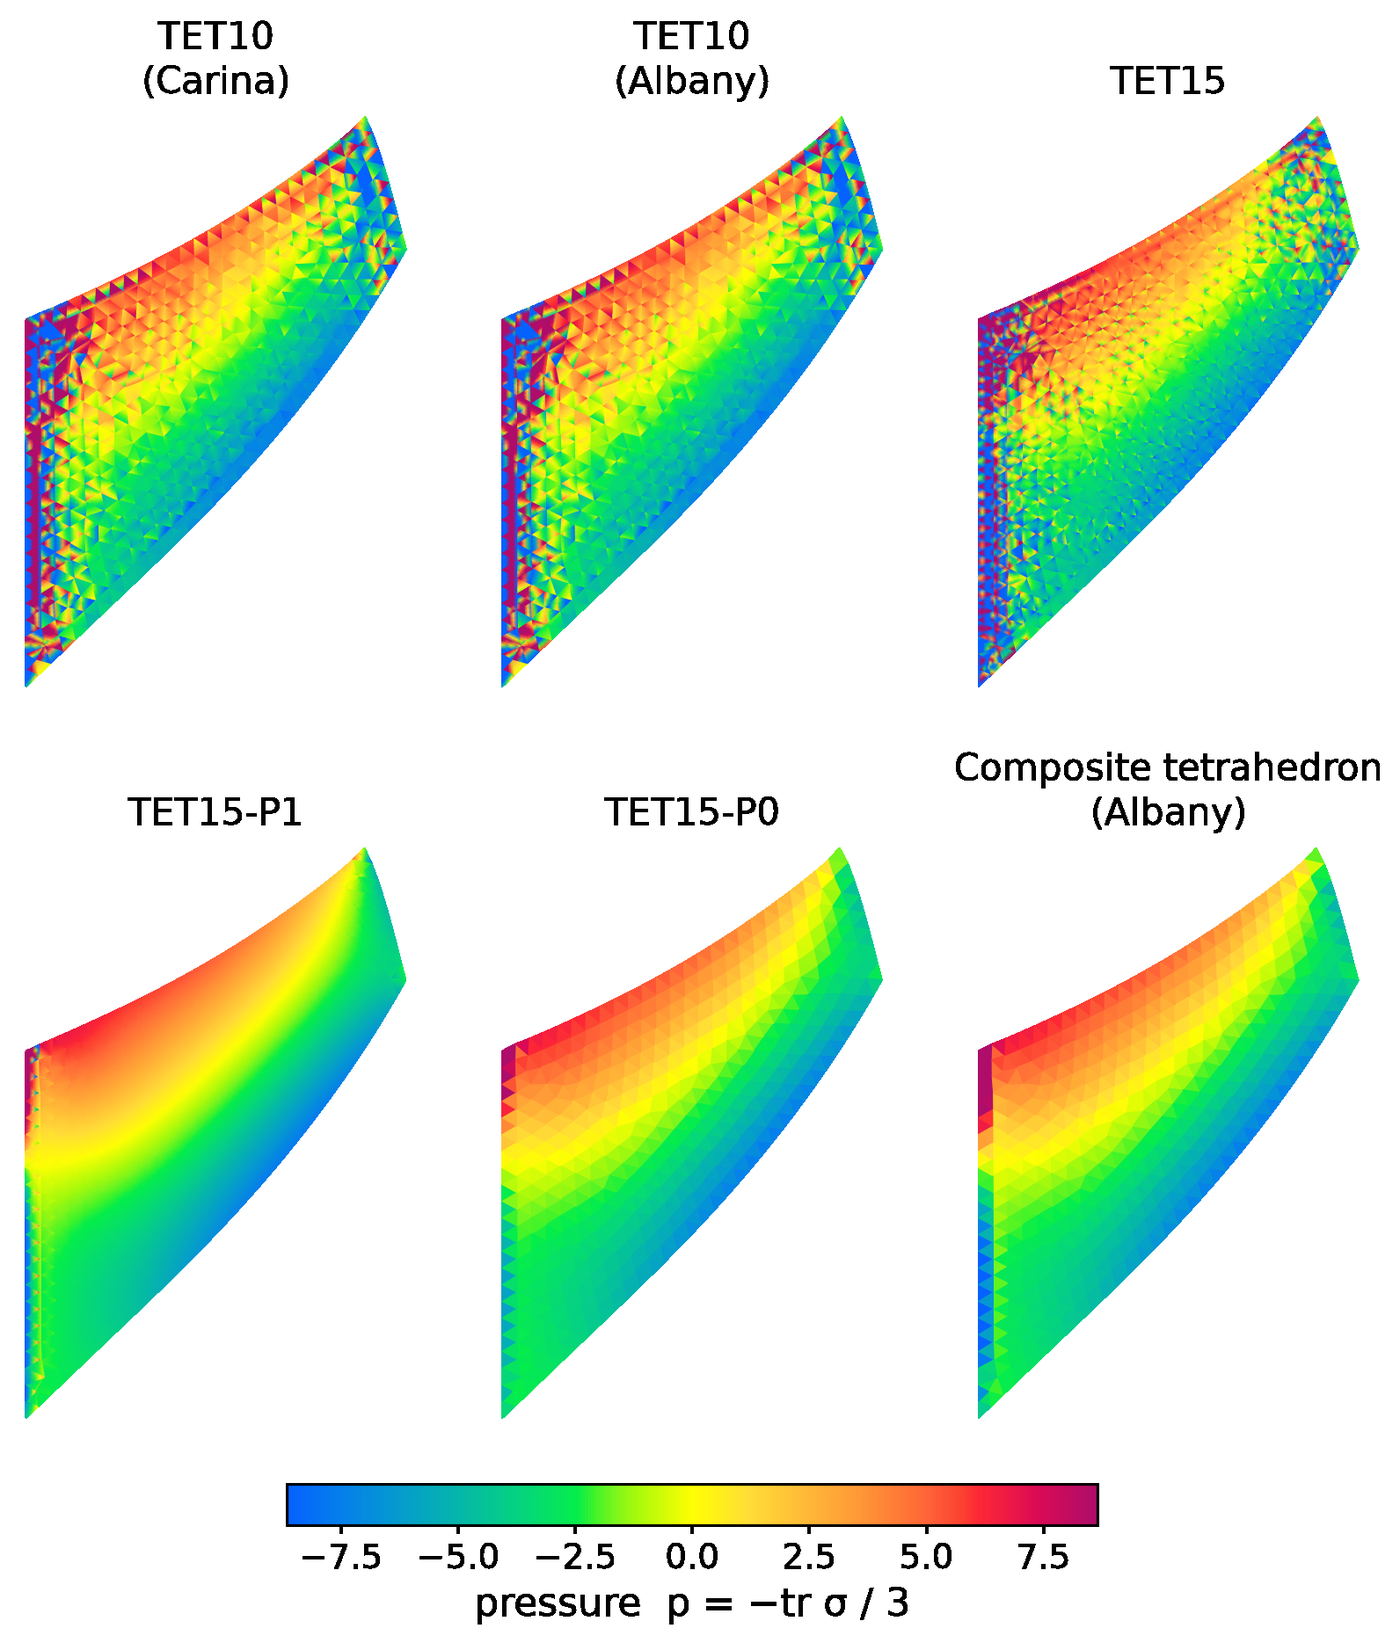
\includegraphics[width=0.92\textwidth]{figures/elastic-h2.png}
\caption{Elastic case, $h = 2$: pressure $p = -\trace~\sigma/3$ on the
face $z = 10$ of the deformed membrane at full load, for the six elements.
One color scale for all panels, symmetric about zero and bounded by the
$99$th percentile of $\lvert p \rvert$ over TET15-P1, TET15-P0
and the composite tetrahedron; values beyond the scale
saturate. Inside each element the pressure drawn is the polynomial fitted to
the quadrature-point values (text).}
\label{fig:elastic-h2}
\end{figure}

\begin{figure}[tbp]
\centering
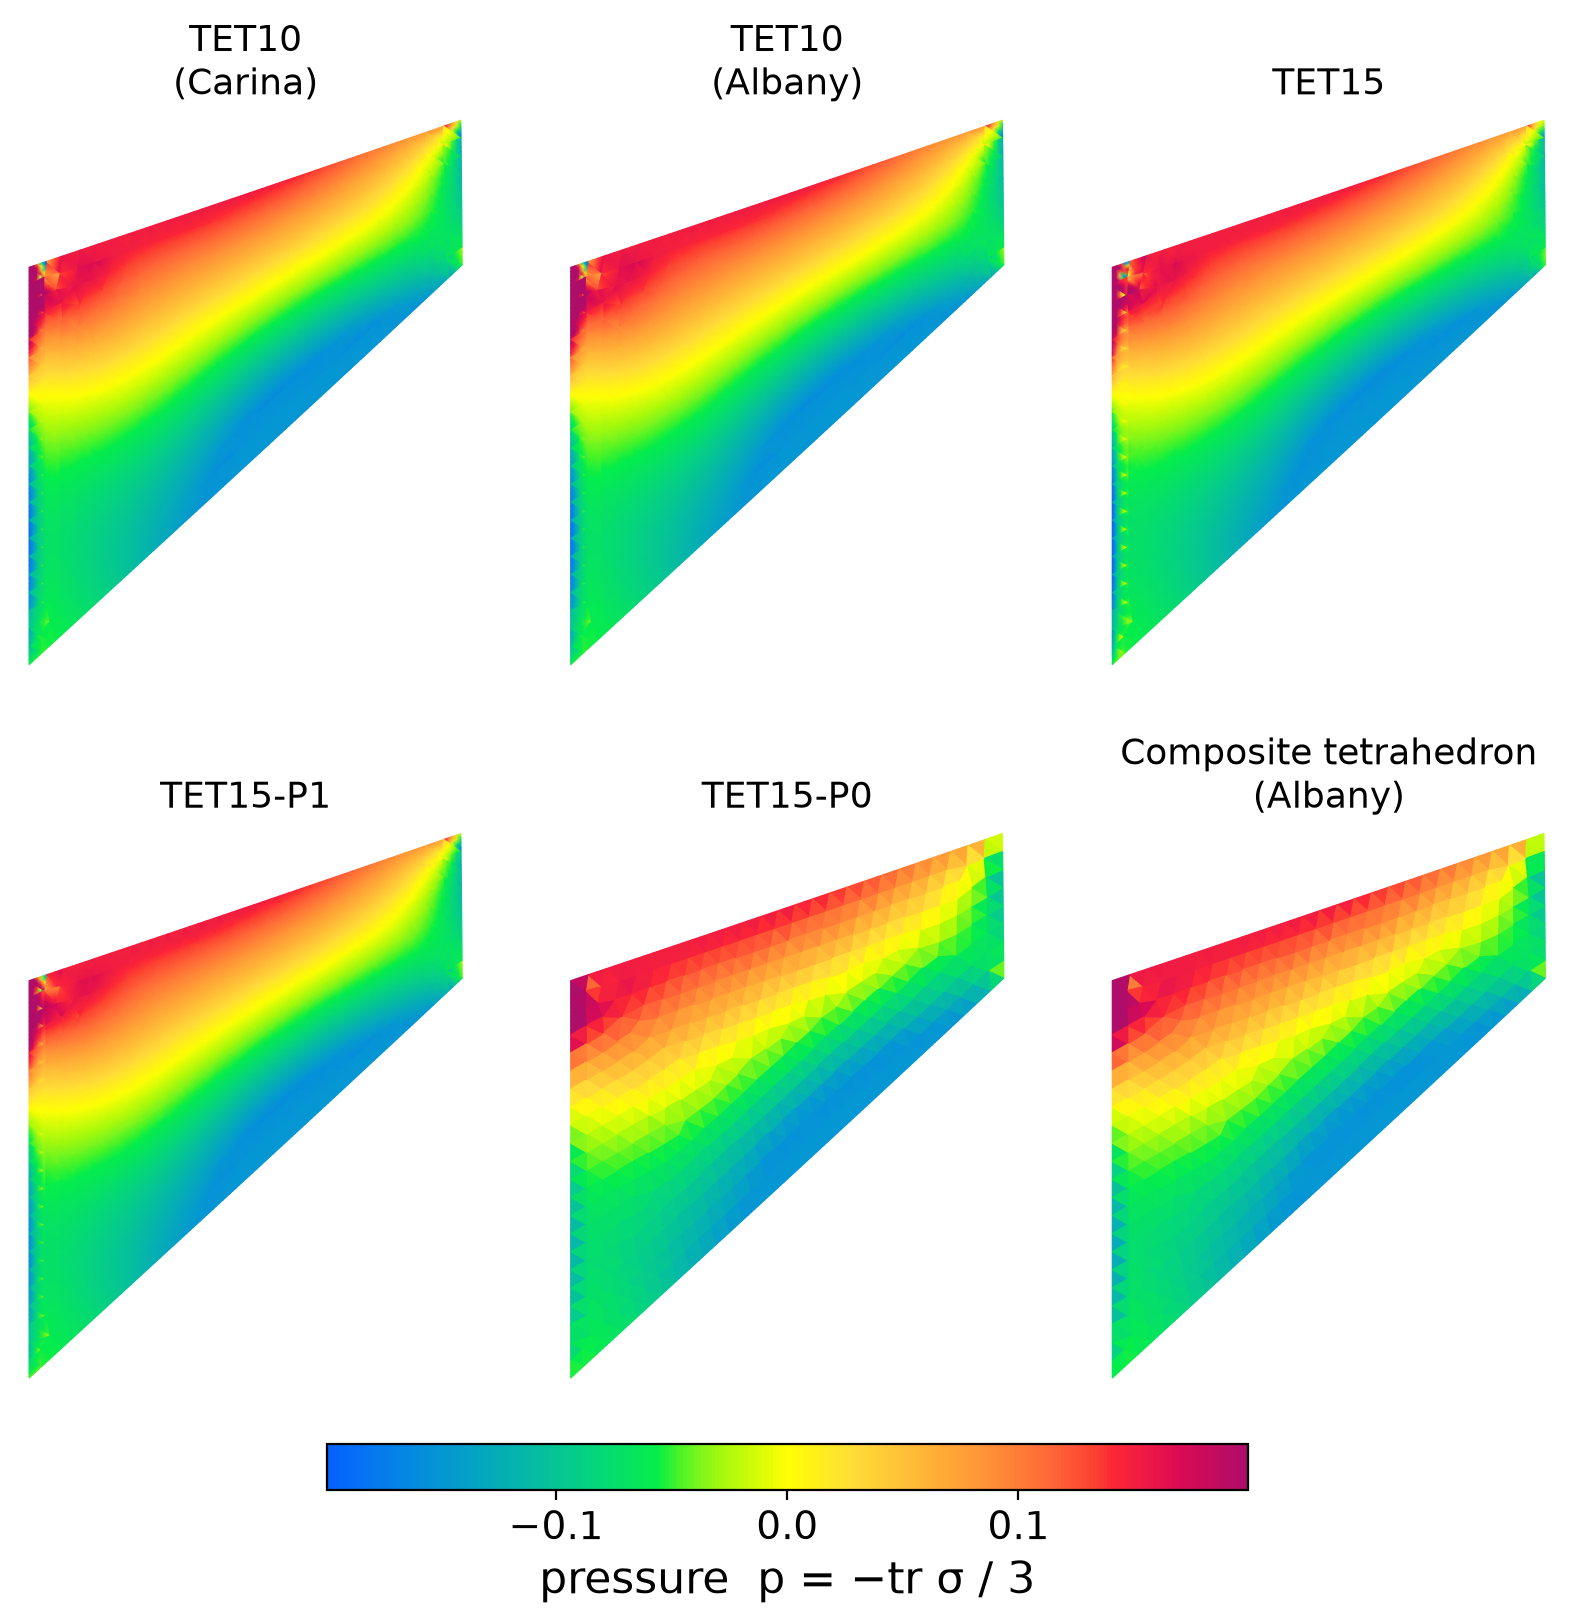
\includegraphics[width=0.92\textwidth]{figures/plastic-h2.png}
\caption{Plastic case, $h = 2$: pressure on the face $z = 10$ at full load,
as in Figure~\ref{fig:elastic-h2}.}
\label{fig:plastic-h2}
\end{figure}

\begin{figure}[tbp]
\centering
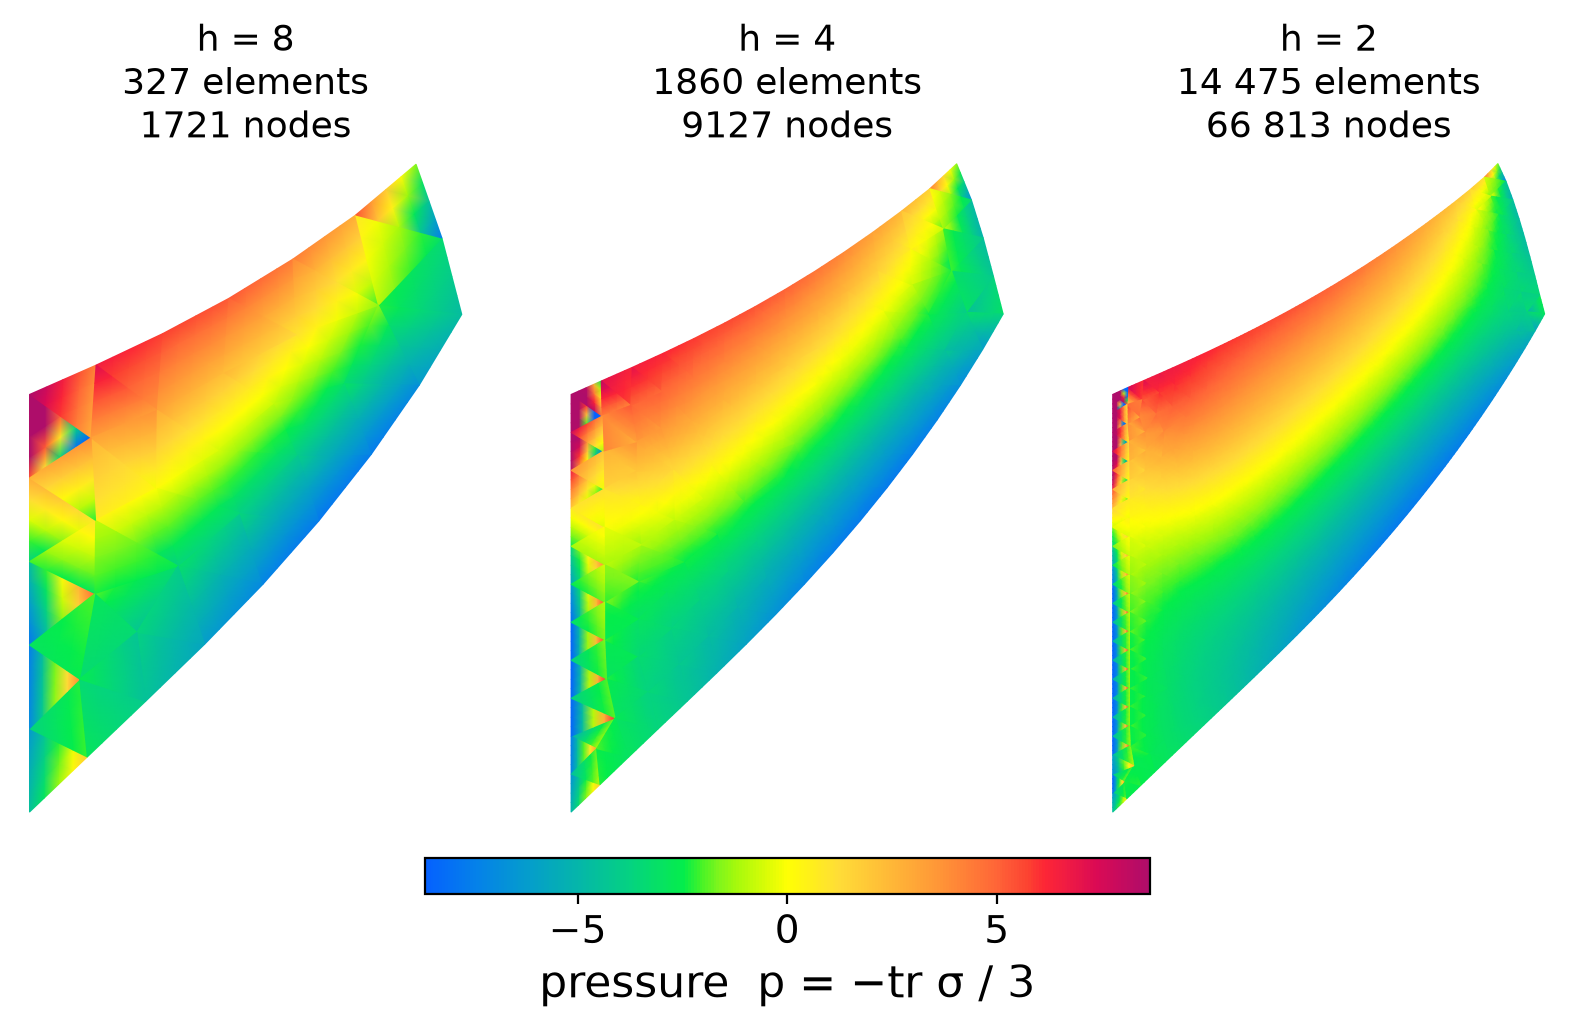
\includegraphics[width=0.48\textwidth]{figures/elastic-tet15-p1-refine.png}\hfill
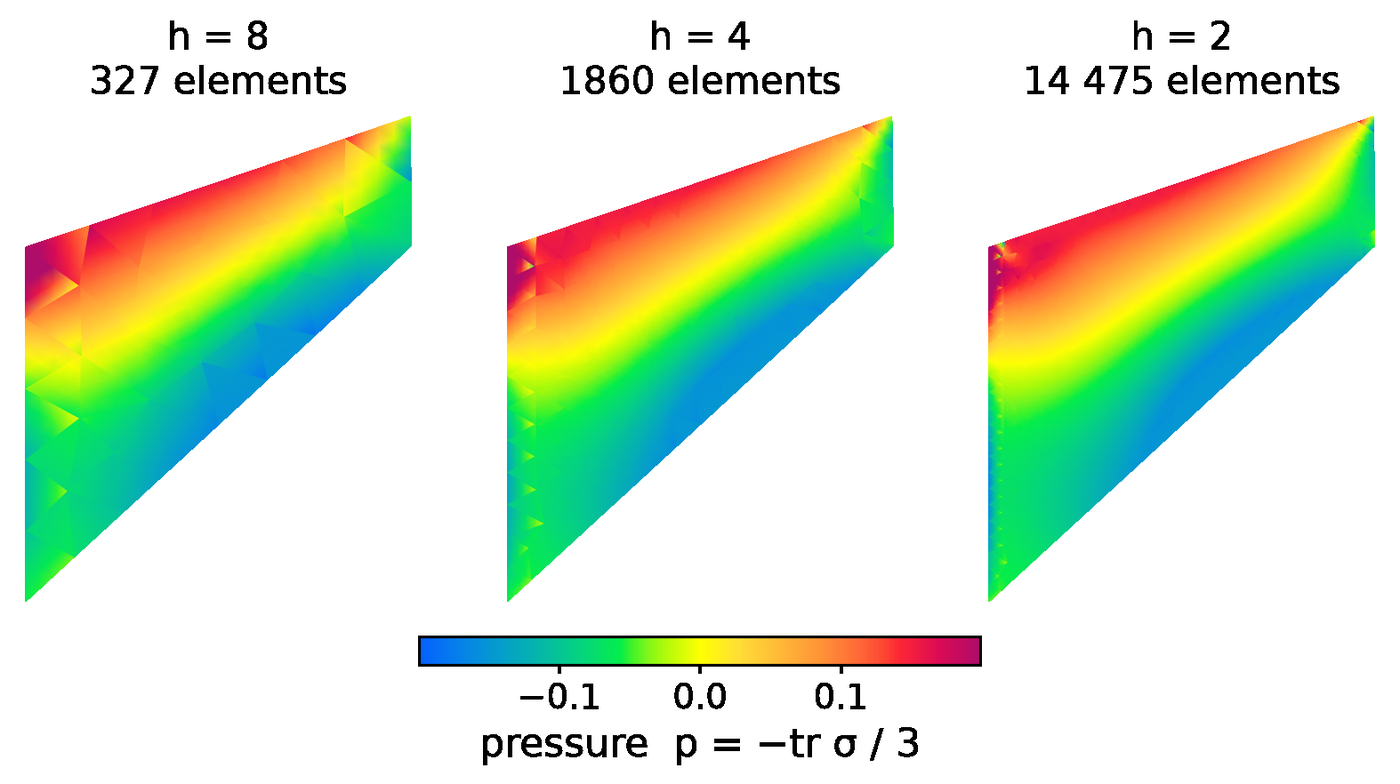
\includegraphics[width=0.48\textwidth]{figures/plastic-tet15-p1-refine.png}\\[0.5em]
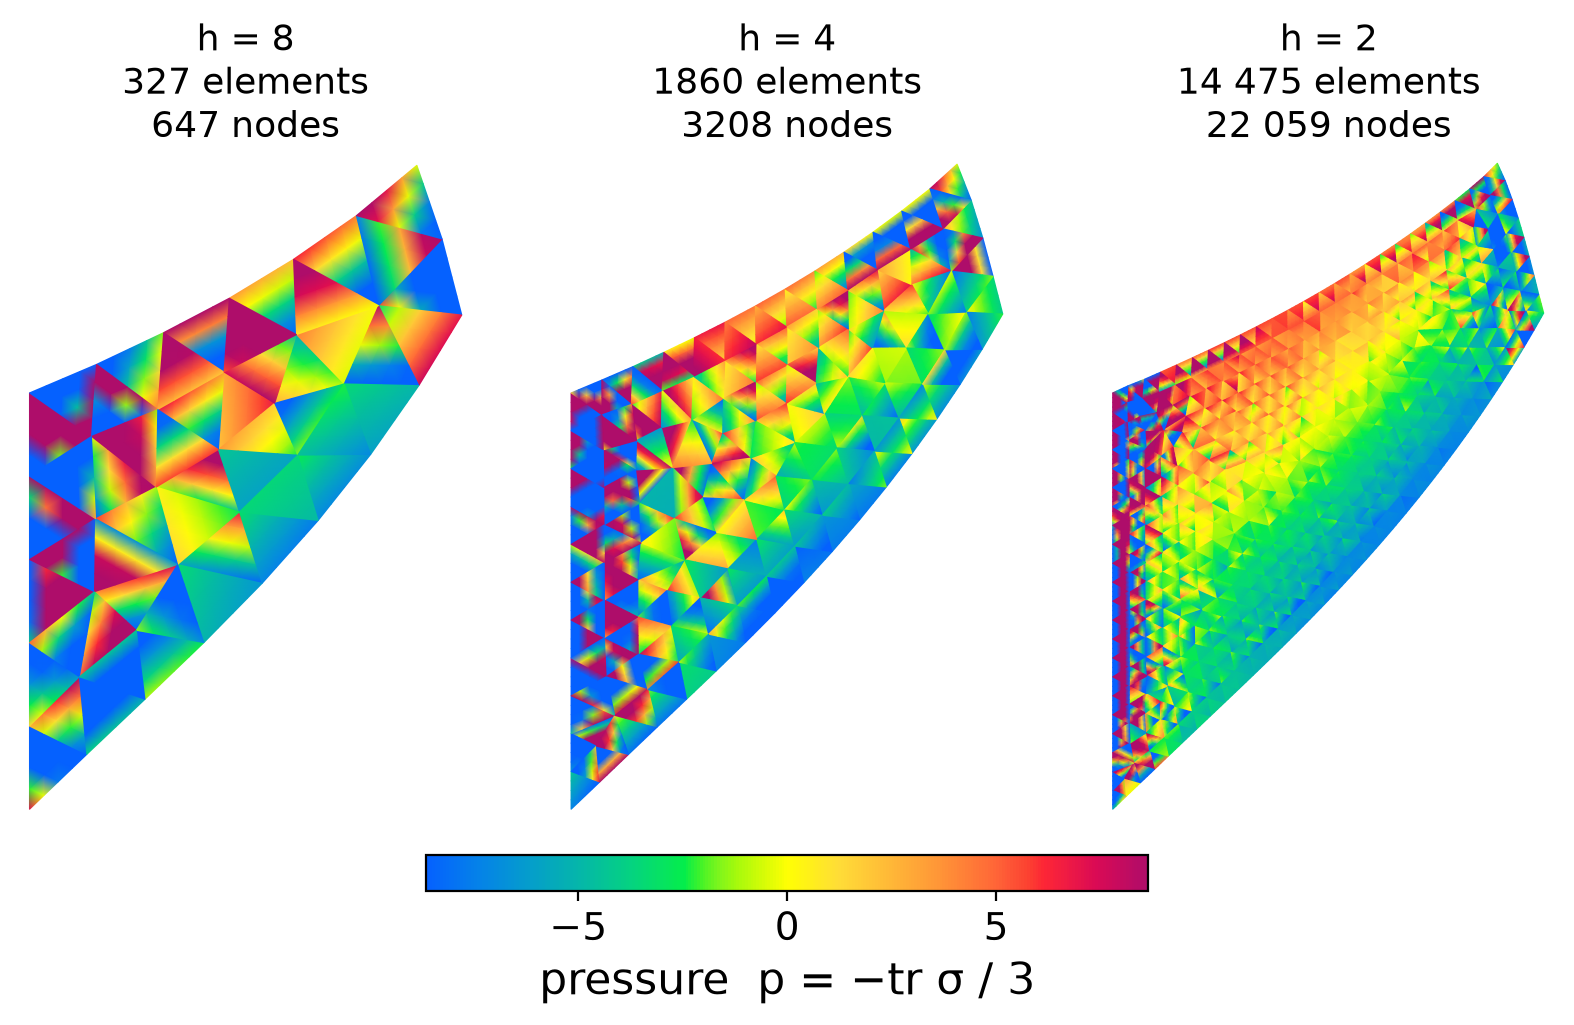
\includegraphics[width=0.48\textwidth]{figures/elastic-tet10-refine.png}\hfill
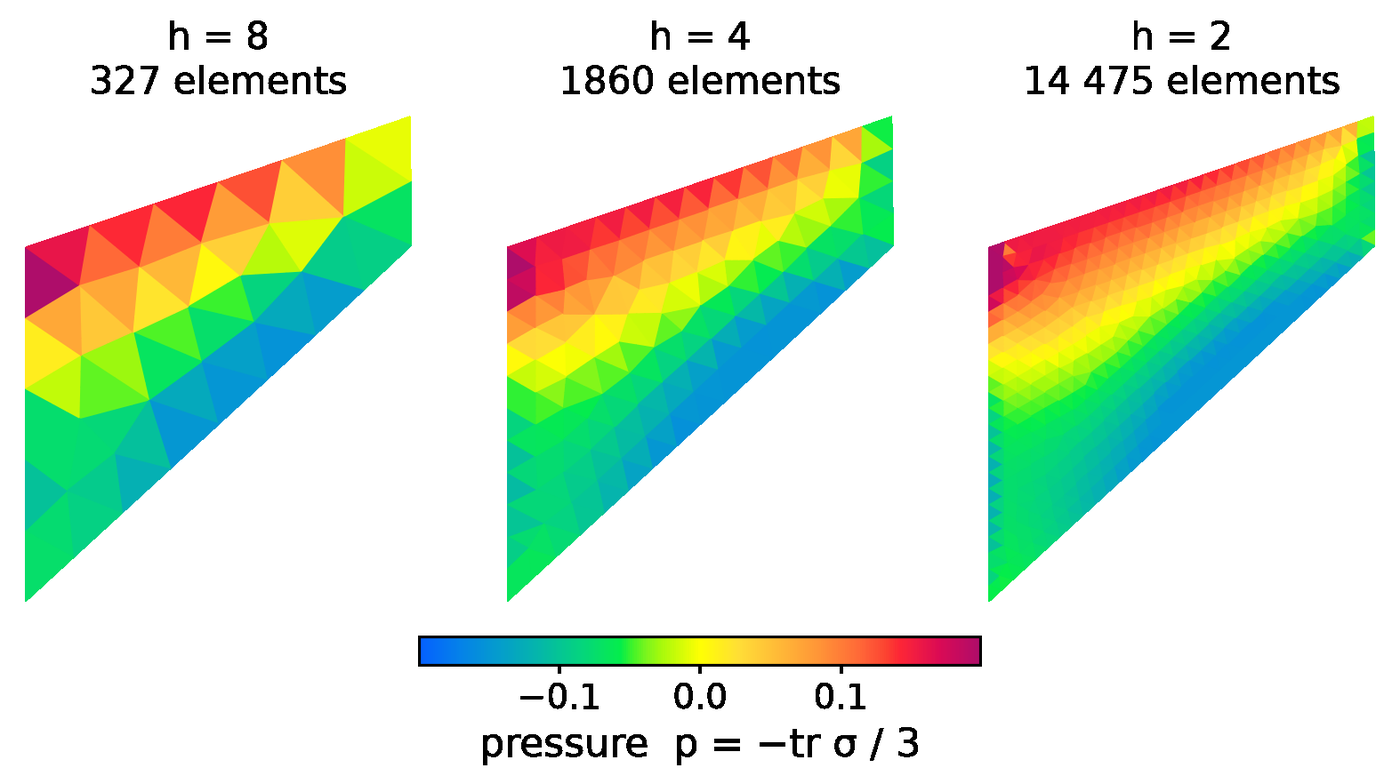
\includegraphics[width=0.48\textwidth]{figures/plastic-lcm-ct-refine.png}
\caption{Pressure on the face $z = 10$ under mesh refinement, $h = 8$, $4$,
$2$ from left to right in each panel, with the color scale of the case.
Top: TET15-P1, elastic (left) and plastic
(right). Bottom left: TET10 pointwise, elastic. Bottom right: the
composite tetrahedron, plastic.}
\label{fig:refine}
\end{figure}

\paragraph{Pressure fields.} The pressure $p = -\trace~\sigma/3$, with
$~\sigma$ the Cauchy stress, is read at the quadrature points of every
element at full load and drawn on the face $z = 10$ of the deformed
membrane (Figures~\ref{fig:elastic-h2}--\ref{fig:refine}). Inside each
element the field drawn is the polynomial fitted to the quadrature-point
values in the least-squares sense with the weights of the rule: quadratic
for the fourteen-point rule of TET15, which reproduces the linear
and the constant projection to rounding error and the pointwise
TET15 pressure, of higher degree, to $0.11$ of its largest value;
linear for the four-point rule of TET10, which interpolates; and
the single value Albany writes per composite tetrahedron. In the elastic
case the pointwise TET10 and TET15 give a pressure that
changes sign inside elements over the whole membrane, on every mesh, with
a range on the face of $-226$ to $211$ and $-512$ to $1010$ at $h = 2$.
TET15-P1 is smooth except in the layer of elements along the
clamped edge, with a range of $-43$ to $61$; TET15-P0 and
the composite tetrahedron are smooth and piecewise constant, with ranges of
$-7.5$ to $22$ and $-9.4$ to $35$. The clamped edge is a singular line of
the continuum solution: where a clamped face meets a free face the stress is
unbounded, and it grows faster as $\nu \to 1/2$. The jumps of TET15-P1
between neighboring elements confirm that the discontinuities
are the element's error at that line and nothing else: at every $h$ the
six largest jumps on the face lie within one element layer of the clamped
edge, the largest $\lvert p \rvert$ of TET15-P1 on the face
grows from $22$ to $35$ to $61$ over the three meshes as an unbounded field
requires, and away from that layer and from the loaded corner the median
jump falls from $3.9\%$ to $0.35\%$ of the color limit from $h = 8$ to
$h = 2$, faster than $h$, whereas for the two piecewise constant elements
it is $12$ to $15\%$ of the color limit at $h = 2$, in proportion to $h$.
In the plastic case no element oscillates, the six fields agree away from
the upper corner of the clamped edge, and the largest pressure on the face
at $h = 2$ is $0.715$ for TET10, $1.15$ for TET15
pointwise, $0.519$ for TET15-P1, $0.292$ for TET15-P0
and $0.407$ for the composite tetrahedron. Scripts:
\code{benchmark/tet15-p1/cook/extract\_pressure.jl} and
\code{render\_pressure.py}.

\paragraph{What the benchmark establishes.} The element of this note does
not lock at $\nu = 0.4999$ on any of the three meshes, agrees in the tip
displacement with the composite tetrahedron within $0.6\%$ and in the limit
of refinement, and gives a pressure that is smooth wherever the continuum
pressure is, on a mesh where the quadratic tetrahedron without projection
gives a pressure that oscillates in sign everywhere. Its unknowns are $3.0$
times those of the composite tetrahedron on the same mesh, the interior
bubble not being condensed in the implementation, and the run times above
are those of one implementation with a direct solver; a comparison at equal
accuracy is not made. The equivalent plastic strain is
not measured here: at $q = 0.14$ the plastic zone of the membrane does not
lock any of the quadratic elements, so the membrane does not separate them
on that quantity.

\section{Explicit dynamics: the Taylor bar impact}
\label{sec:taylor}

This section measures the element in explicit dynamics with plastic
strains above $3$, against the composite tetrahedron of Sierra/SM, the code
of \citet{Foulk.etal:2021}, on the same meshes. The quantity measured is
the final radius of the impact face, for which a converged reference value
exists; the equivalent plastic strain is not measured.

\paragraph{Problem.} A copper bar of length $32.4$~mm and radius $3.2$~mm,
with its axis along $z$, strikes a rigid frictionless wall at $z = 0$ with
velocity $227$~m/s \citep{WilkinsGuinan:1973,Simo:1992,Foulk.etal:2021}.
The material has density $\rho = 8930$~kg/m$^3$, Young's modulus
$E = 117$~GPa, Poisson's ratio $\nu = 0.35$ ($\kappa/\mu = 3.0$; the
plastic flow is isochoric, so the response in the plastic zone is nearly
incompressible), yield
stress $400$~MPa and a linear isotropic hardening modulus of $100$~MPa; the
Simo--Hughes $J_2$ model (Remark~\ref{rem:whichj2}) in Carina and the
finite-deformation $J_2$ model of the Sierra material library, with the
same constants. The wall is the condition $u_z = 0$ on the impact face,
which is in contact at $t = 0$ and remains in contact while the bar moves
toward the wall. The equations are integrated by central differences with
the row-sum lumped mass of \S\ref{sec:dynamics} to $t = 80~\mu$s, without
artificial bulk viscosity. The measured quantities are the radius of the
impact face, the largest distance of its nodes from the axis, and the
length of the bar, the largest $z$ of its free end, at every microsecond.
\citet{Foulk.etal:2021} give $7.22$~mm for the final radius of the
eight-node hexahedron with constant pressure (Q1/P0) on their finest mesh,
$h = 0.047$~mm, which is the reference here; \citet{Simo:1992} gives
$7.12$~mm and \citet{ZienkiewiczEtAl:1998} $7.11$~mm on coarser meshes.

\paragraph{Meshes and elements.} Four levels, $h = 1.5$, $0.75$, $0.38$ and
$0.19$~mm, of the full bar are meshed by Cubit with four-node tetrahedra,
the Cubit size being adjusted until the element count is within $3\%$ of
that of \citet[Figure~14]{Foulk.etal:2021}: $3522$, $25\,029$,
$190\,727$ and $1\,521\,212$ elements, with $5601$, $36\,666$, $267\,150$
and $2\,083\,320$ nodes as \code{TETRA10} meshes and $16\,587$, $113\,331$,
$845\,573$ and $6\,672\,877$ as \code{TETRA15} meshes. Each mesh is smoothed by the
energetic mesh smoothing of Norma, which minimizes a strain energy of the
mesh over the positions of its nodes with every boundary node held on its
surface; this raises the smallest shape quality
$q = 12\,(3V)^{2/3} / \sum_{e} l_e^2$, with $V$ the volume and $l_e$ the
six edge lengths, from $0.58$--$0.65$ to $0.69$--$0.71$ at every level. The
edge midpoints are added with those on the lateral surface projected onto
the cylinder (\code{TETRA10}, the mesh of the composite tetrahedron), and
the face and interior nodes are added by the conversion of
\S\ref{sec:element} (\code{TETRA15}). Three elements are compared:
TET15-P1 and TET15-P0 in Carina, and the composite tetrahedron in Sierra/SM
with its stabilization parameter $\alpha = 0.1$ and the stabilization
exponent $0$ of \citet{Foulk.etal:2021}. The displacement unknowns of
TET15 are $49\,761$, $339\,993$ and $2\,536\,719$ on the first three
levels; those of the composite tetrahedron are $109\,998$, $801\,450$ and
$6\,249\,960$ on the second to fourth.

\paragraph{Stable time step.} The step of central differences is stable
when $\Delta t \le 2/\sqrt{\lambda_{\max}}$, with $\lambda_{\max}$ the
largest eigenvalue of $M_L^{-1} K$, $M_L$ the lumped mass and $K$ the
tangent stiffness. The runs of Table~\ref{tab:taylor} set the step to a
Courant number of $0.25$ times an element estimate, the smallest distance
between two nodes of an element divided by the dilatational wave speed
$c_p$, recomputed every ten steps on the current configuration. That
estimate is not a bound: $\lambda_{\max}$ computed by power iteration on
the TET15-P1 run at $h = 0.75$~mm gives a ratio of the critical step to the
element estimate of $1.14$ at $1~\mu$s, $1.02$ at $10~\mu$s, $0.69$ at
$20~\mu$s, $0.42$ at $28~\mu$s, $0.31$ at $40~\mu$s and $0.29$ at $60$ and
$80~\mu$s. At a Courant number of $0.5$ the run stopped with a non-finite
residual at $28~\mu$s; at $0.25$ it reached $80~\mu$s with a step $0.82$
times the critical one at $40~\mu$s; TET15-P0 at $h = 0.38$~mm stopped at
$78.7~\mu$s, and its radius at $78~\mu$s is reported, the radius being
constant within $0.06\%$ after $50~\mu$s for every element
(Figure~\ref{fig:taylor}). Carina
also offers the step $0.8 \cdot 2/\sqrt{\lambda_{\max}}$, with
$\lambda_{\max}$ computed every $200$ steps and the element estimate scaled
by the ratio of the two in between; on the same run it takes $43\,863$
steps against about $54\,000$ at the Courant number $0.25$, and the final
radius differs by $0.0007$~mm.

\begin{table}[tbp]
\centering
\caption{Taylor bar, final radius of the impact face and final length of
the bar in mm at $80~\mu$s, per element and mesh level $h$ in mm with its
element count. Reference: $7.22$ for the converged Q1/P0 hexahedron
\citep{Foulk.etal:2021}. TET15-P0 at $h = 0.38$ stopped at $78.7~\mu$s;
its values at $78~\mu$s. The composite tetrahedron at $h = 1.5$ ended at
$41.6~\mu$s. Driver: \code{benchmark/tet15-p1/taylor/run.jl}; histories in
\code{benchmark/tet15-p1/taylor/data}.}
\label{tab:taylor}
\begin{tabular}{rr cc cc cc}
\toprule
 & & \multicolumn{2}{c}{TET15-P1} & \multicolumn{2}{c}{TET15-P0}
 & \multicolumn{2}{c}{composite tet.} \\
$h$ & elements & radius & length & radius & length & radius & length \\
\midrule
$1.5$  & $3522$          & $7.2399$ & $21.4250$ & $7.4415$ & $21.5507$ & --- & --- \\
$0.75$ & $25\,029$       & $7.2225$ & $21.4206$ & $7.4747$ & $21.5329$ & $7.2820$ & $21.4760$ \\
$0.38$ & $190\,727$      & $7.2255$ & $21.4202$ & $7.3785$ & $21.4763$ & $7.2453$ & $21.4395$ \\
$0.19$ & $1\,521\,212$   & --- & --- & --- & --- & $7.2326$ & $21.4304$ \\
\bottomrule
\end{tabular}
\end{table}

\begin{figure}[tbp]
\centering
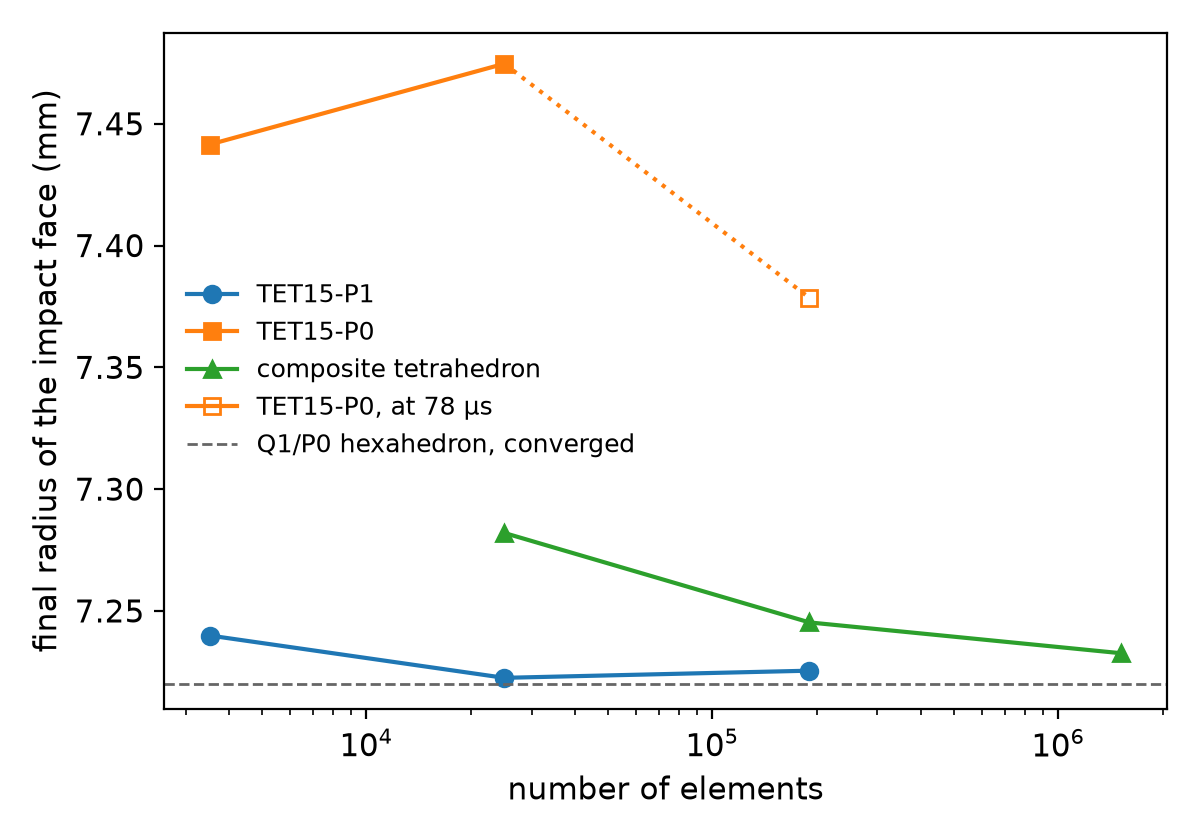
\includegraphics[width=0.49\textwidth]{figures/taylor-convergence.png}\hfill
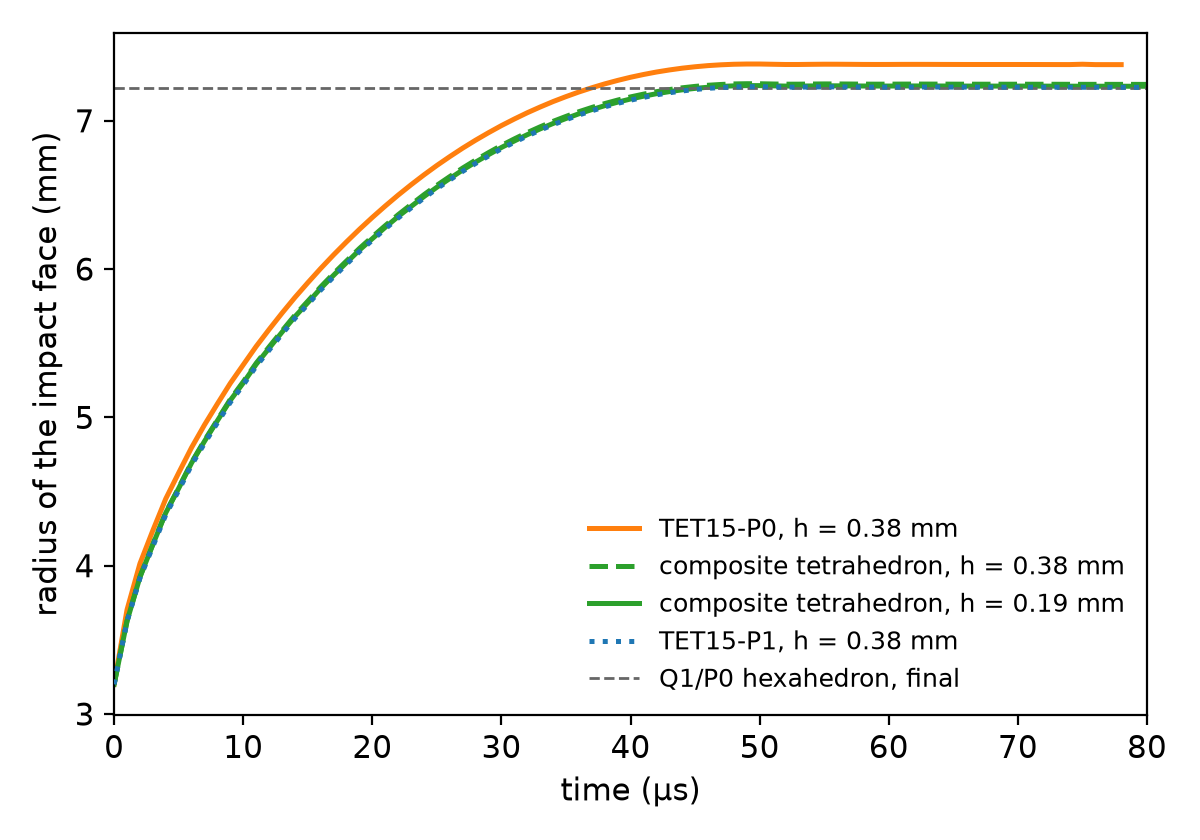
\includegraphics[width=0.49\textwidth]{figures/taylor-history.png}
\caption{Taylor bar. Left: final radius of the impact face against the
number of elements; the open square is TET15-P0 at $78~\mu$s. Right: radius
of the impact face against time for TET15-P1 and TET15-P0 at
$h = 0.38$~mm and the composite tetrahedron at $h = 0.38$ and $0.19$~mm.
Dashed gray: the converged Q1/P0 hexahedron of \citet{Foulk.etal:2021}.
Script: \code{benchmark/tet15-p1/taylor/plot.py}.}
\label{fig:taylor}
\end{figure}

\paragraph{Accuracy.} Table~\ref{tab:taylor} and Figure~\ref{fig:taylor}.
The composite tetrahedron converges from above: its differences between
successive levels are $0.0367$ and $0.0127$~mm, a ratio of $2.89$, which
corresponds to an order of $1.53$ in $h$; the extrapolation of its three
levels by that ratio gives $7.2259$~mm. TET15-P1 is at $7.2225$ and
$7.2255$~mm at $h = 0.75$ and $0.38$, within $0.05\%$ of that value, and
at $7.2399$ on the coarsest mesh, where the composite tetrahedron did not
reach $80~\mu$s. The composite tetrahedron is $0.78\%$, $0.27\%$ and
$0.09\%$ from the extrapolated value at $h = 0.75$, $0.38$ and $0.19$. Both
elements approach the reference within $0.1\%$ in the limit. TET15-P0 is
$3.4\%$ above the extrapolated value at $h = 0.75$ and $2.1\%$ at
$h = 0.38$; it differs from TET15-P1 only in the constant pressure.

\paragraph{Operations.} The two codes were run on the same machine, a
two-socket AMD EPYC 9634 with $168$ cores, one run at a time with no other
job, at $h = 0.75$~mm (Table~\ref{tab:taylorcost}). Per element and time
step on one core, TET15-P1 takes $1.40$ times the time of the composite
tetrahedron; per element degree of freedom, $45$ against $30$, it takes
$0.93$ times as long. On $16$ cores the ratio per element and step is
$3.0$, because Carina's time per step decreases by a factor of $6.5$ from
$1$ to $16$ threads, a parallel efficiency of $0.40$, against $0.88$ for
Sierra/SM on $16$ processes; the difference is in the implementation of the
time step in Carina, not in the element. The time step of TET15-P1 at $t = 0$ is
$3.86 \times 10^{-9}$~s under the element estimate at the Courant number
$0.25$, and its critical step is $1.77 \times 10^{-8}$~s; that of the
composite tetrahedron is $2.44 \times 10^{-8}$~s.

\begin{table}[tbp]
\centering
\caption{Taylor bar at $h = 0.75$~mm ($25\,029$ elements), both codes on
the same two-socket AMD EPYC 9634, each run alone. One-core figures from
runs to $5~\mu$s. Core-$\mu$s: wall time times the number of cores.
Memory of Sierra/SM: the largest of its processes.}
\label{tab:taylorcost}
\small
\begin{tabular}{lcc}
\toprule
 & TET15-P1 (Carina) & composite tet.\ (Sierra/SM) \\
\midrule
per element and step, 1 core ($\mu$s)          & $6.27$ & $4.47$ \\
per element and step, 16 cores (core-$\mu$s)   & $15.5$ & $5.09$ \\
steps to $80~\mu$s                              & $52\,100$ & $44\,260$ \\
time stepping to $80~\mu$s on 16 cores (s)     & $1265$ & $352$ \\
largest resident memory (GB)                    & $1.63$ & $0.27$ \\
final radius (mm)                               & $7.2225$ & $7.2820$ \\
\bottomrule
\end{tabular}
\end{table}

\paragraph{Comparison at equal accuracy.} TET15-P1 at $h = 0.75$~mm is
closer to the extrapolated radius ($0.05\%$) than the composite
tetrahedron at $h = 0.19$~mm ($0.09\%$). On the machine above, each run
alone, the first takes $1303$~s on $16$ cores, $2.1 \times 10^{4}$
core-seconds, and the second $10\,983$~s on $128$ processes,
$1.41 \times 10^{6}$ core-seconds: a factor of $67$ in core-seconds and of
$8.4$ in wall time, on $25\,029$ elements against $1\,521\,212$. At equal
mesh the composite tetrahedron takes $3.6$ times less time to $80~\mu$s on
$16$ cores, with an error $16$ times larger.

\paragraph{The same run on GPUs.} The explicit integration of TET15-P1
runs on a GPU through the same kernels, with the stable step recomputed on
the device. At $h = 0.75$~mm with the global stable step, the radius and the
length of every output frame of the run are the same numbers to every
written digit on the CPU, on an AMD RX~7600 and on NVIDIA L4, V100, A100
and H100 cards (the last four on one mesh, the first two on another smoothing
of the same Cubit mesh, which changes the radius by $2.8\times10^{-7}$
relative),
and so are the $221$ stable-step estimates. Table~\ref{tab:taylordevices}
gives the time per step from the kernel timings and the wall time of the
run. Three defects were found and corrected in making these runs: the
stable-step recomputation read the block sizes and the material properties
through accessors defined for host arrays only, so it had never run on a
device; the temporaries of the explicit step (about $0.65$~MB per step at
$340\,000$ unknowns) are released only when the garbage collector runs,
which host pressure did not trigger, so the run exhausted the $8$~GB of the
RX~7600 after about $5\,000$ steps, and the collector is now run every
$100$ steps on a device; and the $J_2$ tangent of the material library
built its pull-back in mutable buffers that CUDA places on the device heap,
which is never freed, so the matrix-free solves of the implicit tests failed
on the L4 after some thousands of tangent calls (the buffers are now
immutable, and the tangent is $5\%$ faster on every device). The eigenvalue
estimate of the stable step runs $20$ to $40$ power iterations, each two
residual evaluations, every $200$ steps. Its share of the run, from the
saving of the adaptive interval below, is $14.8\%$ on the RX~7600, $14.4\%$
on the L4, $11.4\%$ on the V100 and about $3\%$ on the H100. An earlier
estimate of $25$ to $40\%$ on the GPUs, from a single timed estimate, was
too high: timed once right after the warm-up of the timing script, the
estimate took $1.5$ to $4.4$ times the median of five. A fixed longer interval is not
safe: the ratio of the eigenvalue step to the element estimate falls by up
to $11\%$ between two estimates $200$ steps apart while the bar spreads,
between $8$ and $30~\mu$s, and by up to $23\%$ within $1000$ steps, more
than the $20\%$ margin of CFL $0.8$; after $30~\mu$s it varies by at most
$1.3\%$ per $200$ steps, and after $60~\mu$s by $0.04\%$. Carina therefore
sets the interval from the observed change (input key \code{stable time step
eigenvalue change}~$c$): after each estimate the next interval is the one
over which the relative decrease of the ratio observed over the last
interval would amount to $c$, at least the given interval, at most twice the
last one and at most $16$ times the given one. With $c = 0.02$ the run at
$h = 0.75$~mm on the RX~7600 takes $52$ estimates instead of $220$, at
intervals from $200$ to $3200$ steps, $43\,557$ steps instead of
$43\,865$, and $443$ instead of $500$~s, with the radius and length
histories equal to within $7\times10^{-7}$ relative; the same runs take
$399$ instead of $449$~s on the L4, $367$ instead of $402$~s on the V100 and
$155$ instead of $159$~s on the H100 (a difference within the variation
between runs), with the same histories, frame for frame, on the four NVIDIA
cards. Applied to the ratios
recorded with the fixed interval, the rule keeps the largest decrease of the
ratio within an interval at the one over $200$ steps.

\begin{table}[tbp]
\centering
\caption{TET15-P1, split form, explicit Taylor bar: time per step of a run
from the kernel timings (median of $20$, deformed state with plastic strains
to $1.0$; includes the stable-step estimates at their intervals), in
microseconds per element-step, at $h = 0.75$ and $0.38$~mm, the ratio of the
general form's time to the split form's at $h = 0.75$~mm, and the wall time
of the run to $80~\mu$s at $h = 0.75$~mm. GPU rows and the Ryzen row:
Carina 36b4a9f and 178e811, the eigenvalue estimate as the median of five
(2026-10-06). EPYC rows ($^{*}$): Carina 9e4bfaf, the eigenvalue estimate
timed once (2026-10-04), which on a CPU agrees with the median (on the Ryzen
$459.6$ against $457.1$~ms). Wall times: Carina 9e4bfaf, the H100 36b4a9f.
One process alone on each GPU. Scripts:
\code{benchmark/tet15-p1/taylor/kernel\_timing.jl}, \code{timing\_table.py};
records in \code{data/}.}
\label{tab:taylordevices}
\small
\begin{tabular}{lrrrr}
\toprule
device & $h = 0.75$ & $h = 0.38$ & general/split & run (s) \\
\midrule
AMD Ryzen~9 9900X, 12 threads  & 0.704 & ---   & 1.39 & 839 \\
2$\times$AMD EPYC 9634, 32 threads$^{*}$ & 0.700 & 0.772 & 1.36$^{\dagger}$ & 1283$^{\dagger}$ \\
2$\times$AMD EPYC 9634, 64 threads$^{*}$ & 0.836 & 0.652 & --- & --- \\
AMD RX 7600                    & 0.430 & ---   & 1.42 & 513 \\
NVIDIA L4                      & 0.321 & 0.279 & 1.71 & 406 \\
NVIDIA V100                    & 0.271 & 0.209 & 2.27 & 404 \\
NVIDIA A100                    & 0.119 & 0.097 & 2.18 & 227 \\
NVIDIA H100                    & 0.069 & 0.052 & 2.43 & 159 \\
\bottomrule
\end{tabular}

\smallskip
$^{\dagger}$at 16 threads.
\end{table}

\paragraph{Pressure field.} Figure~\ref{fig:taylorpressure} shows the
pressure $p = -\tfrac13\trace ~\sigma$, positive in compression, on the impact
face at $t = 12~\mu$s, the time of Figure~12 of \citet{Foulk.etal:2021},
for both elements on the same meshes. The composite tetrahedron has one
value per element, the element mean of the stress that Sierra/SM writes;
for TET15-P1 the pressure in each element is the quadratic fitted to its
fourteen quadrature-point values, as in \S\ref{sec:cook}. The largest
pressure on the impact end is $0.33$, $0.48$, $1.37$ and $1.59$~GPa for the
composite tetrahedron at $h = 1.5$, $0.75$, $0.38$ and $0.19$~mm, and
$1.67$, $1.58$, $1.56$ and $1.54$~GPa for TET15-P1, between $3\%$ below
and $5.2\%$ above the composite tetrahedron's value on its finest mesh at
every level; on that mesh the two differ by $3\%$. On the two coarser meshes the pressure of the composite tetrahedron
varies from element to element without a maximum on the axis; TET15-P1
gives the maximum on the axis on every mesh. The radius of the impact face
at $12~\mu$s is $5.4944$, $5.4957$, $5.4750$ and $5.4661$~mm for the
composite tetrahedron and $5.4517$, $5.4507$, $5.4533$ and $5.4570$~mm for
TET15-P1.
\citet{Foulk.etal:2021} plot the $L^2$ projection of the composite
tetrahedron's pressure onto a continuous field, and the range of their color
scale, $-1.2$ to $0.32$~GPa, indicates the mean stress $\tfrac13\trace ~\sigma
= -p$. Scripts: \code{benchmark/tet15-p1/taylor/pressure.jl},
\code{render\_pressure.py} and \code{compose\_pressure.py}.

\begin{figure}[tbp]
\centering
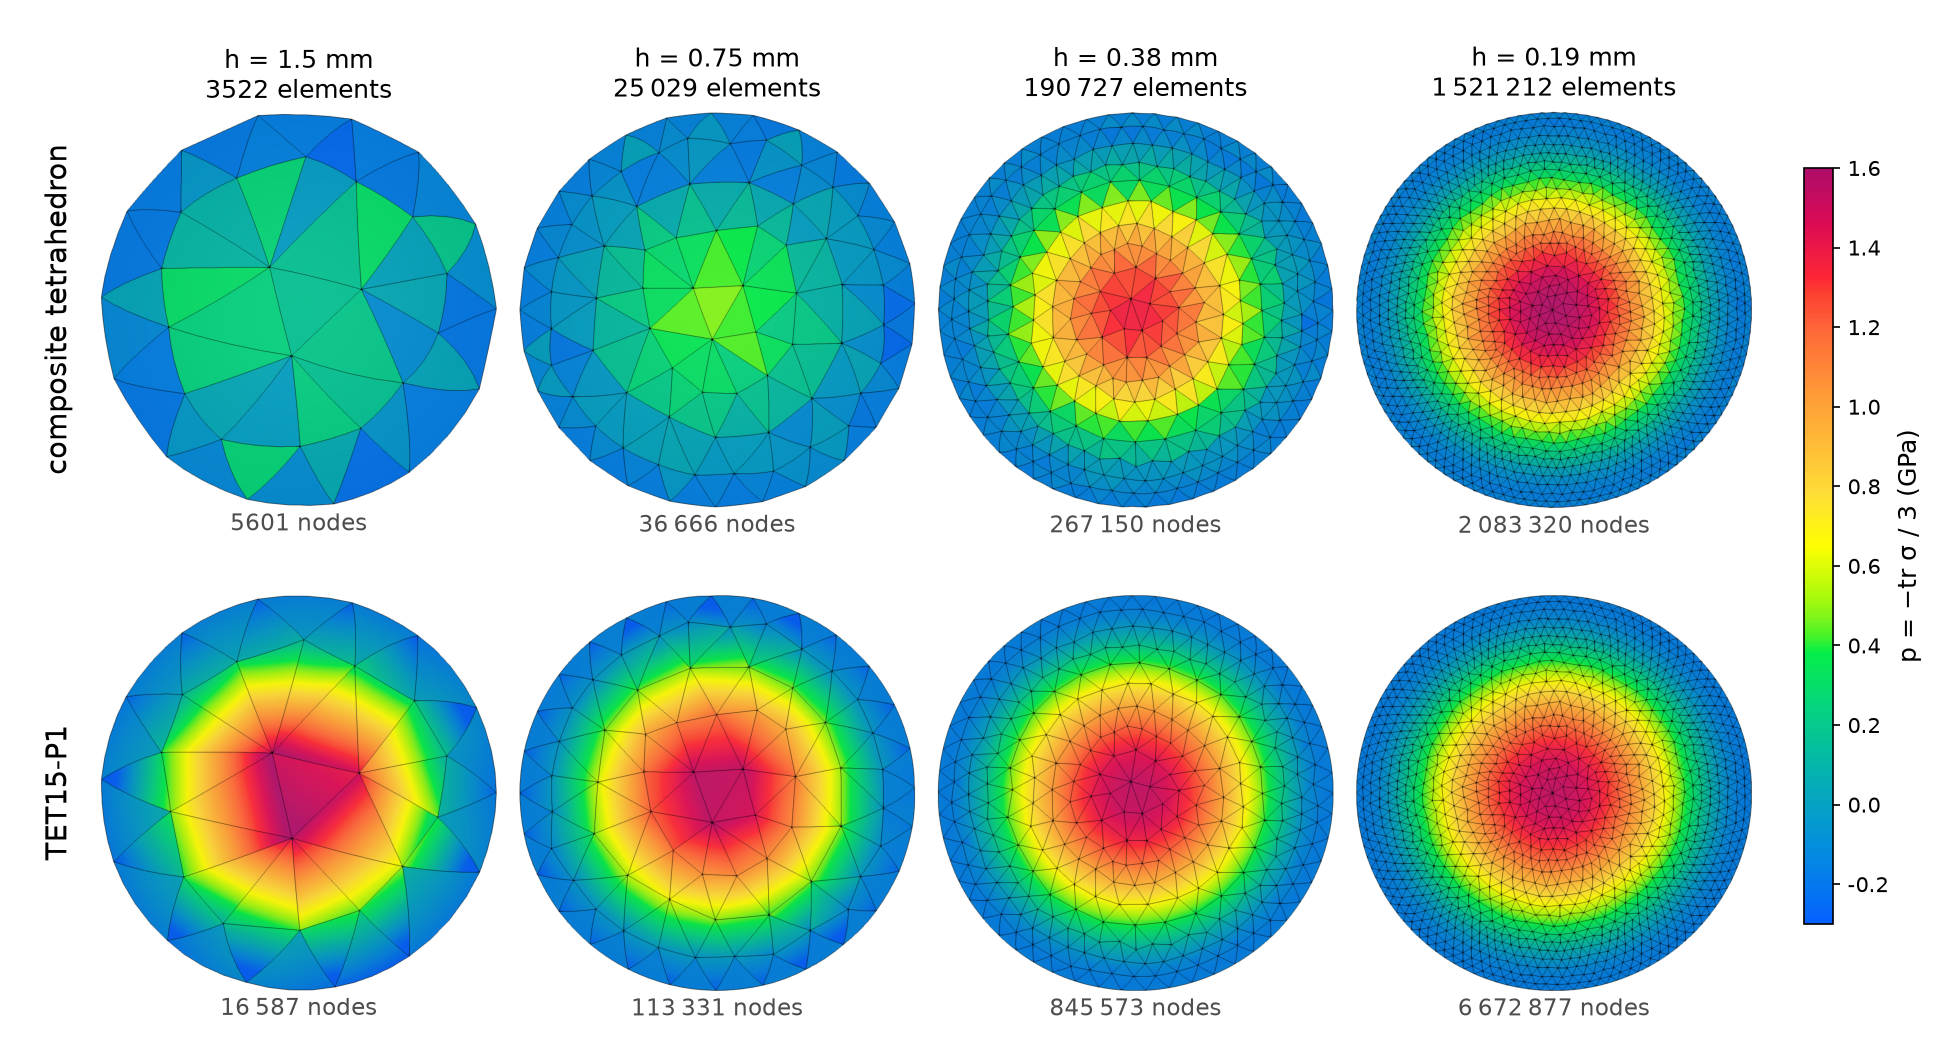
\includegraphics[width=\textwidth]{figures/taylor-pressure-face.png}
\caption{Taylor bar, pressure $p = -\tfrac13\trace ~\sigma$ on the impact face
at $t = 12~\mu$s, seen along the axis, on the same meshes for both
elements, with the element count of each level and the node count of each
mesh (\code{TETRA10} for the composite tetrahedron, \code{TETRA15} for
TET15-P1); one color scale, values beyond it saturate. Top: composite
tetrahedron (Sierra/SM, $\alpha = 0.1$, exponent $0$), one value per
element. Bottom: TET15-P1, the quadratic fitted in each element.}
\label{fig:taylorpressure}
\end{figure}

\paragraph{What the benchmark establishes.} In explicit dynamics with plastic
strains above $3$, TET15-P1 gives the final radius of the Taylor bar within
$0.05\%$ of the converged value on a mesh of $25\,029$ elements, where the
composite tetrahedron needs $1.5$ million elements to reach $0.09\%$, and
the constant-pressure variant on the same displacement space is $2.1$ to
$3.4\%$ from it. On $3522$ elements its largest pressure on the impact
face at $12~\mu$s is $5.2\%$ above that of the composite tetrahedron on
$1.5$ million, and on $1.5$ million elements the two differ by $3\%$. Its time per element and step is $1.40$ times
that of the composite tetrahedron on one core. The element estimate of the
stable step used by Carina is not a bound on distorted elements; the
eigenvalue estimate replaces it. The equivalent plastic strain was not
written in these runs and is not compared.

\section{Summary of the evidence and open measurements}
\label{sec:verify}

The formulation rests on six claims. For each, the section that establishes
it and the number that carries it are given; the measurements that remain are
listed at the end.

\paragraph{The pair is inf-sup stable in three dimensions.} \S\ref{sec:beta}:
the Crouzeix--Raviart pair has $\beta_h = 0.2968$ at a local rate of $-0.003$,
above the Taylor--Hood control's $0.2216$, with a one-dimensional pressure
null space at every mesh; the constant-pressure pair with face bubbles is
stable with a constant decreasing toward a limit near $0.35$, and the five
other element-local pairs decay. The face bubbles are the necessary part of
the enrichment; the interior bubble alone is
not sufficient (Remark~\ref{rem:whyface}). Uniformity in $\kappa/\mu$ follows
from stability of the incompressible limit
\citep[\S5.5.2, \S8.12.1, Remark~8.12.1]{BoffiBrezziFortin:2013}. On deformed
configurations (\S\ref{sec:deformed}) the constant decreases with the shear
of the deformation, to $0.204$ at a $90^\circ$ twist and $0.116$ at
$180^\circ$, and by $7\%$ under a volume change of $2.3$, and at each fixed
deformation the sequence in $h$ is consistent with a positive limit; the
constant is not uniform in the deformation.

\paragraph{No spurious soft modes.} In elasticity the second hypothesis of
Brezzi's theorem holds for every conforming pair (\S\ref{sec:prediction}). The
three exact zero-energy modes per element of a constant pressure
(\S\ref{sec:firstresult}) do not persist after assembly
(\S\ref{sec:assembled}). Under a plastic tangent (\S\ref{sec:plastic}) the
coercivity constant is bounded below by \eqref{eq:floor} for every pair, and
the dilatation of the soft modes separates them: $0.20$--$0.27$ without
decay for the constant-pressure pairs, the composite tetrahedron with its
averaged $J$ among them at $0.22$--$0.25$, $h^2$ decay for the
Crouzeix--Raviart pair, and in a confined zone with a varying flow direction
no spurious mode among the twenty softest of the Crouzeix--Raviart pair at
$N = 5$ against five to nineteen for the constant-pressure elements.

\paragraph{No volumetric locking.} \S\ref{sec:assembled}: the discretely
isochoric fraction $\dim\ker ~G / n_u$ is $0.61$--$0.63$ for the
Crouzeix--Raviart pair, at the bound $1 - n_p/n_u$, against
$0.03$--$0.07$ for $P_2/P_1^{\mathrm{disc}}$, which locks. \S\ref{sec:cook}:
on Cook's membrane at $\nu = 0.4999$ the element agrees with the composite
tetrahedron in the tip displacement within $0.6\%$ on meshes of $327$ to
$14\,475$ elements, and its pressure is smooth away from the singular
clamped edge, where the quadratic tetrahedron without projection oscillates
in sign inside every element.

\paragraph{Accuracy in explicit dynamics.} \S\ref{sec:taylor}: on the
Taylor bar the final radius is within $0.05\%$ of the converged value on
$25\,029$ elements, against $0.09\%$ for the composite tetrahedron on
$1\,521\,212$, at $1/67$ of its core-seconds on the same machine; the
constant-pressure variant is $2.1$ to $3.4\%$ from it.

\paragraph{Element-local elimination.} \S\ref{sec:local}: the pressure is
discontinuous, so its elimination is element by element and the tangent has
the sparsity of the displacement mesh; the face bubbles add global
displacement unknowns, $2.6$ times those of $P_2/P_0$ at $N = 12$
(\S\ref{sec:infsup}).

\paragraph{Quadrature and basis.} \S\ref{sec:basis}: the $14$-point degree-5
rule keeps six zero-energy modes and the assembled constant within $1\%$; the
nodal basis has a positive row-sum lumped mass that conserves the momentum
of a rigid translation, and a Courant number of $0.145$ under HRZ lumping
against $0.476$ for TET4.

\paragraph{Open measurements.} Three remain. An unstructured mesh sequence
for the negative stability results, which are established here on the
Freudenthal family only (Remark~\ref{rem:structured}). The smoothness of the
equivalent plastic strain in problems with localized plastic flow, the
benchmark set on which the composite tetrahedron performs poorly
\citep{Foulk.etal:2021}: punch indentation, large-rotation twist of a bar,
and a weak shock in a material of high $\kappa/\mu$, measured with the
implemented Simo--Hughes instance (Remark~\ref{rem:whichj2}) against the
composite tetrahedron on the same meshes; Cook's membrane at the load of
\S\ref{sec:cook} does not separate the elements on that quantity, and
the Taylor bar runs of \S\ref{sec:taylor} did not write it. The comparison
at equal accuracy against the composite tetrahedron has been made on one
problem, the Taylor bar (\S\ref{sec:taylor}); a problem that the
quadratic element does not resolve on a coarser mesh would give a
different result.

\section{Limitations}
\label{sec:risks}

This section states what the formulation requires, what it does not
establish, and what its parts are.

\paragraph{The number of unknowns.} The face bubbles of the Crouzeix--Raviart
pair are shared between neighbors and do not condense: at $N = 12$ the
enriched space carries $96{,}117$ global displacement degrees of freedom
against $36{,}501$ for $P_2/P_0$ and for the composite tetrahedron on the
same mesh, a factor of $2.6$, and $2.5$ times Taylor--Hood's $38{,}698$
(\S\ref{sec:infsup}); the implementation does not condense the interior
bubble, and on the Cook meshes of \S\ref{sec:cook} the factor is $3.0$.
On the Taylor bar (\S\ref{sec:taylor}) the accuracy on a coarser mesh
more than compensates for that factor: the final radius within $0.05\%$ on
$25\,029$ elements, against $1.5$ million elements for the composite
tetrahedron at $0.09\%$. On other problems it is not established; for
elasticity that is the
comparison with Taylor--Hood, whose pressure is global and whose displacement
space is $2.5$ times smaller, and for plasticity Taylor--Hood's softest modes
are dilatation almost entirely (\S\ref{sec:plastic}), so the comparison there
is with the composite tetrahedron.

\paragraph{Operations per element.} With the $14$-point rule of
\S\ref{sec:basis} the enriched element evaluates the constitutive law at $14$
points on $45$ displacement degrees of freedom, against $4$ or $5$ points on
$30$ for TET10 and one on $12$ for TET4. On the Taylor bar the time per
element and explicit step on one core is $1.40$ times that of the composite
tetrahedron in Sierra/SM (\S\ref{sec:taylor}).

\paragraph{The explicit stable step.} Row-sum lumping in the nodal basis gives
positive masses and conserves momentum, and the stable step is $3.3$ times
smaller than TET4's on the same element, of which a factor of $2.4$
is the quadratic element and $1.4$ the enrichment (\S\ref{sec:basis}). On the Taylor bar at equal accuracy the smaller
element count outweighs the smaller step (\S\ref{sec:taylor}). On a
deformed mesh an element estimate from node distances does not bound the
critical step; a step of $0.8$ times $2/\sqrt{\lambda_{\max}}$, with
$\lambda_{\max}$ the largest eigenvalue of $M_L^{-1}K$, stays below it, at
a cost of $3$ to $15\%$ of the run on the GPUs with the estimate every
$200$ steps (\S\ref{sec:taylor}); a fixed longer interval is unsafe on the
Taylor bar, and the interval set from the observed change of the ratio
reduces the time of the run by $11\%$ on the RX~7600 and the L4, $9\%$ on
the V100 and $3\%$ on the H100. If weak shocks are run with the
implicit integrator the factor does not apply.

\paragraph{The material.} The element places no requirement on the
material: the split form of \S\ref{sec:algorithm} calls it through the
split of \S\ref{sec:matreq}, which of the seven material models of
Table~\ref{tab:split} five have, and the general form of
\S\ref{sec:general} calls any material at the modified deformation gradient
\eqref{eq:Ftilde}, at $1.36$ to $1.60$ times the split form's time per
residual. What the general form requires is a positive volumetric tangent
of the material over the states reached, and what it changes for a
material whose isochoric response depends on $J$ is that this response is
evaluated at the projected volume. The element matrix and the
diagonal of the general form take $0.9$ and $1.2$ times the split form's
time on a CPU with $12$ threads, and the diagonal $2.5$ times on the
RX~7600 (\S\ref{sec:general}). For the split form, the
action of the tangent on a vector takes $2.4$ times the residual's time on
the RX~7600 ($20.8$ against $8.6$~ms on the Taylor mesh at $h = 0.75$~mm).

\paragraph{The parts.} Mixed volumetric treatment
\citep{SimoTaylorPister:1985}, logarithmic-strain plasticity
\citep{Miehe.Apel.Lambrecht:2002} and displacement--pressure pairs satisfying
\eqref{eq:infsup} uniformly \citep{BoffiBrezziFortin:2013} are established,
and the pair itself has been used in large-deformation hyperelasticity
\citep{ChamberlandFortinFortin:2010}. The contribution is their combination
for finite-deformation plasticity: an element-local pair satisfying
\eqref{eq:infsup} uniformly, a projected volumetric strain, and a deviatoric
law evaluated pointwise, which removes the stabilization that the
composite-tetrahedron and variational-multiscale methods carry; together
with the measurements that support it, of the dilatation of the soft modes
under a plastic tangent (\S\ref{sec:plastic}), of the inf-sup constant on
deformed configurations (\S\ref{sec:deformed}), and of the nonlinear
response (\S\ref{sec:cook}, \S\ref{sec:taylor}). The evidence is that of \S\ref{sec:results},
\S\ref{sec:cook} and \S\ref{sec:taylor}; the smoothness of the equivalent plastic strain is the
open measurement of \S\ref{sec:verify}. Hybrid high-order methods, with
unknowns on element faces and element interiors coupled only through the
faces, are locking-free and eliminate their interior unknowns element by
element, and exist for small-deformation plasticity
\citep{AbbasErnPignet:2019} and for finite plasticity in logarithmic strain
\citep{AbbasErnPignet:2019b}; they are the alternative, at the price of
face unknowns that are not the nodal displacements of a standard element.

\bibliographystyle{plainnat}
\bibliography{references}

\end{document}
